\documentclass[12pt,abstract]{scrartcl}
\usepackage[utf8]{inputenc}

\title{Theory of Inhomogeneous Short Range Order and Calphad Modeling. }
\author{Edward Kremer \\ \\ \textit{email: edk137@gmail.com}}

\subtitle{Part 1. Basic Formalism}



\date{July 2018 \\ v. 3 \quad February 2020}


%%\usepackage{natbib}
\usepackage[sort&compress,numbers]{natbib}
\usepackage{graphicx}
\usepackage{amsmath}
\usepackage{subcaption}
\usepackage{hyperref}
\usepackage{siunitx} % Required for alignment
\sisetup{
  round-mode          = places, % Rounds numbers
  round-precision     = 3, % to 2 places
}
\hyphenation{ana-ly-sis}
\hyphenation{trans-pa-rent}
\hyphenation{ge-ne-ra-li-za-tion}

\graphicspath{ {images/} }
%\bibliographystyle{plain}
%\linespread{1.6}
%\setlength{\parindent}{8em}
%\setlength{\parskip}{1em}  %paragraph separation

\begin{document}

\maketitle

\begin{abstract}

	Conceptual role of Short Range Order in Statistical Thermodynamics of liquid alloys is discussed. It is shown why the popular model theories used by Calphad fall short in bringing this phenomenon to full usage. In contrast to this, presented here in details Theory of Inhomogeneous Short Range Order takes Short Range Order as basic element of formalism. Combinatorial factor provided by theory expresses the Statistical Sum of entire system as weighted  average over Statistical Sums of small groups of atoms conventionally selected in the alloy.
		Equations of the theory are explicitly resolved in a parametric form.
		
		The theory in its tetrahedron approximation is applied,  as introductory example, for the presentation  the thermodynamic data of multiple two-component systems described previously by other authors using Redlich-Kister' polynomials.

\textbf{Keywords:} Phase Diagram calculation; Computational Thermodynamics; Thermodynamic Activity; Thermodynamic Modeling; Quasichemical Model; Associated Solution Model.

\end{abstract}



\section{Introduction}

Statistical Thermodynamic models used by Calphad \cite{hanslukas2007} are expected  to install transparent quantitative relationship between internal characteristics and arrangement of constituent particles and the thermodynamic properties of macroscopic body.
The  Short and Long Range Order \cite{hanslukas2007,Hillert2008} are in this respect both physical phenomenons and key instruments that allow to describe deviations from the random atom distribution as significant element of  structure.


Since the Long Range Order is not expected to be found in the liquid alloys \cite{Hillert2008} the potential role of Short Range Order (SRO) becomes dominant for Statistical Thermodynamic applications and should be the basic element of every reliable approach to the  thermodynamic modeling.

Unfortunately, reality doesn't confirm this role of SRO \cite{Pelton2007, Ansara2000}. In most cases Short Range Order is completely neglected or, at best, is introduced in some indirect or restricted form. Very often SRO is taken in account  only in the cases where the interatomic forces are  strong enough to cause  dramatic deviations from the ideality. 



In contrast to this, described here in details Theory of Inhomogeneous Short Range Order \cite{tisr1988} (TISR)  takes SRO and its spatial variations  as a basis, and in this respect may present special interest for Calphad. It has to be noted in this respect that TISR  was  successfully  applied for presentation the  thermodynamic activities of multiple (binary, ternary, and quaternary) liquid systems \cite{tisr1988, KREMER1985, Vajsburd1996}; see also
\cite{TISR_p2,TISR_p3}.

Accordingly, the content of this article is as follows.  
After a brief review of the most popular Calphad models trying to take into account the SRO as phenomenon, we will describe in details the basic principles and formalism of the Theory of Inhomogeneous Short Range Order. 

One of the strength of suggested formalism is its ability to use the methods of linear regression analysis \cite{Regression2016} if the thermodynamic activities of all components in the  system are known. It may be not very profitable when modeling a specific system from scratch but extremely simplifies  comparison of the  theory with the results assessed in the literature by other  methods. Based on this advantage it becomes relatively easy   
to provide a wide list of comparative examples to give the reader the opportunity to decide if and where TISR usage can be justified. 

This article, in particular, will include the Redlich-Kister based sources only. Separate articles will be devoted to other special cases: from the two-component Quasichemical Theory \cite{TISR_p2} and Association Solution Model \cite{TISR_p3} to  its multi-component and multi-lattice generalizations.

\section{Short Range Oder modeling in Calphad}

We will consider here the two most popular attempts to take Short Range Order in the account.

Quasichemical Theory \cite{GUGGENHEIM1952}  presents a valuable method to describe systems with simple interatomic interactions (mathematically equivalent  to the interactions introduced by the Ising model \cite{Hill1956}) but has important applicability restrictions in other cases. Detailed contemporary  analysis of model may be found in \cite{Hillert2008}. 
Model is by its internal structure purely pair-based and  has to be applied with a care when describing  multiparticle effects, such as dependency of interaction on the \textit{local} composition or when considering large deviations from the ideality. Model contains only one structural element -- coordination number $z$ -- and in this respect is not capable, for example, to distinct the plain 2-d hexagonal lattice from a simple cubic lattice ($z = 6$ in both cases).

Pair based character of model closely corresponds to the popular definition of Short Range Order \textit{parameter} as a measure of deviation of the number of distinct atomic pairs $a-b$ from its chaotic value \cite{hanslukas2007,Hillert2008,Pelton2007}. This definition has the same internal problems as the Quasichemical Theory itself: the structure of real alloy may exhibit non pair-like energetic and configurational effects that require to take in account both the average of  Short Range  Order (expressed by the just mentioned SRO parameter) \textit{and}  its spatial variations.  

As result, standard SRO parameter can serve as \textit{indicator} but not as a tool if we really wood like to take SRO into account.


The Association Solution Model has long history: was invented by Dolezalek in 1908 \cite{Dolezalek1908}, reformulated by Prigogine \cite{Prigogine1954} and became really popular in Calphad era \cite{Schmid1985}.



The basic idea of model is that intensive interatomic interactions can create molecular-like atom groups (associates) that dominate the alloy thermodynamics at appropriate temperatures. 
It is expected also that as the temperature rises and  the role of the atomic interactions diminishes, the associates will begin to
decay and atom configuration will eventually approach the ideal behavior.

The only problem is that the mathematical formalism of the model immediately leads to the conclusion \cite{TISR_p3} that though the concentration of most important associates indeed decreases with increasing temperature, it never approaches zero;
instead,  associate concentration remains finite, approaching  a  value that is nothing but the statistical probability to find a group of atoms having the same atom content as the associate. In other words, at high temperatures an associate cannot be distinct from a concentration fluctuation (and actually it is not always clear how to find this distinction at any temperature).

It means also that ASM may be justified to describe liquid alloys at low temperatures when associate is assumed to be the dominating configuration but cannot be considered as a reasonable approximation at high temperatures when \textit{all} configurations play their role, not just associates. In this respect ASM is just opposite to Quasichemical Theory that is asymptotically correct at \textit{high} temperatures.

 Multiple problems of ASM   (including the just mentioned high temperature anomalies \cite{Pelton2007}) deserve a special attention and are considered and resolved in \cite{TISR_p3}.

Cluster Variation Method (CVM) \cite{Kikuchi1977}  is one of the most advanced model methods. It is certainly capable to presents SRO with all it spatial variations but did not find a wide usage for description of real liquid alloys,  because of difficulty with computations involved \cite{Ansara2000}, especially for multicomponent systems for which the number of empirical parameters increases exponentially.

The above short discussion reveals the common reason why both theories -- Quasichemical  and ASM -- have  a restricted area of applicability. It immediately follows from the assumptions put in the basis of the models: the first one restricts itself with  pair effects only, while the second looks for super-strong effects not necessary  expected in most of the systems or at all temperatures.  


\section{Theory of Inhomogeneous Short Range Order}


As already mentioned in the previous sections the main idea of TISR is taking in the account Short Range Order and  its spatial variations. It can be achieved by presenting the entire volume of alloy as ensemble  of atom groups of distinct compositions and configurations. 
This approach presents a good basis to take in the account  different types of  interatomic interactions -- from very simple (as assumed by the Ising model \cite{Domb1974}) to very advanced (multiparticle and/or composition dependent).

It is  important also to keep the  formalism  on a reasonable level of complexity.  
To avoid the tremendous mathematical difficulties associated with packing  objects of distinct sizes  we  limit consideration to groups of the same size, and neglect some correlations that could make calculations  over-complicated. 
These simple assumptions make formalism extremely flexible  and simultaneously ensure the precision of the formalism on the level of Quasichemical Theory, at least (and can be done much better \cite{TISR_p4}).


Formalism of TISR  can be adjusted to handle varying problems  but  we will start by considering (as the first example)  a  binary alloy on the plain square lattice, just  to make resulting equations more intuitive. The formalism can then be easily generalized  for other types of lattices, and for any number of components. 

In the figure below we presented the simple square lattice as an ensemble of \(2 \times 2\) atom groups -- cells.
  Interatomic links between the  atoms included in a cell are also included in the cell.  Links between distinct cells are neglected. Every lattice atom is included in some cell  and only in one cell -- cells do not intersect.


\begin{figure}[ht]
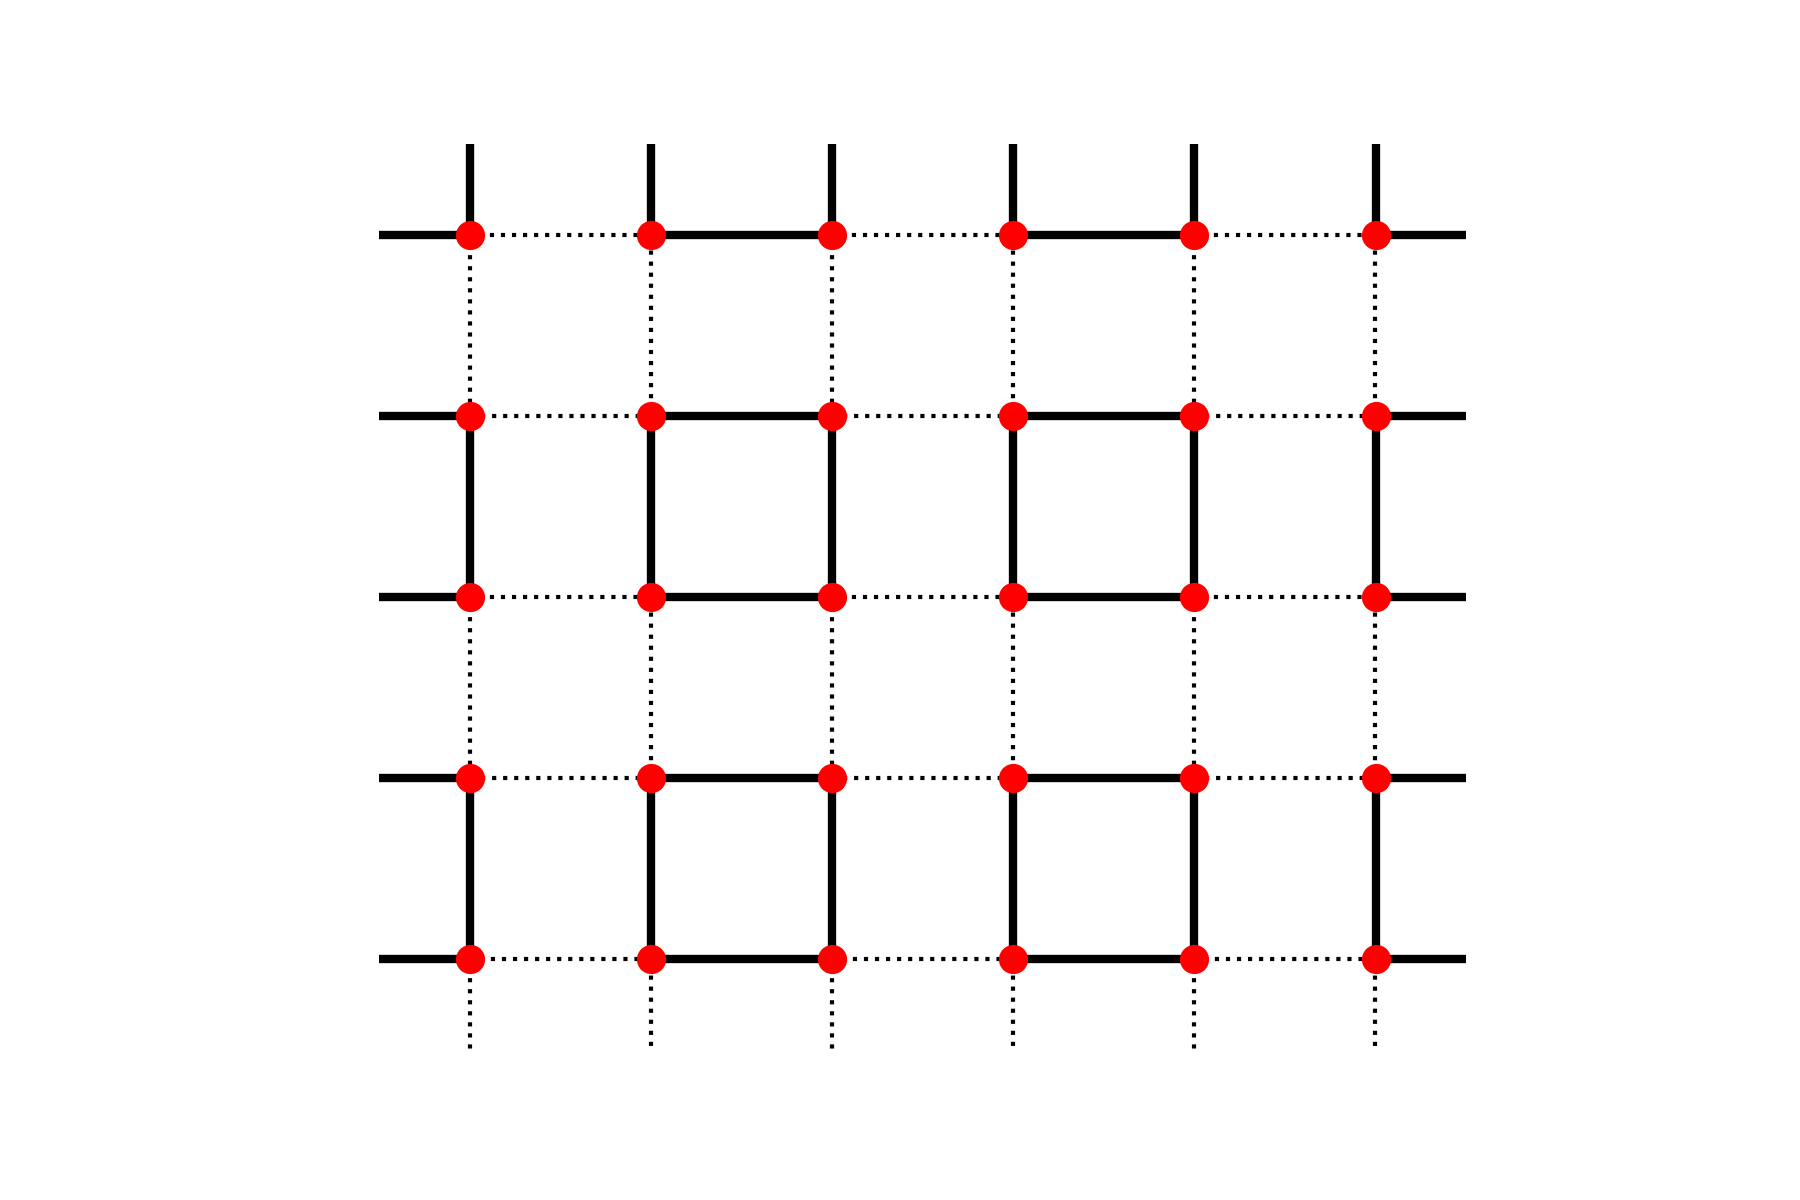
\includegraphics[scale=0.5]{Splitting_the_grid.png}
\centering 
\caption{Splitting grid in cells}
\label{fig:Splitting}
\end{figure}

For the lattice having \(N = N_1 + N_2\) knots   we will have
\[M = N / k \]
 cells (where \(k = 4\) in the  case under consideration).
 
 

Cells have to differ  by composition  and when composition  is the same -- by the arrangement of constituent atoms.

It is convenient to describe the values associated with a cell by a pair indexes \( i, \alpha \) where the first index 
indicates that the cell has \( i \) atoms of type 1 (and, correspondingly, \( k - i \) atoms of type 2) and the second index numbers all possible for the cell of specified content 
micro-configurations:
\[ \alpha = 1, 2, \dots \binom{k}{i} \]

In particular, let us denote  \( M_{i \alpha}\) the number of cells of type  \(  i, \alpha \)  and  \( U_{i \alpha} \) -- the internal energy of such cell (meaning the energy of links belonging to the cell).
Then we can express the total energy of all  links located inside  cells as

\begin{equation} \label{inside_energy}
E_{inside} = \sum_{i\alpha} U_{i \alpha} M_{i \alpha}
\end{equation} 

If we add to this quantity the energy $E_{outside}$ of all links located outside cells then the total energy of the system can be written as
\begin{equation} \label{energy2}
E = E_{inside} + E_{outside} 
\end{equation}

We cannot immediately present for $ E_{outside}$ a simple formula similar to (\ref{inside_energy}) but we can estimate it based on other arguments.

Cells were introduced above as purely formal entities; in particular, cells do not suppose existence of any Long  Range Order coherent with the cells selection.


It means that on the average we cannot distinct the links belonging to cells from the links between cells.

Therefore, comparing  $E_{inside}$ and $ E_{outside}$, we can conclude that these values can differ only as result of differences in the number of links  included, so   their ratio can be written as
\begin{equation} \label{ratio}
\frac{E_{outside}}{E_{inside}} = \frac{n_{outside}}{n_{inside}} 
\end{equation}
where $n_{outside}$ and ${n_{inside}}$ are counts of the links in the corresponding groups.

By adding one to both sides of (\ref{ratio}) we receive
\[
\frac{E}{E_{inside}} = \frac{z N / 2}{n_{inside}}
\]
where, naturally, $zN/2$ is the  total number of all links in the system.

Then the energy $E$ of entire grid can be written as


\begin{equation} \label{energy}
E = \beta\sum_{i\alpha} U_{i \alpha} M_{i \alpha}
\end{equation} 
where  
\[
\beta = \frac{z N / 2}{m M}
\]
and $m$ is the count of the links inside one cell.


The equation (\ref{energy}) is an immediate consequence of the basic assumption that introduced here cells have nothing in common with "clusters" or "associates" and have to be considered as purely formal entities.


It may be not evident at this moment but  the formula (\ref{energy}) -- the ability to use uniform expression for both parts of the energy, as defined in (\ref{energy2}) -- is responsible for radical simplification of the entire formalism. 


Continuing the   free energy construction we can now express the composition of alloy  through the introduced above  symbols:
\begin{equation} \label{N1}
    N_1 = \sum_{i\alpha} i M_{i \alpha}
\end{equation}
\begin{equation} \label{N2}
  \quad  \quad   \quad   N_2 = \sum_{i\alpha} (k-i) M_{i \alpha}
\end{equation}


The expression for the combinatorial factor \cite{Hill1956} is more complicated and will be constructed in a several steps. 


The starting point is the Bragg--Williams approximation \cite{Hill1956} that neglects all correlations and assumes that system allows perfect atom permutations:

\begin{equation} \label{bragg}
K_0 = \frac{N!}{N_1! N_2!}
\end{equation}

We will take this formula as the basic approximation.

The interatomic interactions  cause deviations in the atom distribution from the chaotic order and if we want to take in the account these deviations we should consider only macro-configurations that have this modified distribution.

 Mathematically this means that we switch from permutations of separate atoms to permutations of cells as whole: 


\begin{equation} \label{K1}
K_1 = \frac{M!}{\prod\limits_{i \alpha} ( M_{i \alpha})!}
\end{equation}

We would like to treat this expression as alternative   combinatorial  factor but for this purpose we  must be sure that it satisfies two conditions:

    - It achieves maximal value at the chaotic atom distribution;

    - It is correctly normalized at this condition providing the same value as  the equation (\ref{bragg}).


To be sure that chaotic distribution in the system is achieved we will consider the high temperature limit when the role of energy contribution (\ref{energy}) can be neglected. In addition, we should not forget the conditions (\ref{N1}) and (\ref{N2}) to make the result of maximization process compatible with (\ref{bragg}).


We will provide this calculation later in a more general form and for now we will base our consideration on the intuitively transparent result (that becomes completely evident if we remember that in chaotic approximation every knot of the lattice is populated independently of others and depends on the alloy composition only):
\[
M_{i\alpha}^\infty = M x_1^i x_2^{k-i}
\]
where the superscript $\infty$ indicates the high temperature limit and $x_j = N_j / N$ is the molar fraction of component $j$. We can now use this expression and equations (\ref{N1}) - (\ref{N2}) to calculate the value of $K_1^\infty$:
\[
\begin{split}
\ln{K_1^\infty} &= M \ln{M} - \sum_{i \alpha}M_{i\alpha}^\infty \ln{M_{i\alpha}^\infty}\\ &=  M \ln{M} - \sum_{i \alpha} M_{i\alpha}^\infty \left( \ln M + i \ln x_1 + (k-i) \ln x_2
\right)\\ &= - N_1 \ln x_1 - N_2 \ln x_2 = \ln K_0
\end{split}
\]

This formula is very important. Technically, it shows that $K_1$  is indeed acceptable expression ready to be used as  combinatorial  factor. More important, it confirms the main idea of TISR that in order to properly describe the configurational entropy one must consider all variations of local composition, avoiding the popular attempt to restrict formalism by an "average" or "most important" configurations.
   

After showing that $K_1$ is an acceptable combinatorial factor, the next step will be to show that we can immediately improve it.

Returning back to the fig.\ref{fig:Splitting} we can say that the combinatorial factor $K_1$ takes in the account the atom correlations associated with the links localized inside cells. The links outside of cells are completely neglected.

We can see also that these neglected links (dotted lines in the picture) form by itself a set of $2\times 2$ cells that is in any respect similar to the original set. Naturally, we want to include correlations associated with this second cell set into the combinatorial  factor.

Transition from the Bragg-Williams approximation $K_0$ to $K_1$ can be represented formally as applying some multiplicative correction factor to $K_0$:
\begin{equation} \label{config_1}
K_1 = K_0 * \left( \frac{K_1}{K_1^\infty} \right) =  K_0 * \left( \frac{K_1}{K_0} \right) 
\end{equation}

Since we have \textit{two} sets of cells we would like to accept  the following expression for the combinatorial factor: 

\begin{equation} \label{config_final}
K =K_0 * \left( \frac{K_1}{K_0} \right)^\gamma 
\end{equation}
where $\gamma=2$ for the simple square lattice.

In general case the value of $\gamma$ can be estimated similar to the way the $\beta$ value was evaluated: for the case depicted in the fig.\ref{fig:Splitting} one set of cells is responsible for $m M$ links belonging to this set; we need $\gamma$ sets to ensure all $z N/2$ links are taken into account:
\begin{equation} \label{gamma}
\gamma = (z N/2) / (m M)
\end{equation}

In the case under consideration $m = 4$, so we receive again that   $\gamma = 2$.


For the tetrahedron cell in the face-centered cubic  structure $\gamma=4$. 


We have now all necessary elements to construct the expression for the free energy:

\begin{equation} \label{free_energy}
\begin{split}
    F &= \beta\sum_{i\alpha} U_{i \alpha} M_{i \alpha} - \theta(1- \gamma) \ln K_0 - \theta \gamma \ln K_1\\ &+ \lambda_1 \left(N_1 - \sum_{i\alpha} i M_{i \alpha} 
    \right) + \lambda_2 \left(N_2 - \sum_{i\alpha} (k-i) M_{i \alpha} 
    \right)
\end{split}
\end{equation}
where $\theta $ is a temperature factor --  composition of absolute temperature and the Boltzmann constant $k_B$  \cite{Hill1956}; $\lambda_1$ and  $\lambda_2$ are the Lagrange multipliers  \cite{Arfken2013}.
Taking in the account that
\[
\ln K_1 = M \ln{M} - \sum_{i \alpha}M_{i\alpha} \ln{M_{i\alpha}}
\]
we can now get the basic equations of model:
\begin{equation} \label{basic_equation}
    \frac{\partial F}{\partial M_{i\alpha}} = \beta U_{i \alpha} + \theta \gamma \ln p_{i \alpha} - i \lambda_1 - (k-i) \lambda_2 = 0 
\end{equation}
where $ p_{i\alpha} =  M_{i\alpha} / M$.
Solution of these equations can be immediately written as
\begin{equation} \label{pia}
    p_{i\alpha} = \exp \left(- {\frac{\beta U_{i \alpha}}{\theta\gamma }}\right) b_1^i b_2^{k-i}
\end{equation}
where $b_j$ are defined through
\begin{equation}
    \lambda_j = \theta \gamma \ln b_j, \quad  j = 1, 2
\end{equation}

Taking in the account the explicit dependency of $K_0$ on $N_j$ (\ref{bragg}) we can now calculate the chemical potentials of components $\mu_j$ using the expression for the free energy (\ref{free_energy}):

\begin{equation} \label{chim_pot}
    \mu_j = \frac{\partial F}{\partial N_j} =  \theta (1 - \gamma) \ln x_j + \lambda_j = \theta \ln x_j + \theta \gamma \ln \frac{b_j}{x_j}
\end{equation}

We introduce now a few additional variables that will help to present solution to the above equations in a parametric form.
The specific form of the dependency of expression (\ref{pia}) on $b_i$ makes it convenient to introduce a new reduced notation $p_i$:
\begin{equation} \label{pi}
    p_i = \sum_\alpha p_{i \alpha} = W_i b_1^i b_2^{k-i}
\end{equation}
where
\begin{equation} \label{Wi}
    W_i = \sum_\alpha \exp \left(- {\frac{\beta U_{i \alpha}}{\theta\gamma }}\right)
\end{equation}
can be treated as the statistical sum \cite{Hill1956}
of the cell containing $i$ atoms of type 1 (and $k-i$ atoms of type 2). Renormalization factor $\beta / \gamma$ in this expression is responsible for the fact that every cell is part of endless grid rather than a separate object.

The new variables can be used to rewrite the equations (\ref{N1}) and (\ref{N2}) in a more compact form:


\begin{equation} \label{sum}
    \sum_i p_i = b_2^k \sum_i W_i c^i = 1 
\end{equation}
\begin{equation} \label{sumx1}
    \sum_i i p_i = b_2^k \sum_i i W_i c^i = k x_1 
\end{equation}
where the new notation $c$ 
\begin{equation} \label{c=}
    c := b_1 / b_2
\end{equation}
was introduced to be used as an independent variable for parametric representation both of composition and thermodynamic activities of components.


First, the equation (\ref{sum}) defines $b_2$ as a simple  function of $c$. Then the equation (\ref{c=}) defines $b_1$ as a function of $c$. This information can be directly substituted into expressions for $x_1$ and $\mu_j$ completing the calculation.

The necessary basis for the described calculation is the  knowledge of $W_i$ that will be treated in the following text as the model parameters. As is evident from the definition (\ref{Wi}), when $\theta \to \infty$ we will get the limiting value $$W_i^\infty = \binom{k}{i}$$
Inserting this expression into the previous three equations we immediately receive the limiting values
$$ b_j^\infty = x_j; \quad p_{i \alpha}^\infty = x_1^i x_2^{k-i}$$
This result is independent of the value of $\gamma$ in (\ref{free_energy}) and if we assume $\gamma = 1$ (it is the condition at which the minimum of $F$  is precisely equivalent to the maximum of combinatorial factor $K_1$) we can see that $p_{i \alpha}^\infty$ has just the value already announced during the discussion the high temperature behavior of the  combinatorial  factor (\ref{K1}).

At finite temperatures (as mentioned in the Introduction) the  $W_i$ parameters can be easily deduced from the experimental data if the chemical potentials of all components are known.

Indeed, if for some composition $x_j$ we know the chemical potentials of components $\mu_j$ then from the equation (\ref{chim_pot}) we can found both $b_j$. By substituting these values into  (\ref{sum}) we receive equation where the only unknown entities are $W_i$. Since this equation is linear in respect to unknowns, we can use linear regression analysis \cite{Regression2016} to estimate $W_i$.

Applying the standard thermodynamic formulas \cite{Prigogine1954} to the expression for the free energy (\ref{free_energy}) and remembering definition (\ref{Wi}) of $W_i$  we can calculate the integral enthalpy of the system:

\begin{equation} \label{H}
\begin{split}
    H &= - \theta^2 \frac{\partial( F/\theta)}{\partial \theta} - \theta^2 \sum_{i \alpha}\frac{\partial (F/\theta)}{\partial M_{i\alpha}} \frac {\partial M_{i\alpha}} {\partial \theta} - \theta^2 \sum_j\frac{\partial (F/\theta)}{\partial \lambda_j} \frac {\partial \lambda_j} {\partial \theta} \\
    &= - \theta^2 \beta\sum_{i \alpha} \frac{\partial (U_{i \alpha}/\theta)}{\partial \theta} M_{i \alpha}
    = \gamma\theta^2  M \sum_i \frac{\partial W_i}{\partial \theta} b_1^i b_2^{k-i}\\
    &= \gamma\theta^2  M \frac{\sum\limits_i c^i \partial W_i/\partial \theta}{\sum\limits_i c^i W_i }
\end{split}    
\end{equation}

Assuming that $W_i$ are already determined from the thermodynamic activities of components we can use the last equation to estimate $\partial W_i / \partial \theta$ from the data on integral  enthalpy -- again using linear regression analysis.

Calculation of partial  enthalpy of components is a little bit more involving. According to (\ref{H}) $H$ is an explicit function of $c$ and we can revert the formulas (\ref{sum}) --  (\ref{sumx1}) to consider c as a function of $x_1$. Using these formulas we can calculate the following derivative:


\begin{equation} \label{dc2dx1}
    \frac{\partial c}{\partial x_1} = 2 k \frac{
    \left(\sum\limits_i W_i c^i\right)^2}{\sum\limits_{i, l} \left(i-l \right)^2 W_i W_l c^{i+l-1}}
\end{equation}

 We can now express the partial  enthalpy of components (denoting   $h = H / N$) as:

\begin{equation}
\begin{split}
    \bar h_1  =  \frac{\partial H}{\partial N_1} = h + x_2\frac{\partial h}{\partial c} \frac{\partial c}{\partial x_1}\\
    \bar h_2  =  \frac{\partial H}{\partial N_2} = h - x_1\frac{\partial h}{\partial c} \frac{\partial c}{\partial x_1}
\end{split}
\end{equation}
where the derivative $\partial h / \partial c$ can be directly calculated  from the equation (\ref{H}).


\section{Critical Point}

The just introduced $\gamma$ and $\beta$ parameters turned out to have the same value in the previous section. It is shown in \cite{TISR_p2} that  the provided choice ensures the accuracy of theory close to the accuracy of Quasichemical Theory or better.

While the choice of $\beta$ is clearly and in details discussed at the beginning of the previous section, the selection of $\gamma$ may raise  some questions.

In fact, the final value of $\gamma$ in (\ref{gamma}) is based solely on the  assumption that distribution of links within one ensemble of cells  is completely independent from the existence  of other similar ensembles.


In classical literature devoted to QT this type of  assumption was named "non-interference  hypothesis"  \cite{GUGGENHEIM1952}.

This hypothesis looks quite plausible at high temperatures  but hardly could be justified in the critical region where the correlation length aims to infinity.

It can be expected  that in the close proximity to the critical point the knowledge of correlations associated with one cell ensemble provides at least partial information about correlations associated with   other ensembles. 

Effectively, it may mean that near the critical point  the effective value of $\gamma$  could be less than it is suggested by the  "non-interference  hypothesis" and defined by expression (\ref{gamma}).


Unfortunately, there are no simple approaches to assess how the  effect under discussion can      affect the value of           $\gamma$.


It turns out  however \cite{KREMER1985, tisr1988} that it is quite possible to impose on  $\gamma$ an additional condition which will ensure  the reproduction of  the correct critical temperature  of immiscibility and at the same time  significantly improve the calculated values of the  most important thermodynamic quantities.


This $\gamma$ adjustment should be done best within the framework of the Ising model  -- i.e. the environment that provides comprehensive list of data related to the critical behavior \cite{Domb1974} and therefore a good reference base for comparison.
	

It is why we want now to derive a few simple formulas that will be handy when working with the immiscibility phenomenon.

We continue to use  the standard assumptions of the Ising model \cite{Domb1974}, which means, in particular, that the curve representing the dependency of  free energy on the composition is symmetrical with respect to  the concentration $x = 1/2$.


It means also that the immiscibility curve (binodal \cite{Hillert2008}) can be described as not trivial $(x \neq 1/2$) solution of the  equation
\begin{equation} \label{immiscibility}
\frac{\partial f}{\partial x_1}  \equiv \mu_1(x_1) - \mu_2(x_1) = 0
\end{equation}

Using the equation (\ref{chim_pot}) for the chemical potential and definition (\ref{c=}) of $c$ we can interpret (\ref{immiscibility}) as equation on $c$:

\begin{equation} \label{immiscibility2}
\frac{\partial f}{\partial x_1} = \theta (1 - \gamma) \ln{\frac{x_1}{x_2}} + \theta \gamma \ln{c} = 0
\end{equation}
or

\begin{equation} \label{unmix_curv}
% \gamma \log c = (\gamma - 1) \log \frac{x_1}{x_2}
\frac {x_1(c)}{x_2(c)} = c ^{\frac{\gamma}{\gamma - 1}}
\end{equation}

The solution of this equation with respect to  $c$  together with the equation (\ref{sumx1}) define binodal in a parametric form.


Critical point corresponds to $x_1 = 0.5$ when $c = 1$. Unfortunately, at this conditions the equations (\ref{unmix_curv}) turns into identity. Resolving this uncertainty we coming to the final expression for the critical point:

 \begin{equation} \label{crit_point}
 \frac{\gamma}{\gamma - 1} = \lim_{c \to 1} \frac{x_1(c) - x_2(c)}{(c - 1) x_2(c)}
\end{equation}


To derive the equation for spinodal \cite{Hillert2008} we would like to consider $c$ and the entire right side of (\ref{immiscibility2}) as function of $x_1$. As result, spinodal is defined by equation

 \begin{equation} \label{spinodal}
 \frac{\partial^2 f}{\partial x_1^2} \equiv \theta (1 -\gamma)  (\frac{1}{x_1} + \frac{1}{1 - x_1})  + \theta \gamma \frac{1}{c} \frac{dc}{dx_1} = 0
\end{equation}

Using (\ref{dc2dx1}) we can bring this equation to the final form:
\begin{equation} \label{spinodal2}
 (1 -\gamma) k   \sum\limits_{i, l} \left(i-l \right)^2 W_i W_l c^{i+l} + 2  \gamma \sum\limits_i i   W_i c^i \sum\limits_l  (k-l) W_l c^l  = 0
\end{equation}


All the above manipulations are purely formal in nature and do not guarantee the   existence of immiscibility at all. 
From the  equation (\ref{crit_point})  it is evident that the value $\gamma = 1$ may be singular, but the problems can be found even when 
$\gamma > 1$.  


As an example, in the next part of this publication \cite{TISR_p2} the formalism with $k=2$ will be used to derive the equations of the Quasichemical Theory. It can be shown that in this case the equation  (\ref{crit_point}) has solution only when $\gamma > 2$.

In the part four of this publication \cite{TISR_p4} the suggested  choice of $\gamma$ will be discussed in details. It will be shown that 
the  modified combinatorial factor not only reproduces the correct critical temperatures for the Ising lattices but simultaneously  increases significantly the accuracy of thermodynamic calculations near the critical point.  

\section{Examples of Application}

This section includes several examples where Redlich-Kister based approximations \cite{Redlich1949} for thermodynamic functions reported by different authors are reinterpreted using TISR. Selection of sources was  random without any attempt to bring up  "good" cases only. 

In  all figures below the results of Redlich-Kister approximations are shown as solid lines. TISR calculations were performed in the tetrahedron approximation and results are presented by the dotted lines. The summary of results is available  in the table below (where $\theta * {\partial W_i}/{\partial \theta}$ is abbreviated as $dW_i$ for brevity):


\begin{table}[ht]
  \begin{center}
    \caption{TISR parameters adjusted to the available Redlich-Kister polynomials.}
    \label{tab:table1}
    \begin{tabular}{|c|c|SS|SS|SS|} % <-- Changed to S here.
	 \hline
      System &{Figure} & ${W_1}$ & ${dW_1}$ & ${W_2}$ & ${dW_2}$ & ${W_3}$ & ${dW_3}$\\
      \hline
Ag-In & fig.\ref{fig:Ag-In} & 5.722 & -0.271 & 10.747 & -4.883 & 11.364 & -6.433\\ \hline
Ag-Sb & fig.\ref{fig:Ag-Sb} & 4.979 & 0.959 & 6.372 & 2.428 & 8.739 & -4.637\\ \hline
In-Sb & fig.\ref{fig:In-Sb} & 6.171 & -3.78 & 10.4 & -7.822 & 6.171 & -3.781\\ \hline
Al-Ga & fig.\ref{fig:Al-Ga} & 4.133 & 0.219 & 6.279 & 0.448 & 4.023 & 0.347\\ \hline 
Al-Ni & fig.\ref{fig:Al-Ni} & 24.84 & -61.332 & 93.534 & -322.812 & 22.291 & -53.686\\ \hline
Al-Si & fig.\ref{fig:Al-Si} & 5.474 & -1.291 & 8.717 & -2.701 & 4.458 & -0.519\\ \hline
Al-Zn & fig.\ref{fig:Al-Zn} & 3.305 & 0.964 & 4.606 & 1.946 & 3.305 & 0.964\\ \hline
Ca-Ni & fig.\ref{fig:Ca-Ni} & 8.675 & -8.07 & 5.213 & -3.981 & 4.362 & -2.086\\ \hline
Cu-Si & fig.\ref{fig:Cu-Si2} & 6.432 & -2.626 & 9.002 & -1.898 & 13.077 & -20.173\\ \hline
Cu-Si & fig.\ref{fig:Cu-Si} & 5.511 & -1.724 & 8.52 & -2.49 & 7.394 & -13.796\\ \hline
La-Zr & fig.\ref{fig:La-Zr} & 2.136 & 1.692 & 2.673 & 3.423 & 2.626 & 1.405\\ \hline
    \end{tabular}
  \end{center}
\end{table}


\section{Conclusions}
The main idea of TISR is presentation of Short Range Order through the properties and relative amounts of small groups of atoms conventionally selected in the alloy. This approach allows to consider the wide range of systems -- from ones close to ideality to alloys with very high energetical intensity and structural inhomogeneity.

It has to be stressed out that the named groups of atoms are purely conventional and in this respect have nothing in common with hypothetical clusters or associates.

The most critical point of theory is the expression for combinatorial factor that ensures high precision in the limiting case of Ising model and, consequently, a good basis for usage in more complicated cases where we may not have precise results to be used as reference to estimate precision level. 


Exceptional advantage of suggested formalism is the fact that the introduced  combinatorial factor leads to a set of equations that can be explicitly solved in a parametric form.

The developed formalism starts by accepting  the basic rules of the Ising model but ultimately comes to  the result where all thermodynamic properties are expressed through the Statistical Sums $W_i$ of cells (\ref{Wi}) -- providing this way a huge economy in the number of empirical coefficients.

Such presentation opens also a straightforward path to the numerous generalizations of the physical model from the assumed Ising-like type of interatomic interaction to an arbitrary complicated picture that takes in the account  diverse non-Ising effects.

Since all details of interatomic interaction are hidden inside of  $W_i$ units, such generalization can be done without providing explicit assumptions about details of interaction -- feature that can have both positive and negative consequences.

As illustrative example, TISR was applied to multiple two-component systems described by different authors using Redlich-Kister approximation. Theory was taken in tetrahedron approximation and in most cases  reveals very high level of  accuracy in reproduction the thermodynamic data.

The main exclusion is the system Cu-Si in the fig.\ref{fig:Cu-Si2} where strange irregularities on the activity graph are thanks to the high level of Redlich-Kister polynomial used in \cite{Cu-Si2_Data}. The same system in the fig.\ref{fig:Cu-Si} was described in
 \cite{Al-Si_Data} by polynomial of lower degree and behaves much more regular.

\section{Related Publications}

The accent in this article is made on the description of \textit{liquid} alloys to emphasize  the unique role of  Short Range Order in this case, but in fact nothing in the developed approach prevents us from using it to describe the coexistence of Short and Long Range orders in \textit{solid} mixtures. 

Not identical, but technically close to this is the case of liquid alloys which, of course,  do not exhibit  Long Range Order in the classical sense but nevertheless manifest locally a two-lattice-like Short Range Order. If  alloy is known to have multi-lattice structure in solid phase it would be difficult to expect purely substitution-like Short Range Order in the liquid state.

Multi-lattice generalization is only one direction where TISR can be applied.

The advantage of TISR is that it is able to consider, within the framework of general formalism, a whole list of model theories traditionally considered independent or even inconsistent.

In this respect, the current publication has to be considered as introduction to the following list of related issues:

\begin{center}
 \begin{tabular}{p{60mm} p{90mm}} 
Article & Description \\ 
 \hline
 \hline
&\\
\href{https://osf.io/4hzf9/} {Part 2. Quasichemical Theory} &  Quasichemical Theory, presented as the partial case of  TISR,   is   critically compared with the Modified Quasichemical Model. \\
 & \\
\href{https://osf.io/7x2e4/}{Part 3. ASM Reconstructed} &Good known internal problems of Association Solution Model are completely explained and then resolved by presenting the revised form of ASM as the partial case of TISR.\\
& \\
\href{https://osf.io/zmwcv/}{Part 4. Combinatorial Factor}
& Improved combinatorial factor allows to reproduce the correct critical temperatures of alloys and simultaneously  significantly increases the precision of calculated thermodynamic quantities.\\
& \\
Theory generalizations&Formalism of TISR is extended on multicomponent mixtures and systems with Long Range Order.\\
&\\
Cluster Site Approximation & "Cluster Site Approximation" is presented as the partial case of TISR. Formalism of theory is significantly simplified.\\
&\\
Surrounded atom model & Combinatorial factor postulated by "Surrounded atom model" contains crude error that is automatically fixed  when model is reconstructed as the partial case of TISR. \\
&\\
Computational details& Computational algorithms of TISR are presented and visualized  using jupyter notebooks.
\end{tabular}
\end{center}





\bibliographystyle{unsrtnat}
\bibliography{D:/Thermo_Data/MQM/Article/references}

\begin{figure}[h]
\centering
\begin{subfigure}{.5\textwidth}
  \centering
  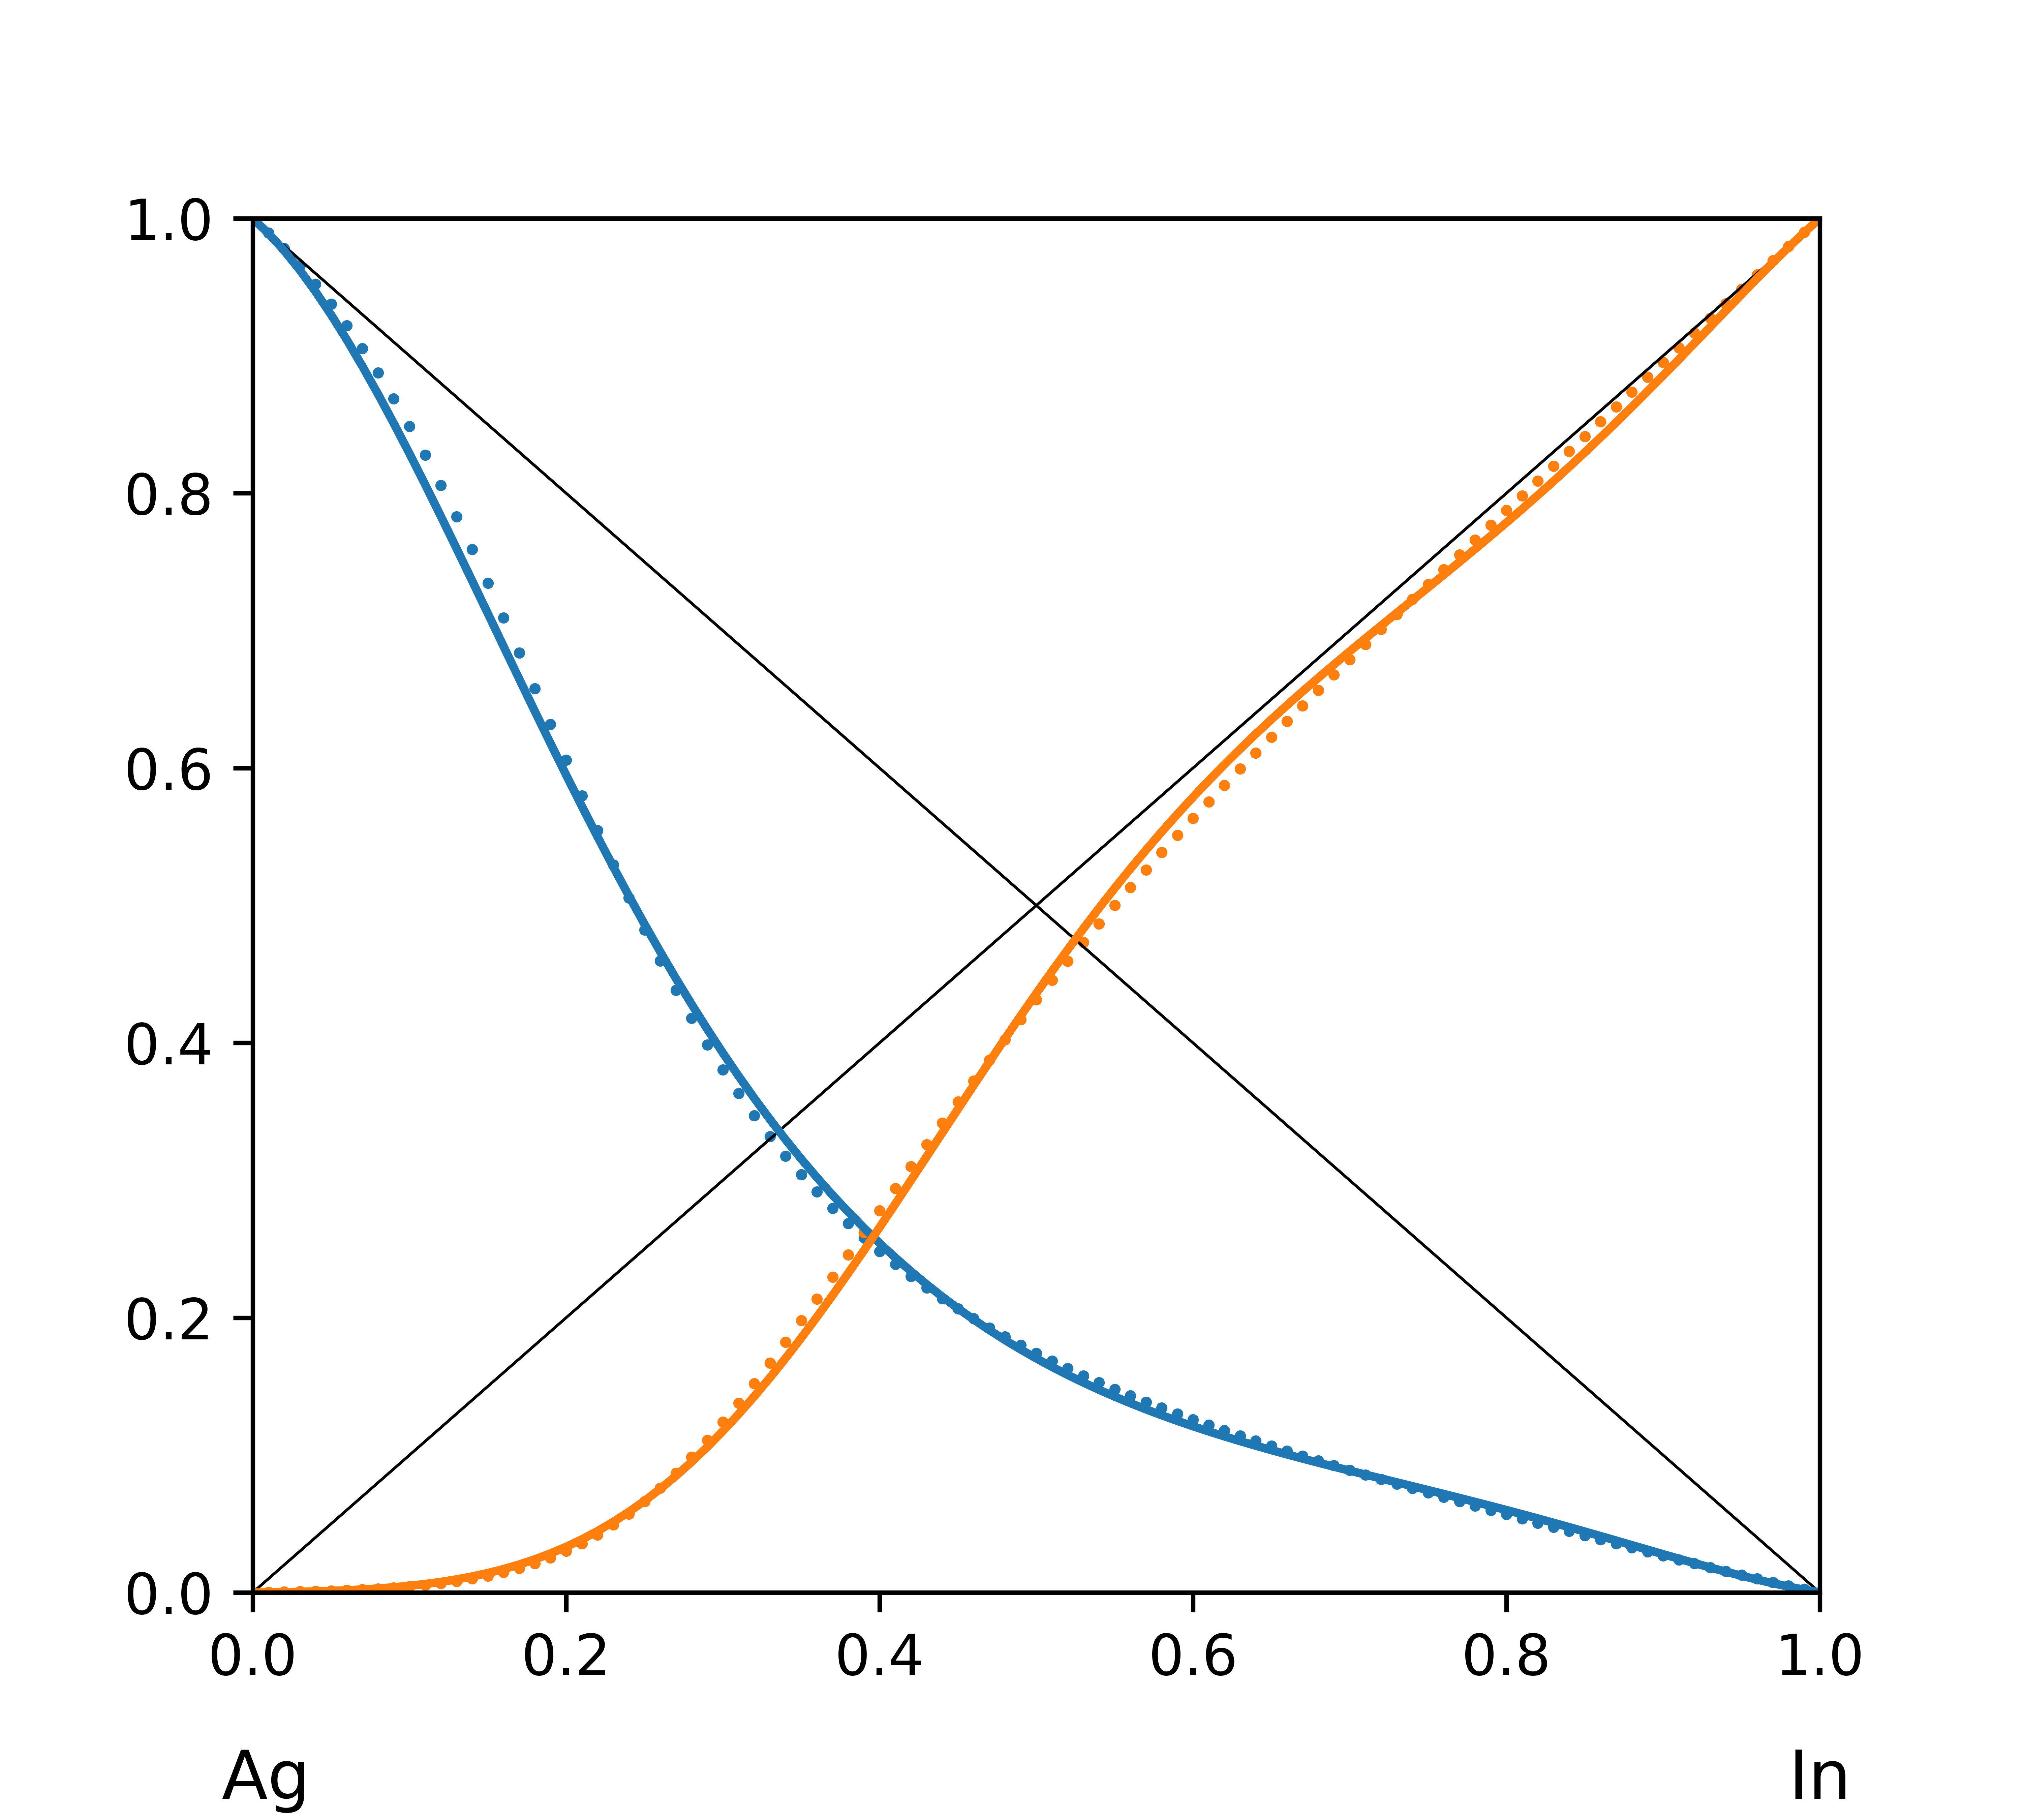
\includegraphics[width=1\linewidth]{Ag-In_Activity}
  \caption{Component Activities}
  \label{fig:Ag-In1}
\end{subfigure}%
\begin{subfigure}{.5\textwidth}
  \centering
  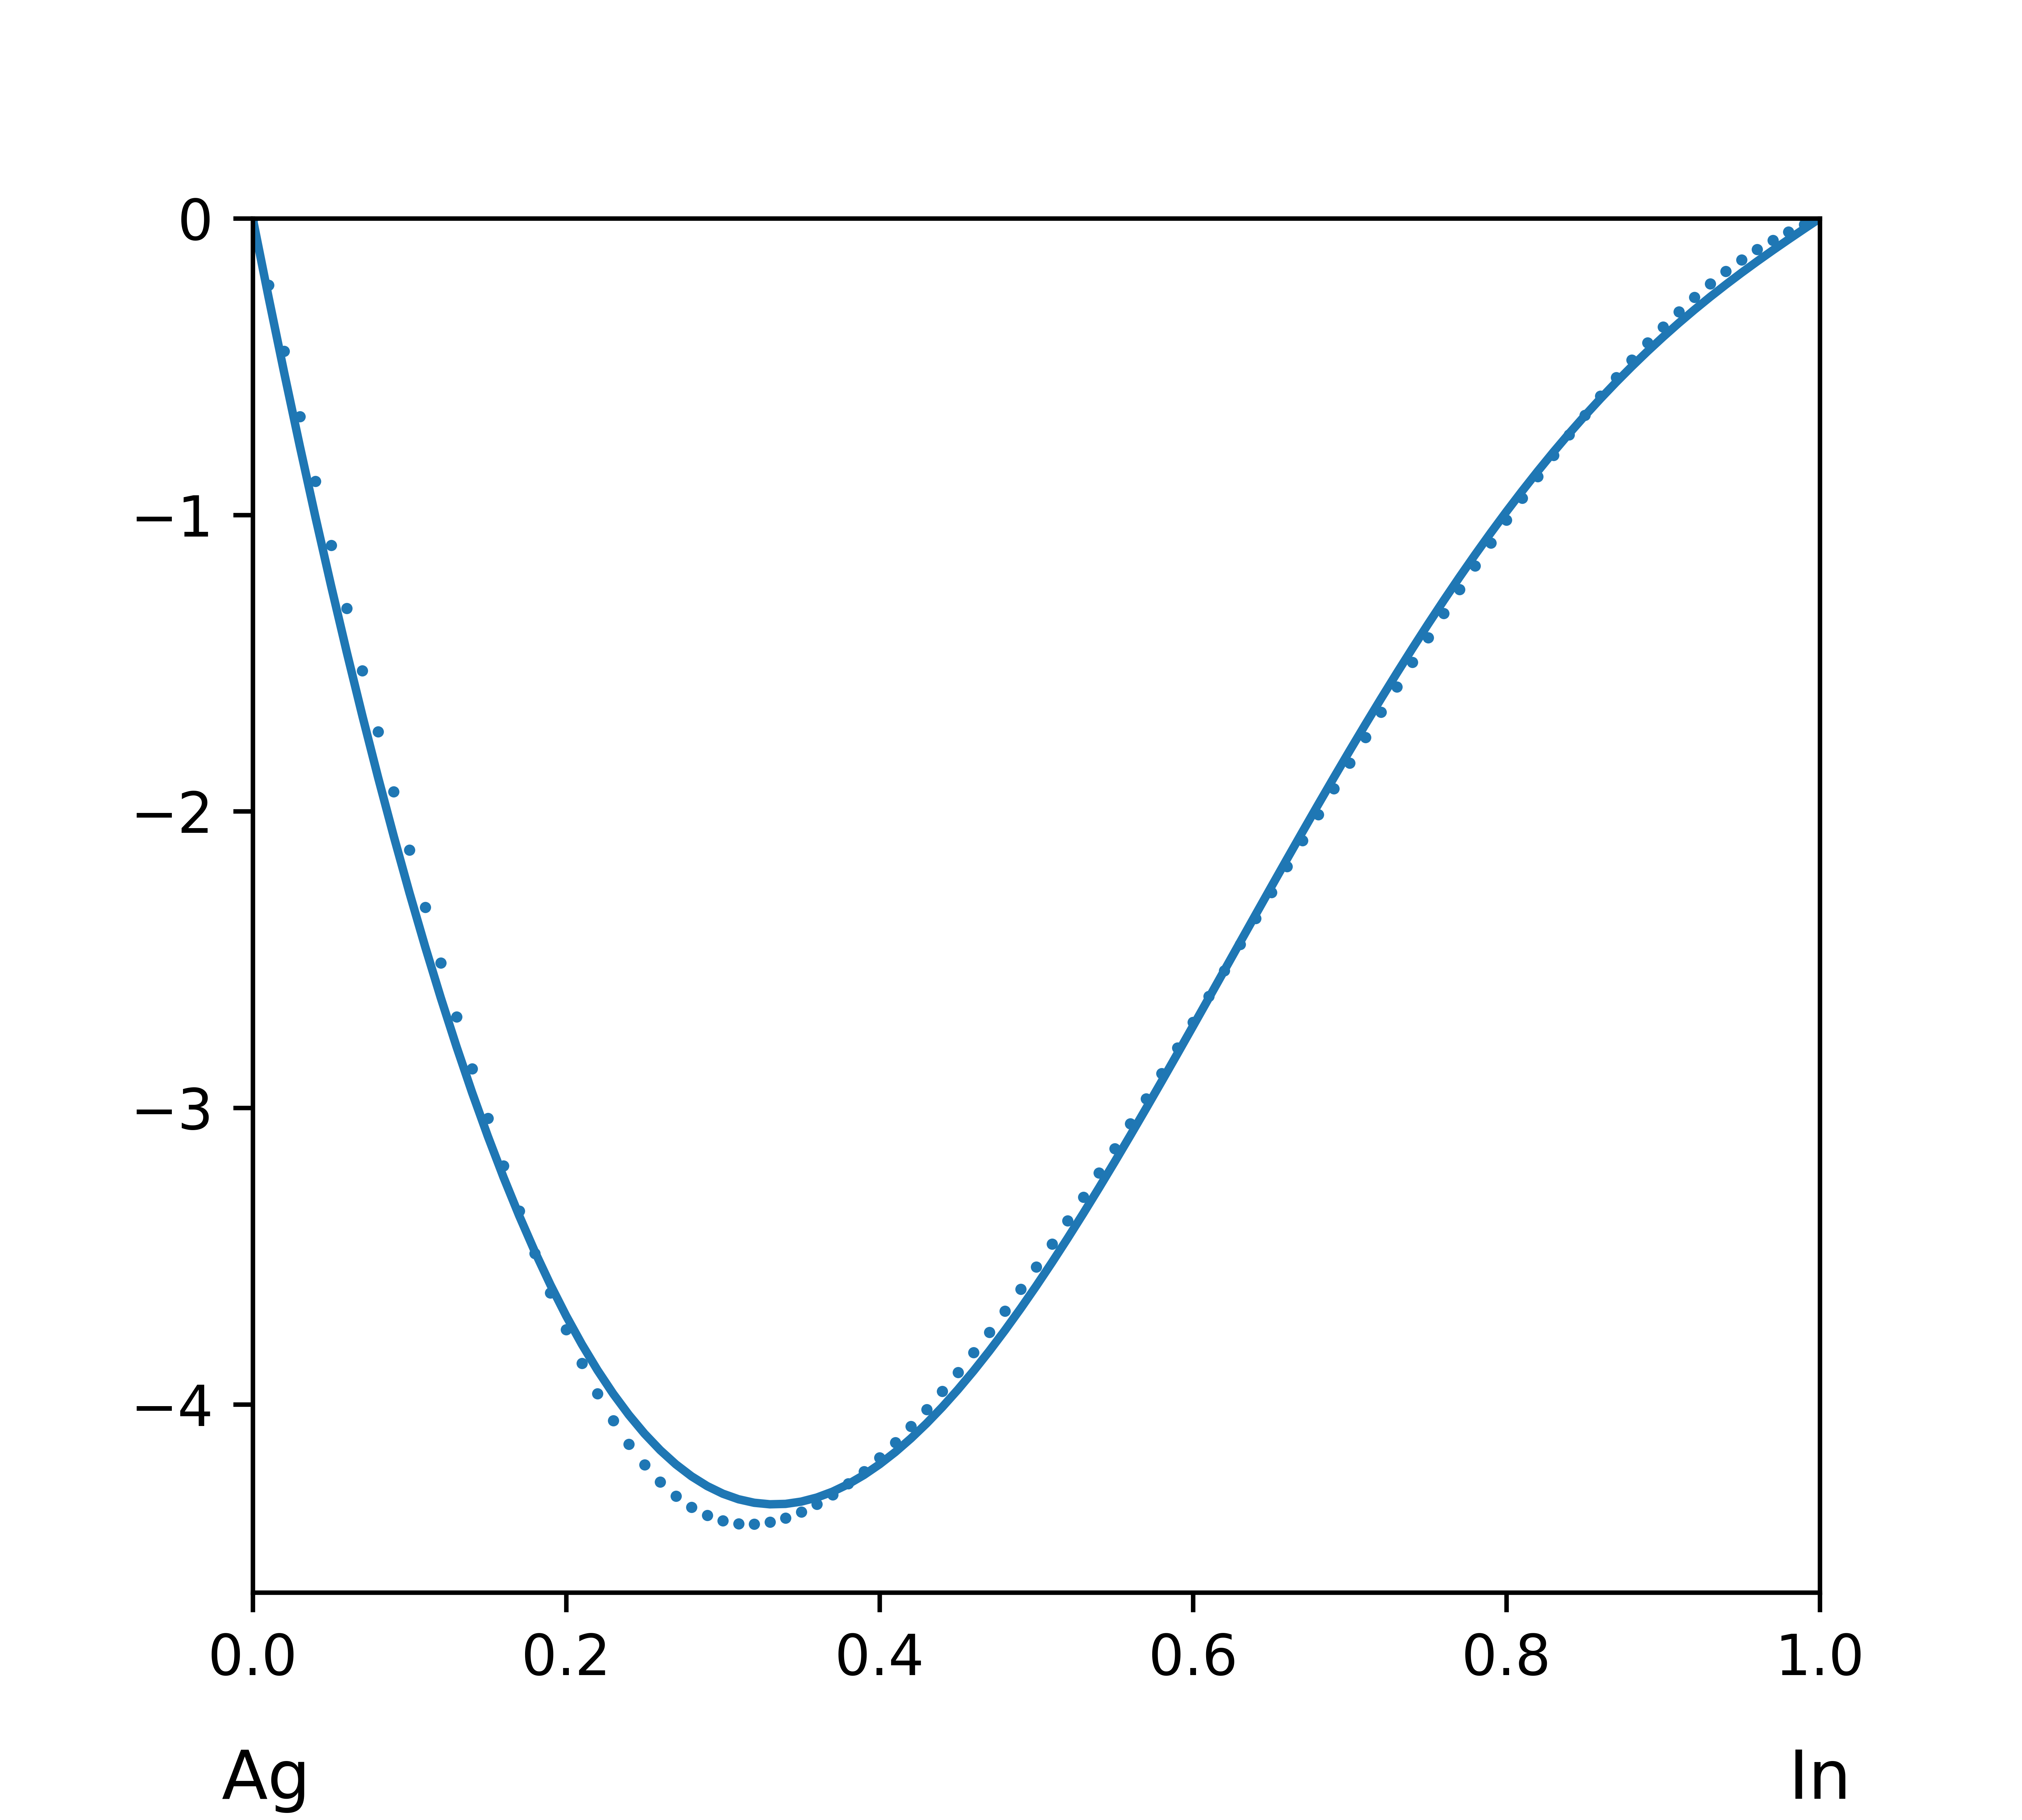
\includegraphics[width=1\linewidth]{Ag-In_Enthalpy}
  \caption{Enthalpy of Mixing (kJ/mol)}
  \label{fig:Ag-In2}
\end{subfigure}
\caption{System Ag-In (T = 1200 K): solid lines -- \cite{Ag-In_Data}; dotted lines - TISR}
\label{fig:Ag-In}
\end{figure}

\begin{figure}
\centering
\begin{subfigure}{.5\textwidth}
  \centering
  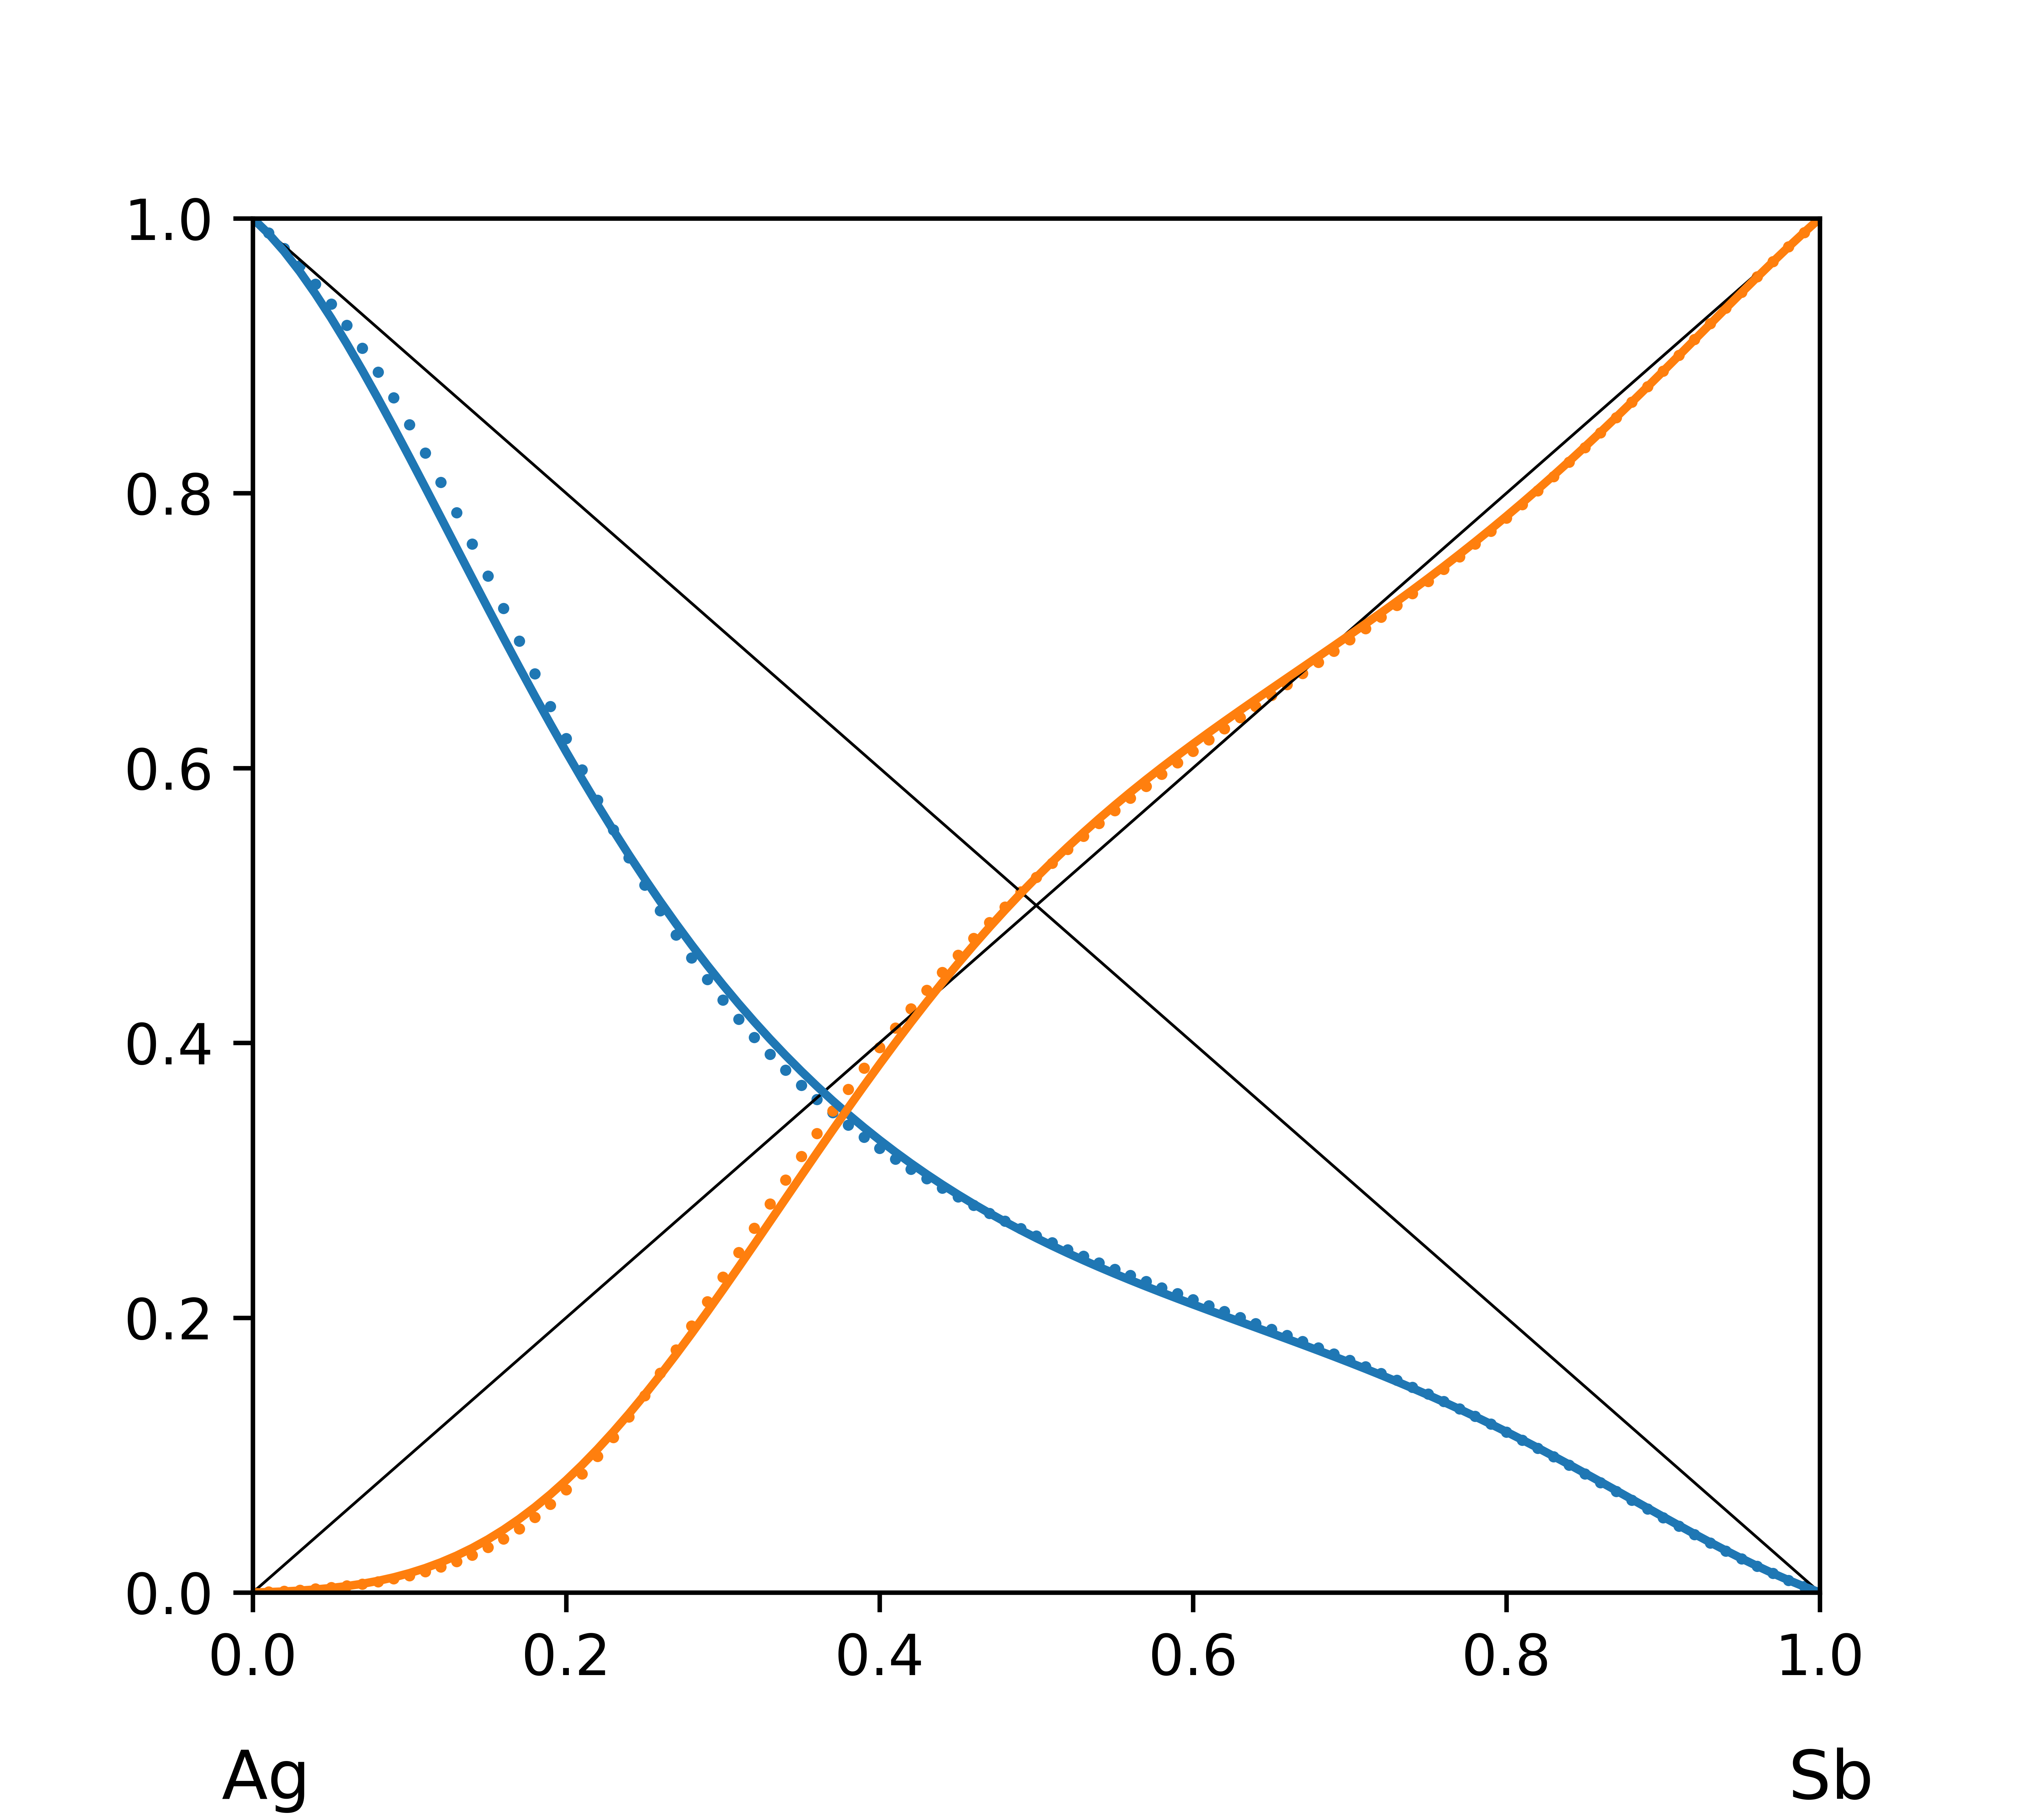
\includegraphics[width=1\linewidth]{Ag-Sb_Activity}
  \caption{Component Activities}
  \label{fig:sub1}
\end{subfigure}%
\begin{subfigure}{.5\textwidth}
  \centering
  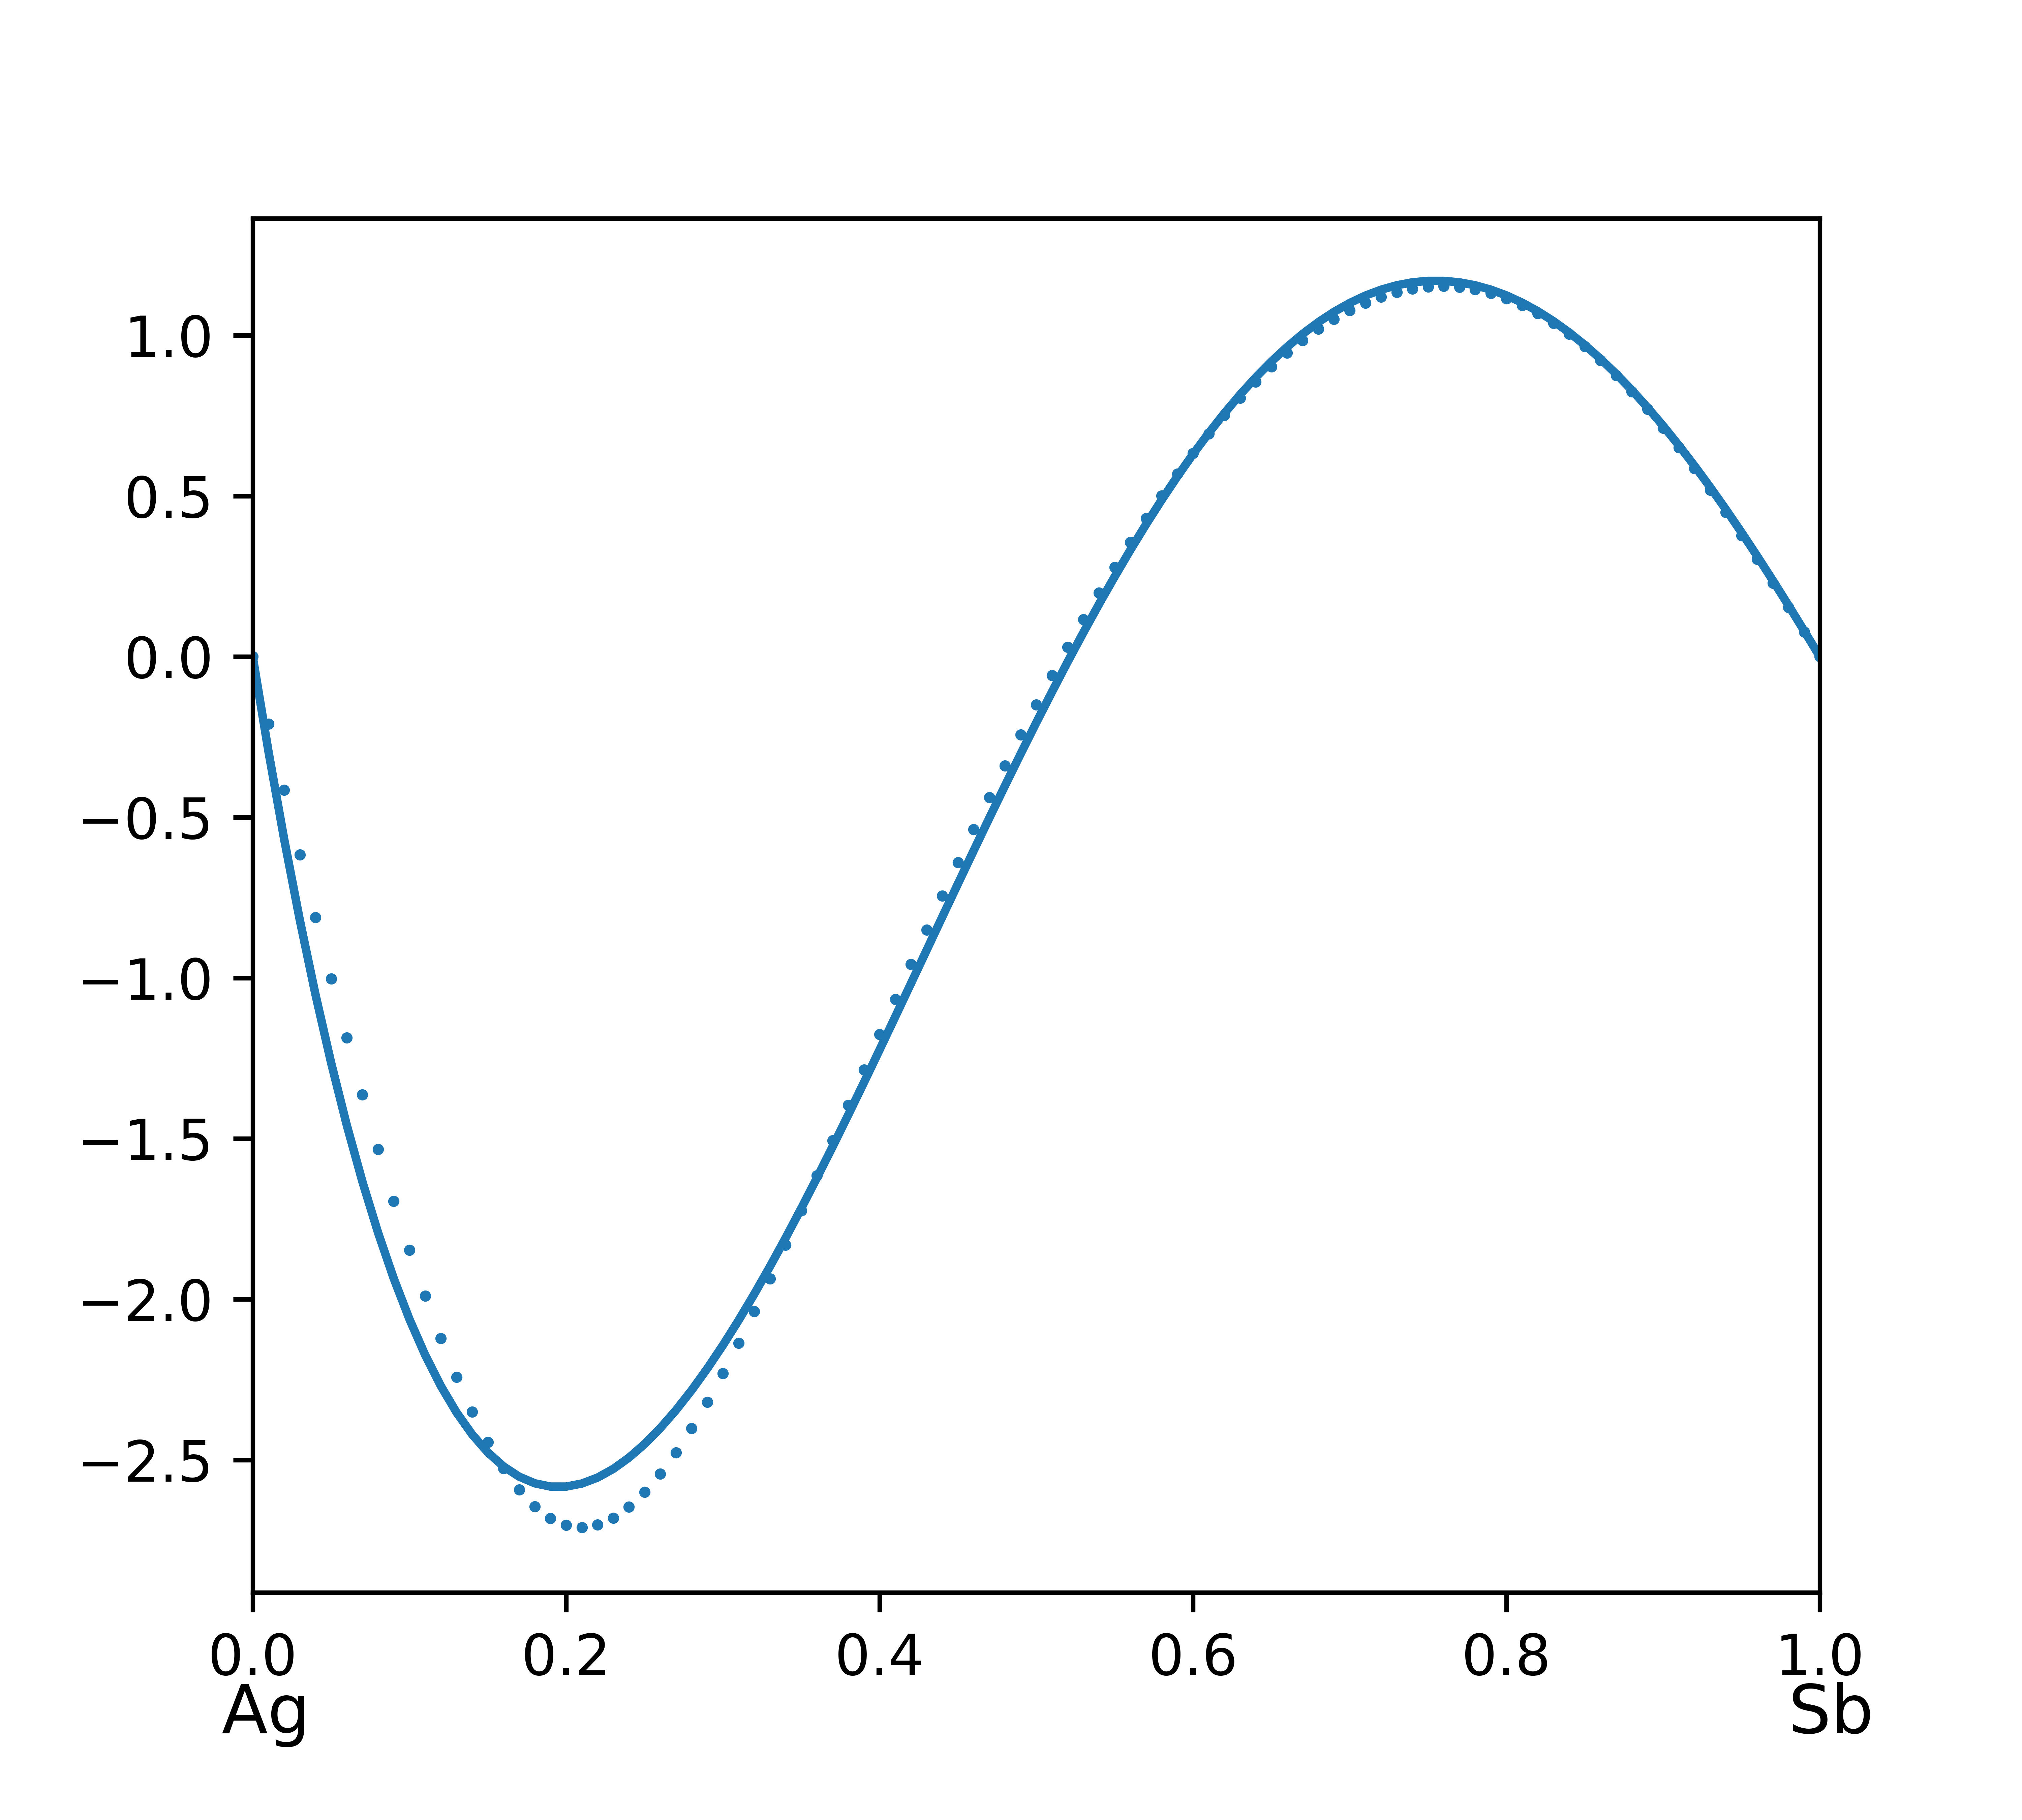
\includegraphics[width=1\linewidth]{Ag-Sb_Enthalpy}
  \caption{Enthalpy of Mixing (kJ/mol)}
  \label{fig:sub2}
\end{subfigure}
\caption{System Ag-Sb (T = 1200 K): solid lines -- \cite{Ag-In_Data}; dotted lines - TISR}
\label{fig:Ag-Sb}
\end{figure}


\begin{figure}[h]
\centering
\begin{subfigure}{.5\textwidth}
  \centering
  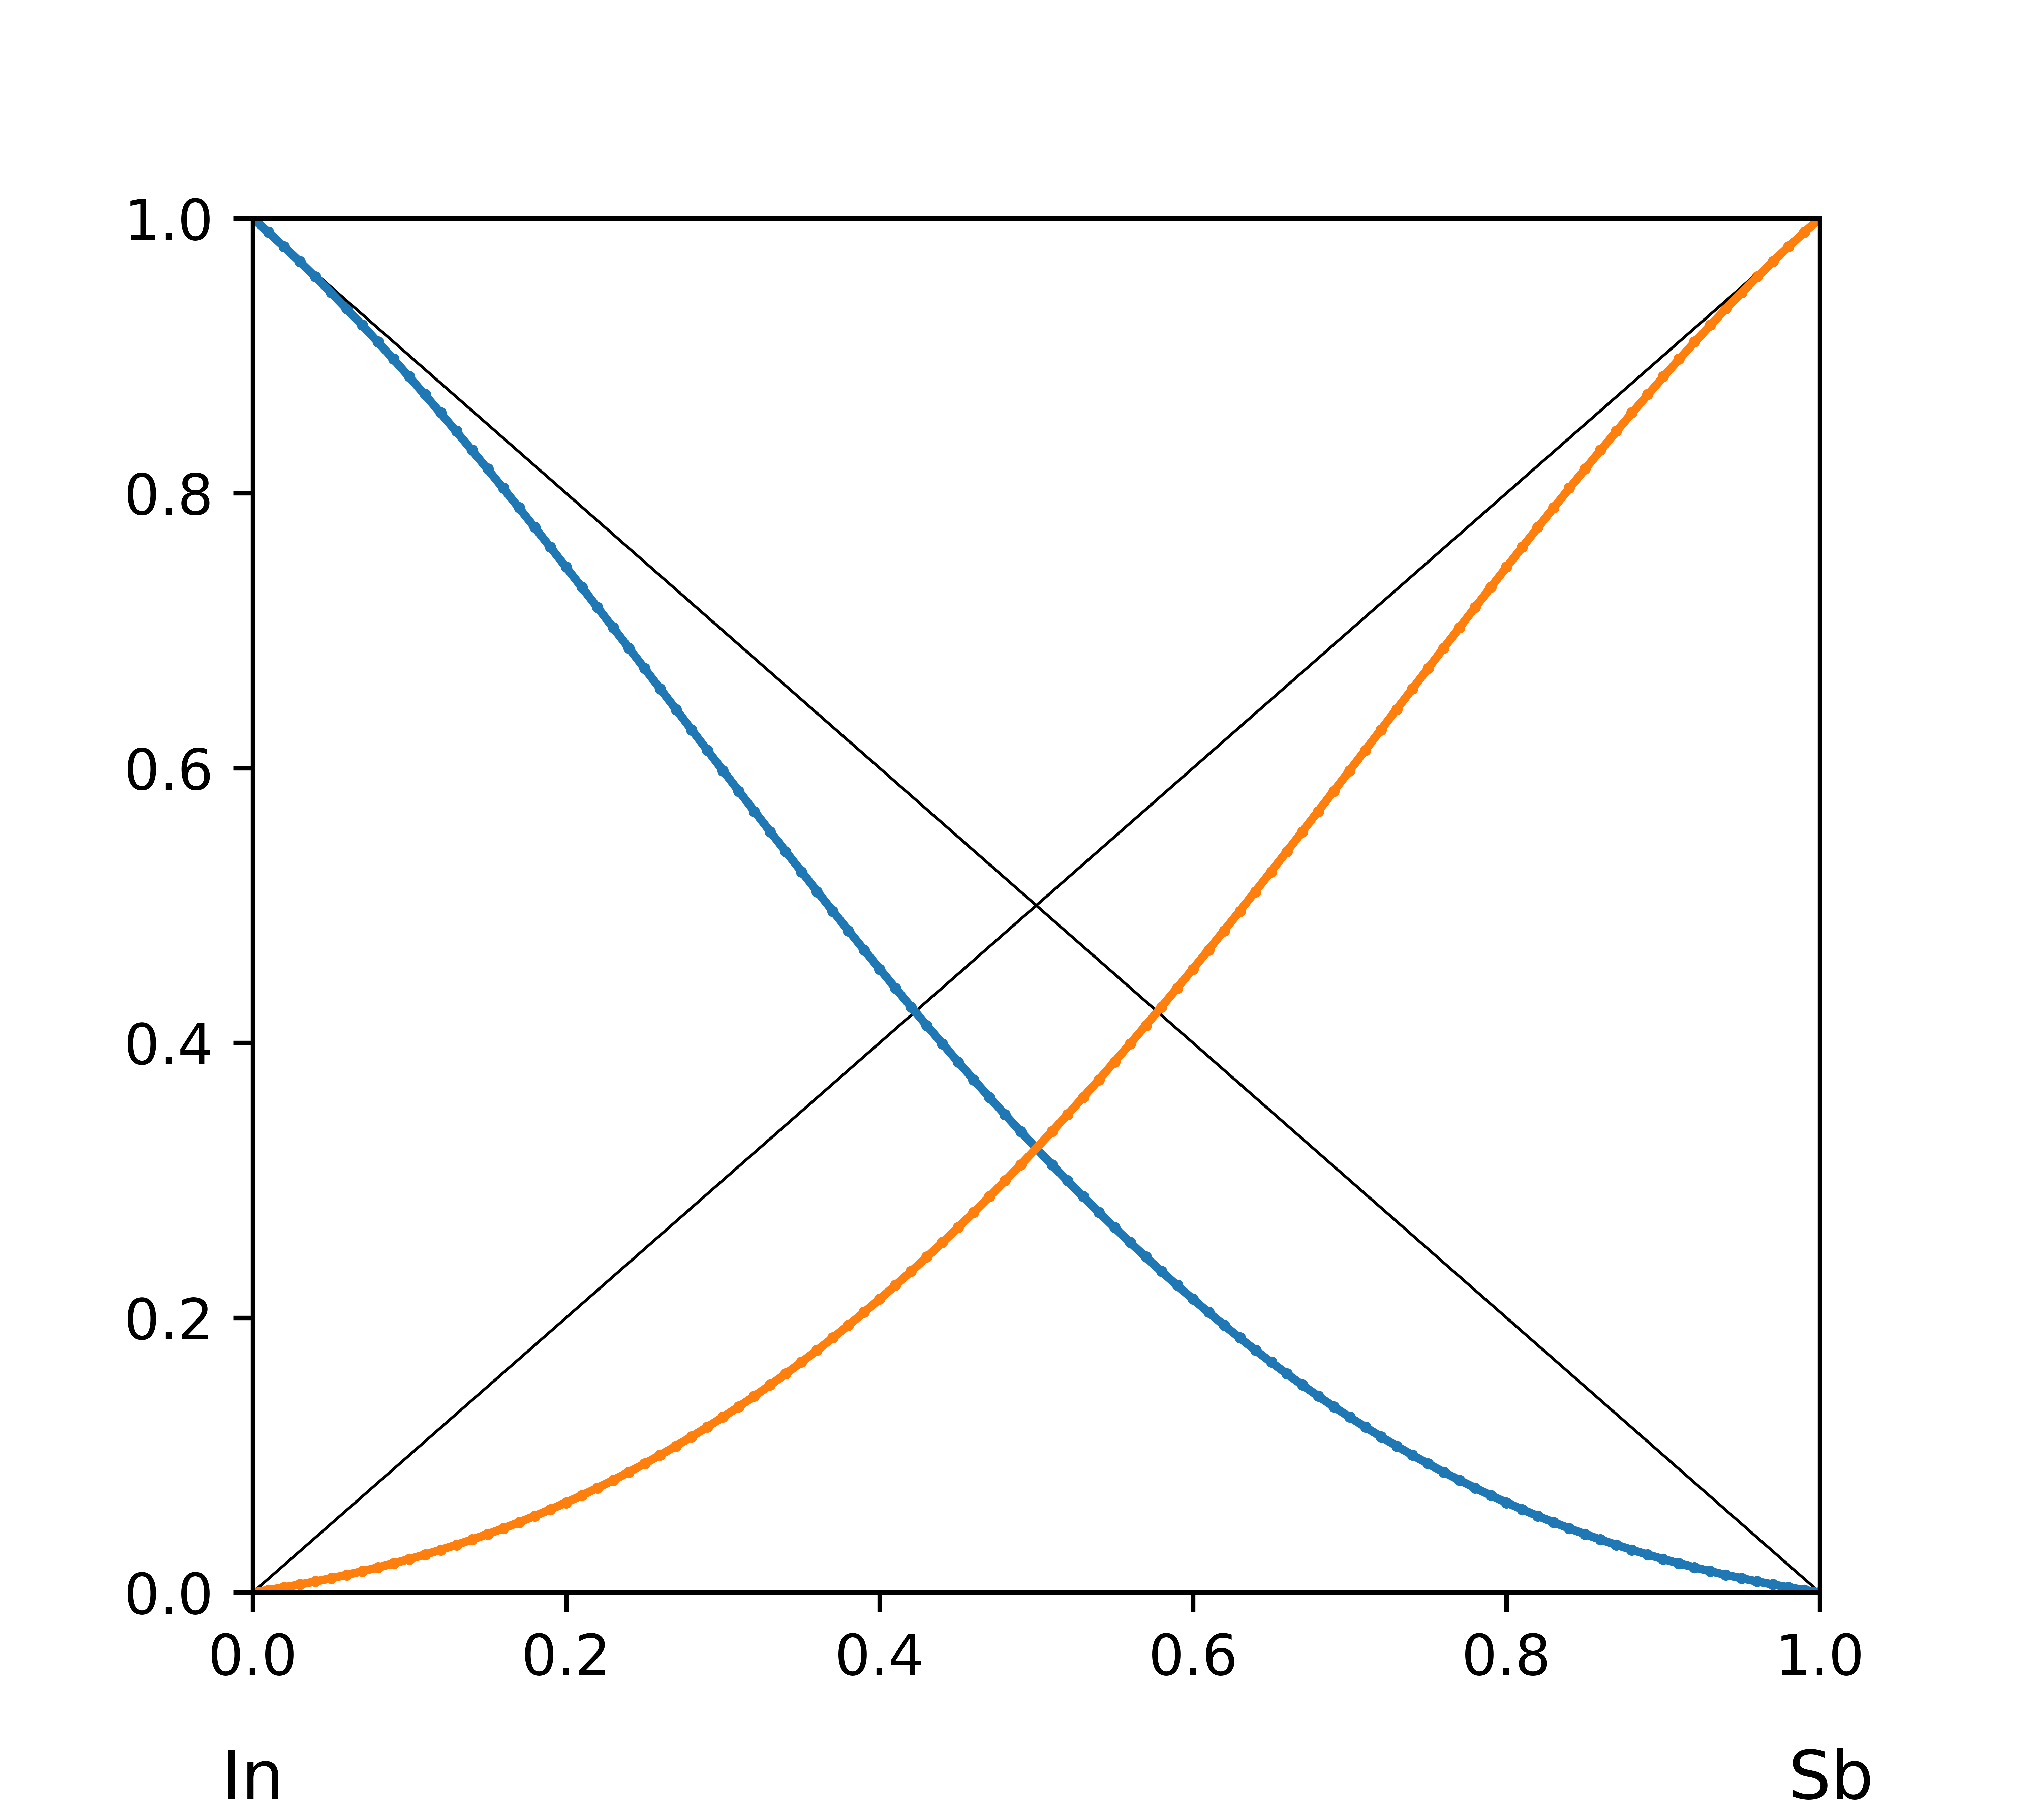
\includegraphics[width=1\linewidth]{In-Sb_Activity}
  \caption{Component Activities}
  \label{fig:sub1}
\end{subfigure}%
\begin{subfigure}{.5\textwidth}
  \centering
  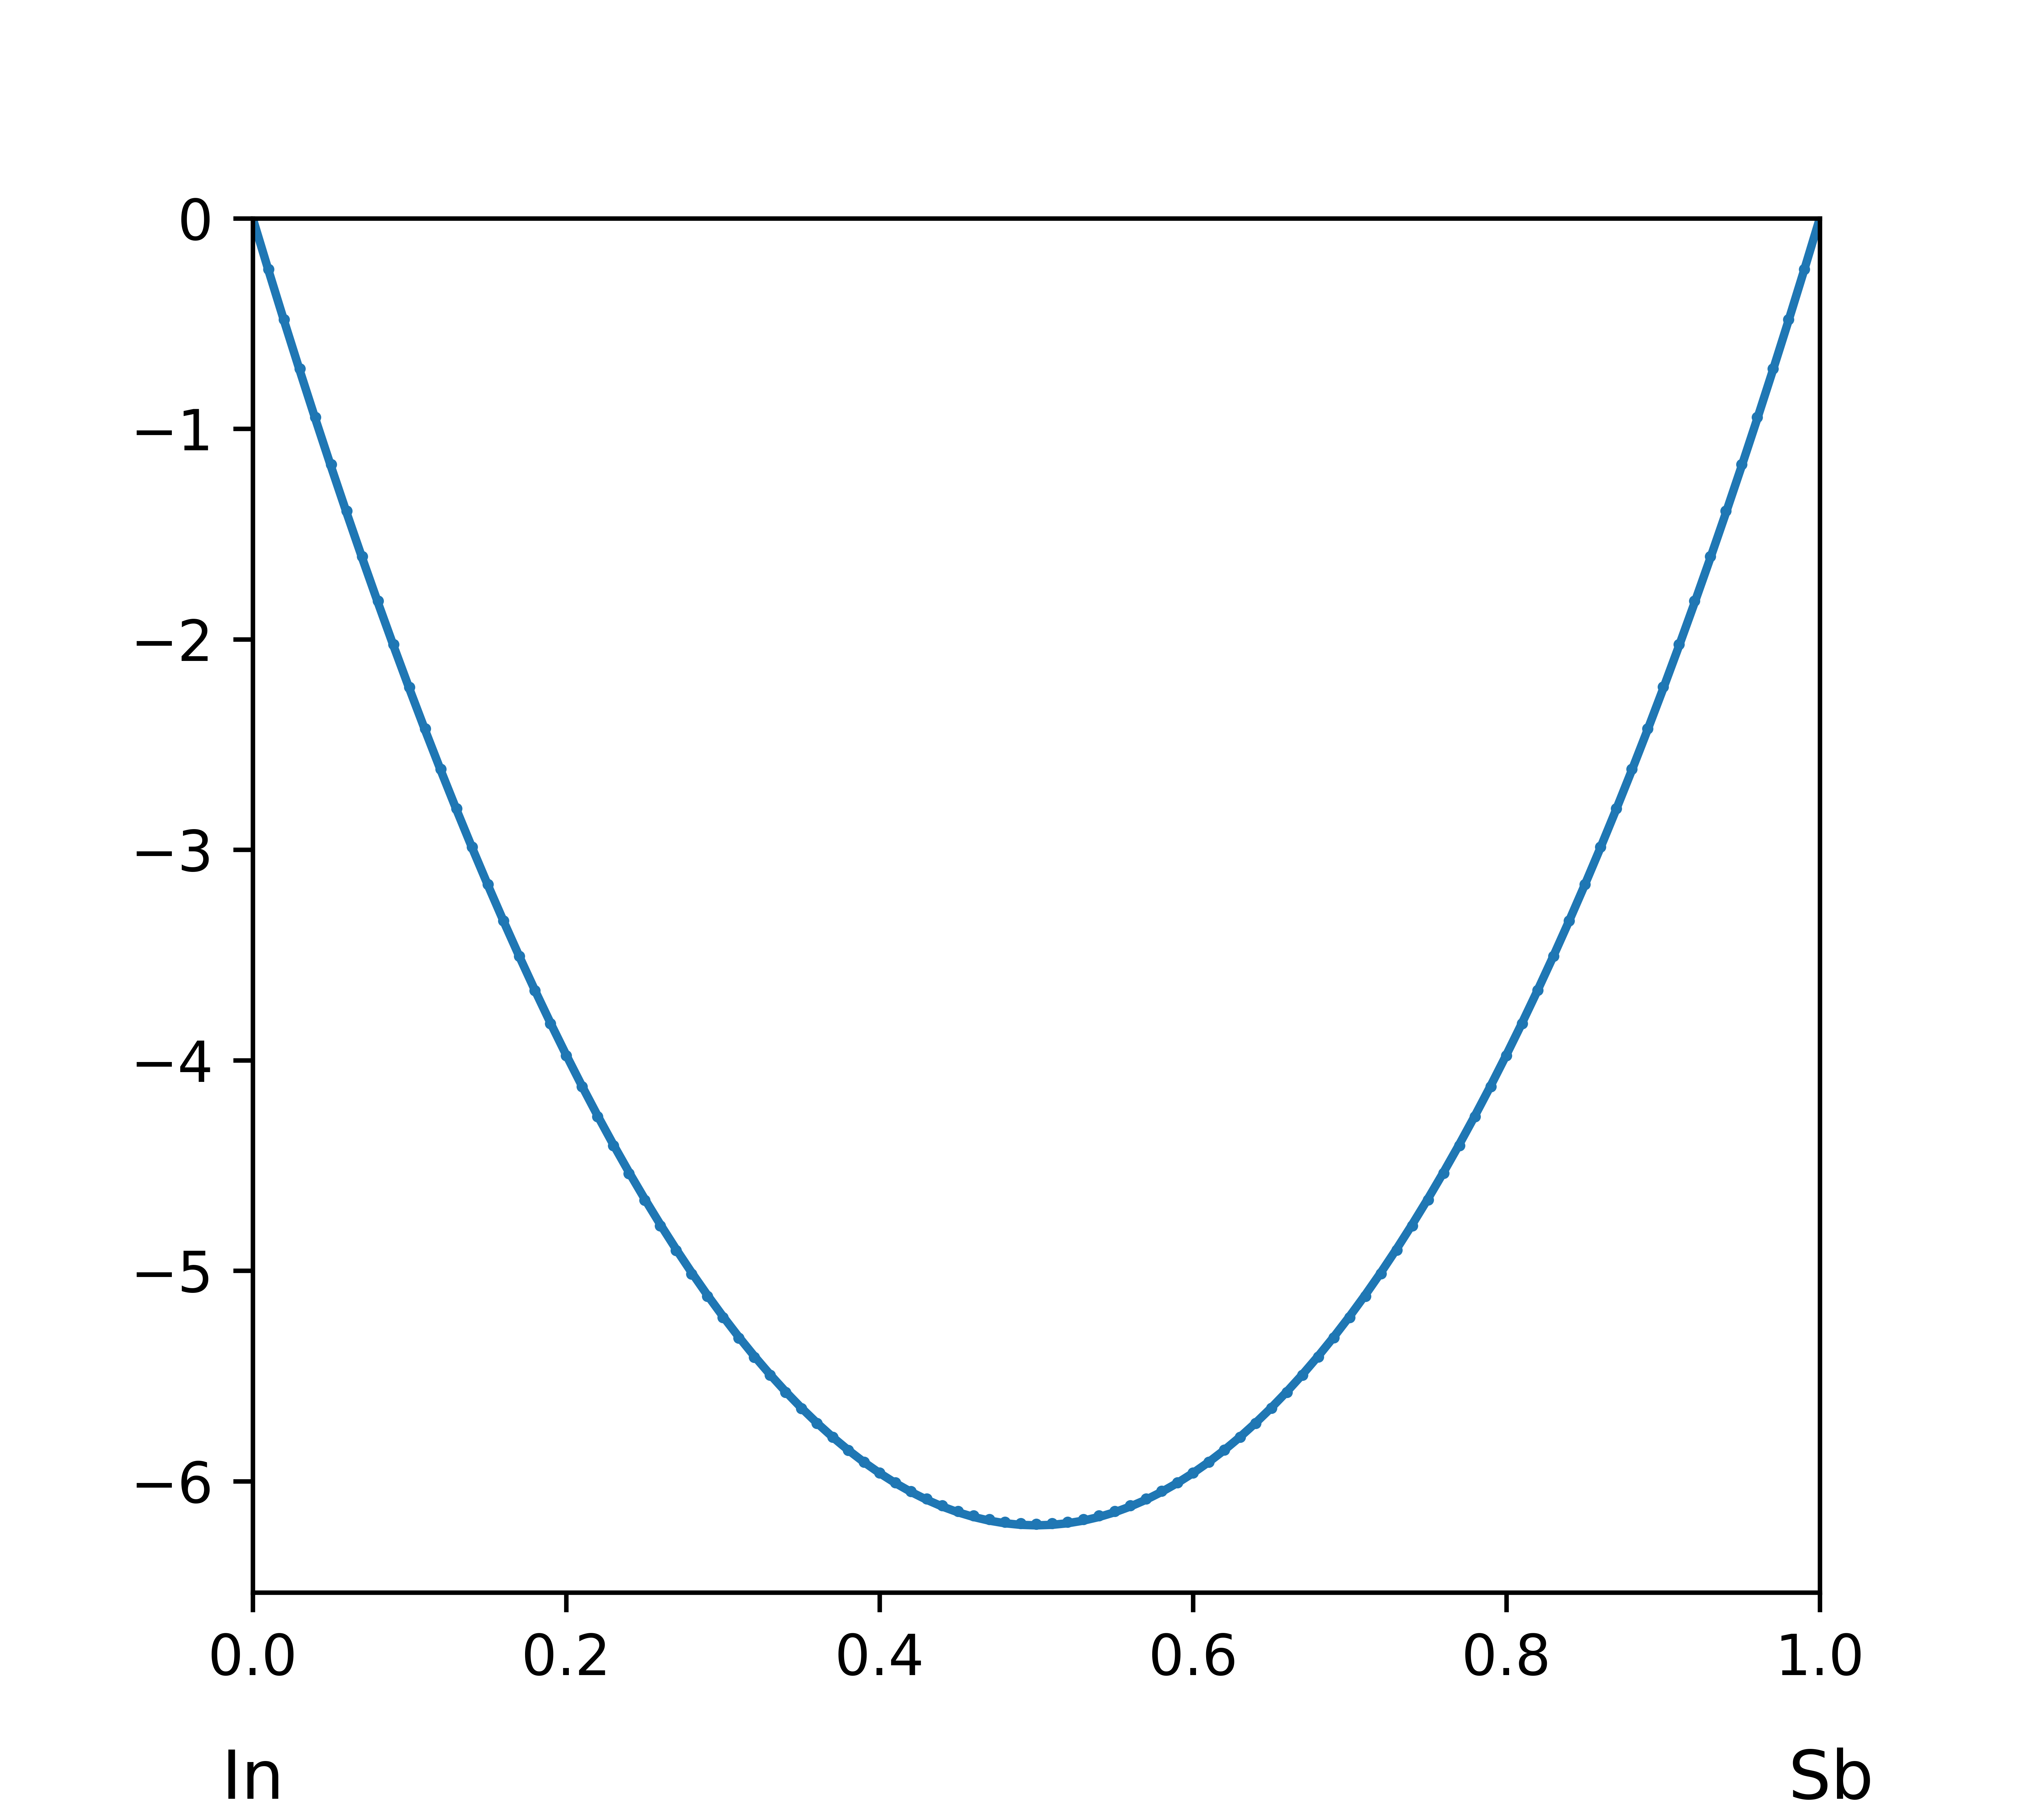
\includegraphics[width=1\linewidth]{In-Sb_Enthalpy}
  \caption{Enthalpy of Mixing (kJ/mol)}
  \label{fig:sub2}
\end{subfigure}
\caption{System In-Sb (T = 1200 K): solid lines -- \cite{Ag-In_Data}; dotted lines - TISR}
\label{fig:In-Sb}
\end{figure}

\begin{figure}
\centering
\begin{subfigure}{.5\textwidth}
  \centering
  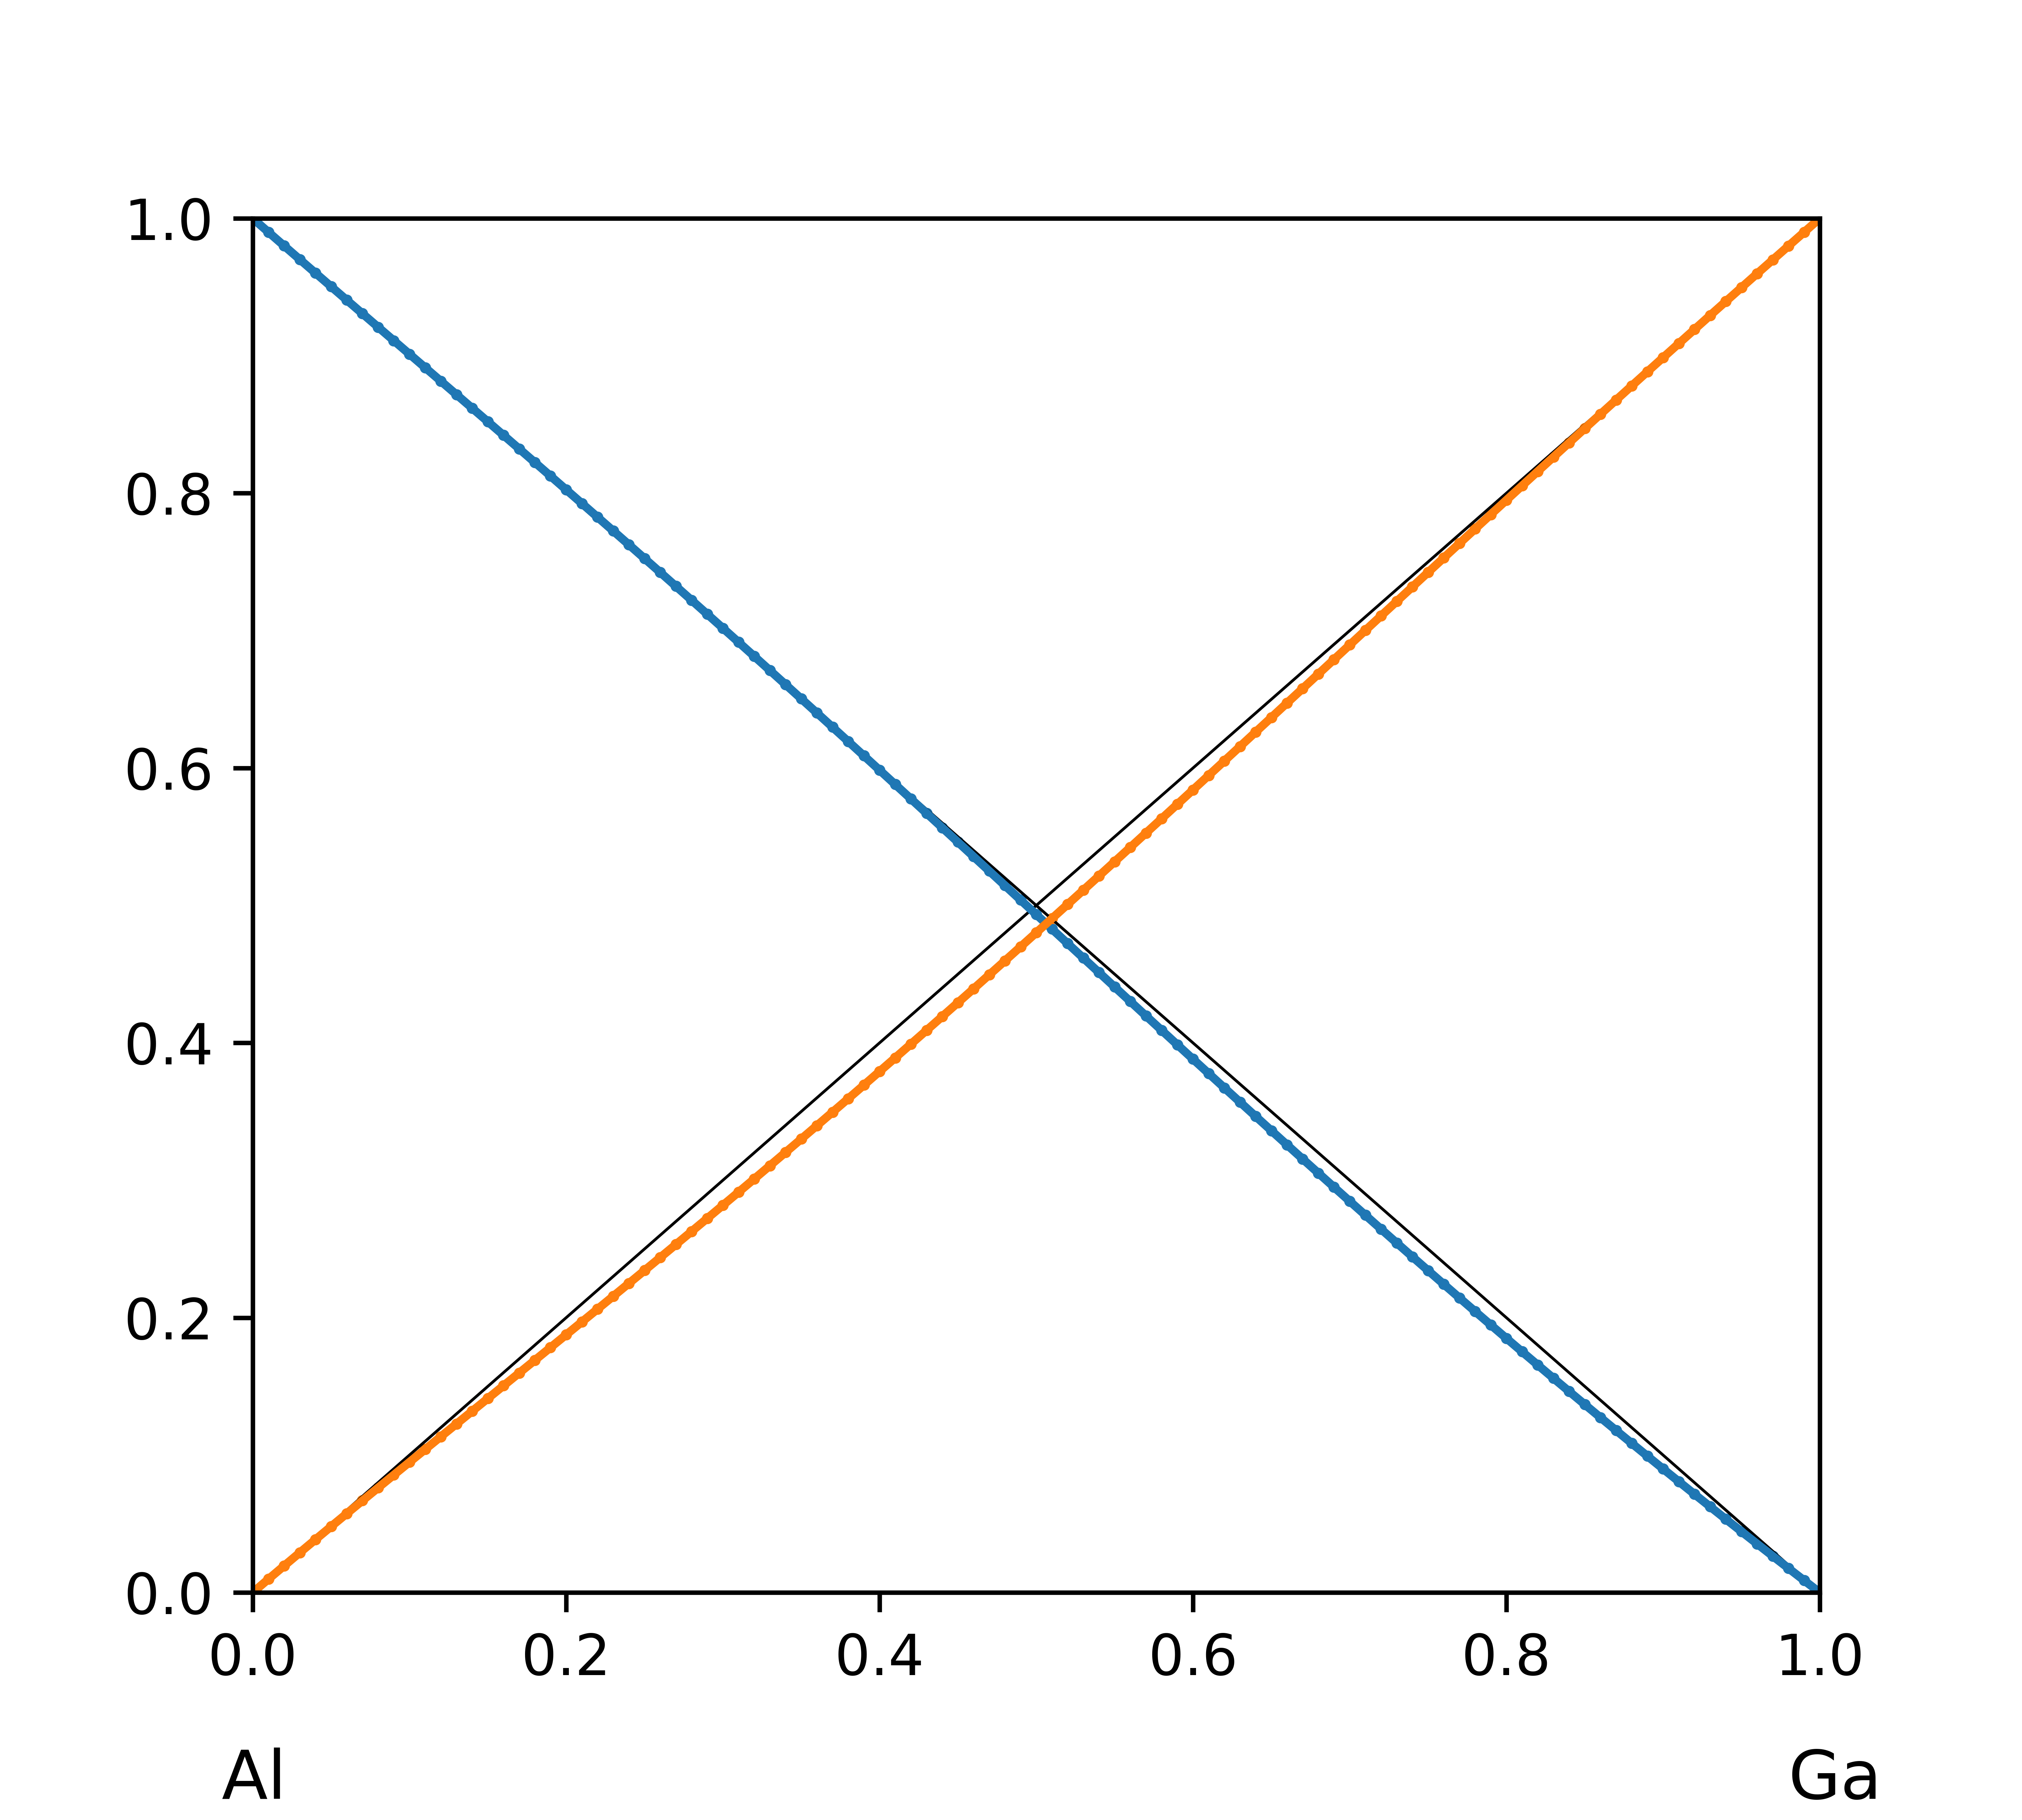
\includegraphics[width=1\linewidth]{Al-Ga_Activity}
  \caption{Component Activities}
  \label{fig:sub1}
\end{subfigure}%
\begin{subfigure}{.5\textwidth}
  \centering
  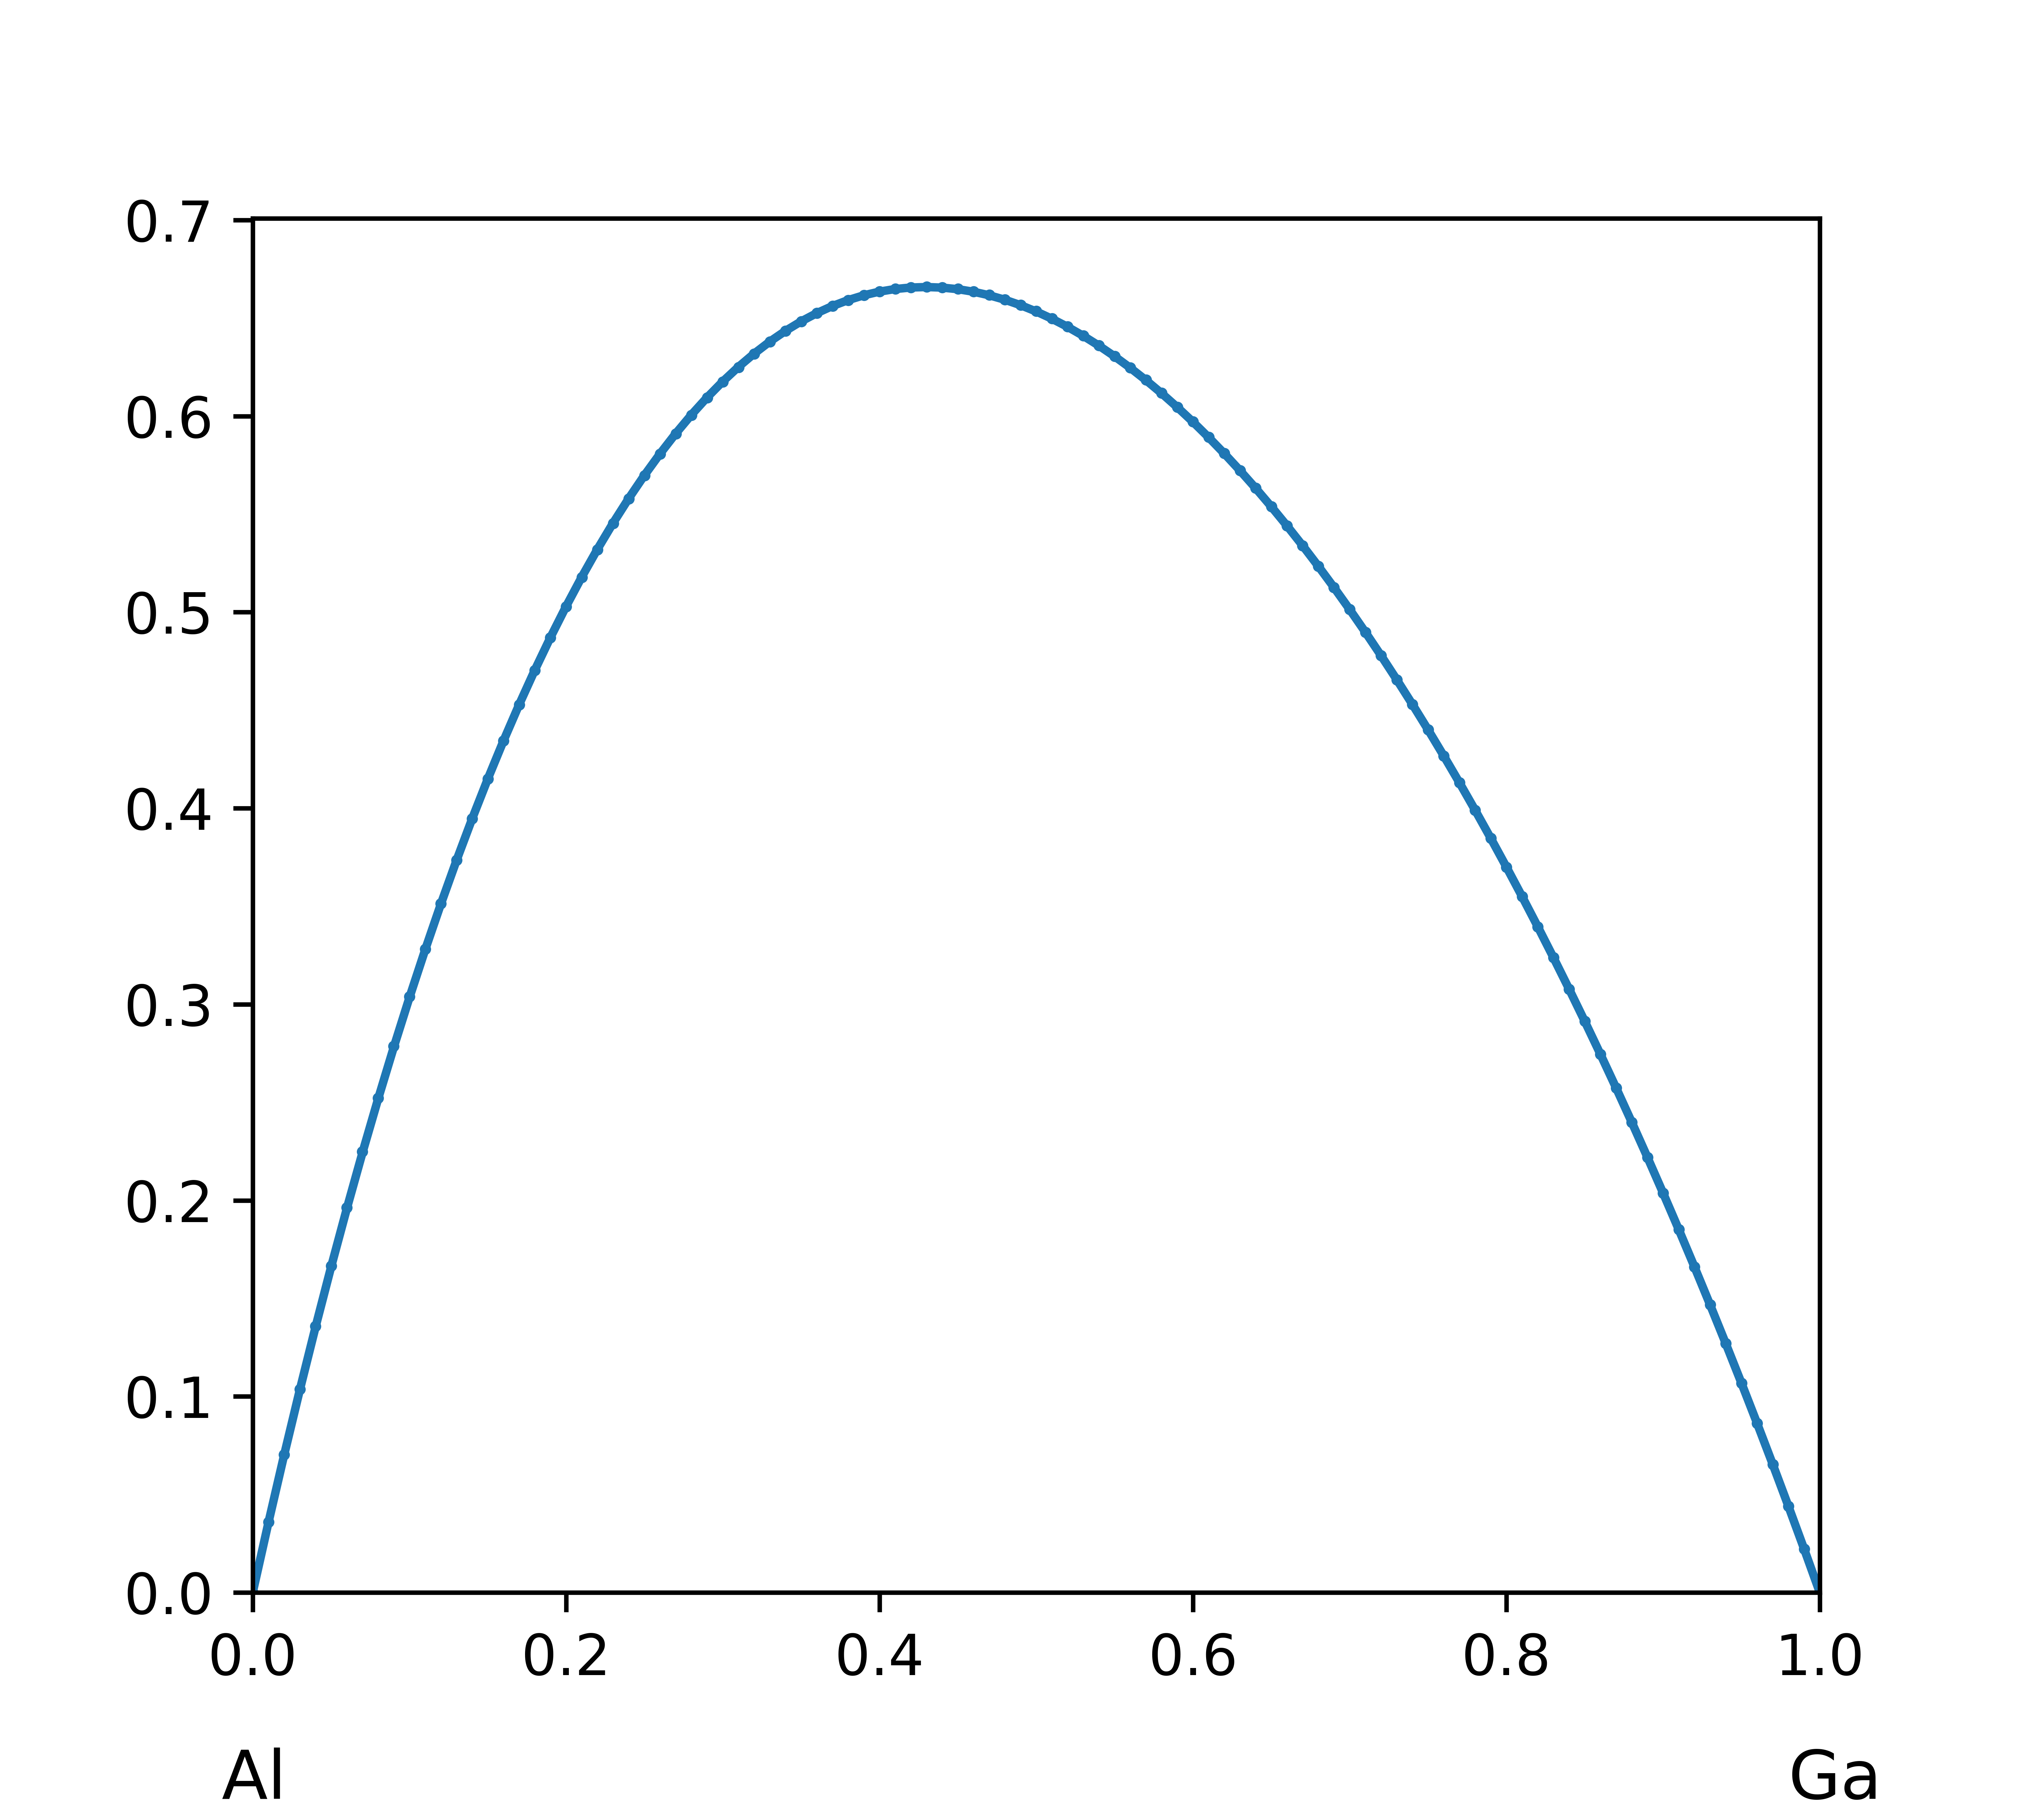
\includegraphics[width=1\linewidth]{Al-Ga_Enthalpy}
  \caption{Enthalpy of Mixing (kJ/mol)}
  \label{fig:sub2}
\end{subfigure}
\caption{System Al-Ga (T = 1273 K): solid lines -- \cite{Al-Ga_Data}; dotted lines - TISR}
\label{fig:Al-Ga}
\end{figure}

\begin{figure}
\centering
\begin{subfigure}{.5\textwidth}
  \centering
  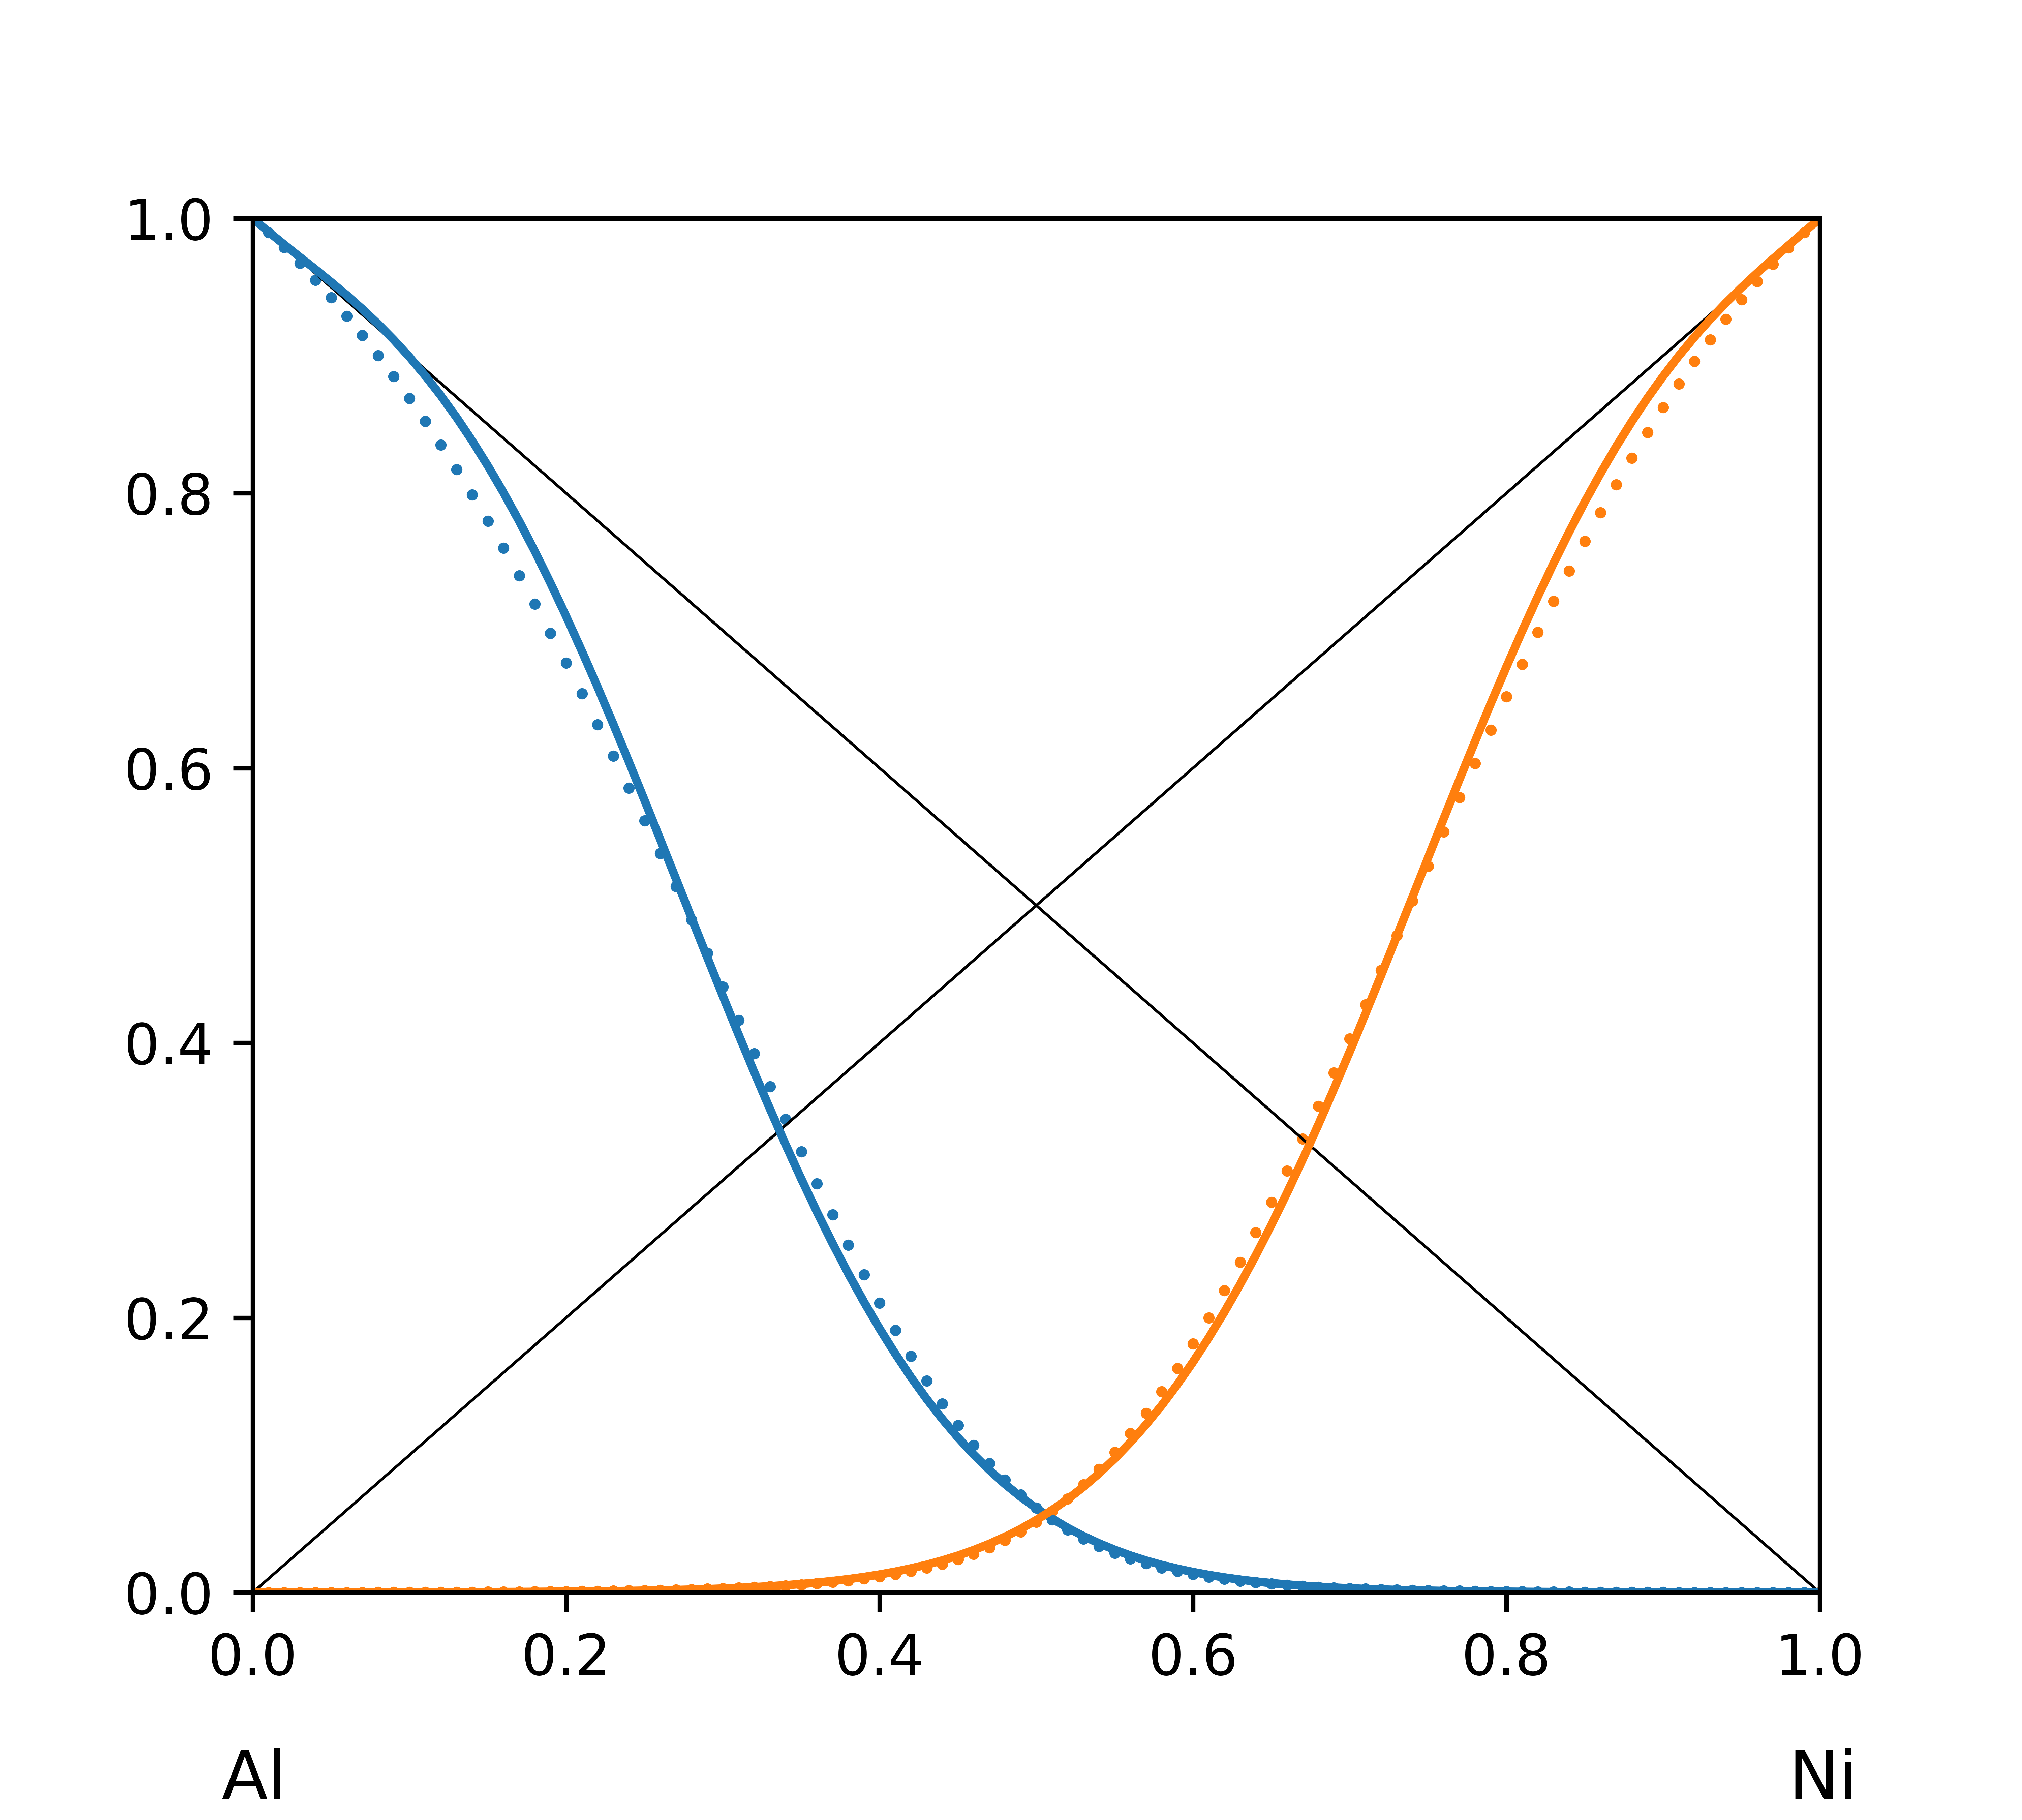
\includegraphics[width=1\linewidth]{Al-Ni_Activity}
  \caption{Component Activities}
  \label{fig:sub1}
\end{subfigure}%
\begin{subfigure}{.5\textwidth}
  \centering
  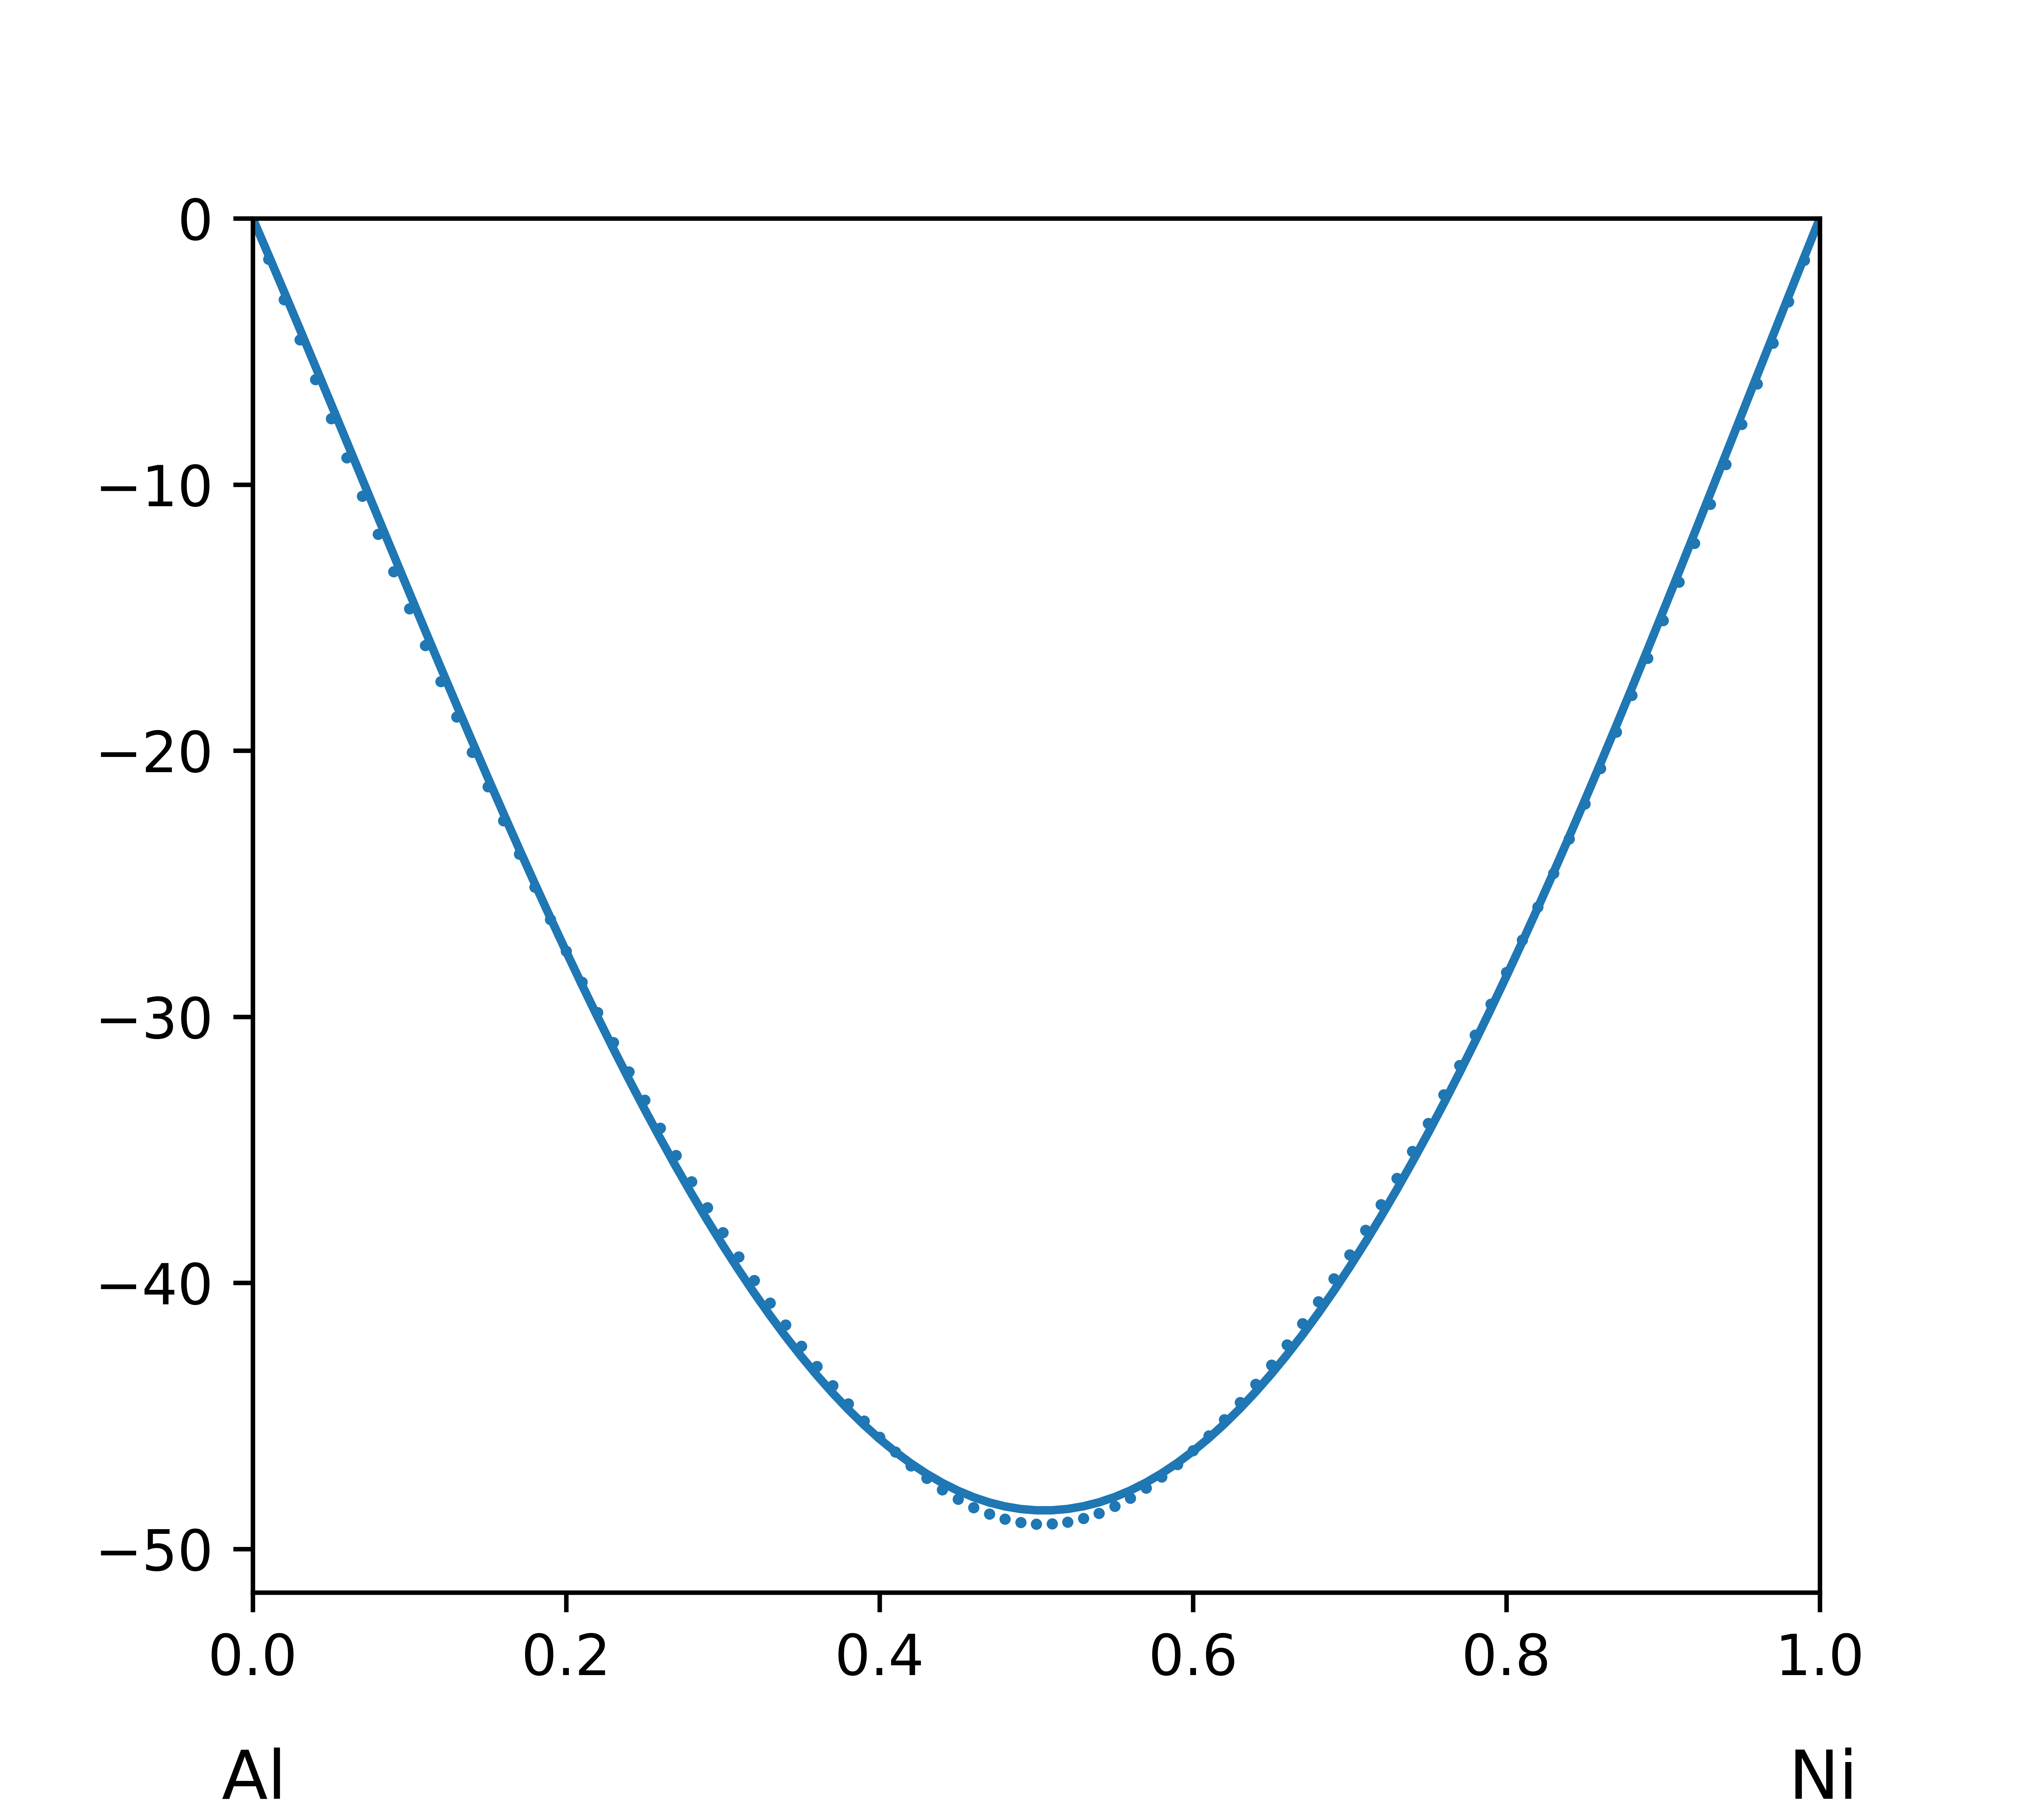
\includegraphics[width=1\linewidth]{Al-Ni_Enthalpy}
  \caption{Enthalpy of Mixing (kJ/mol)}
  \label{fig:sub2}
\end{subfigure}
\caption{System Al-Ni (T = 1923 K): solid lines -- \cite{Al-Ni_Data}; dotted lines - TISR}
\label{fig:Al-Ni}
\end{figure}

\begin{figure}
\centering
\begin{subfigure}{.5\textwidth}
  \centering
  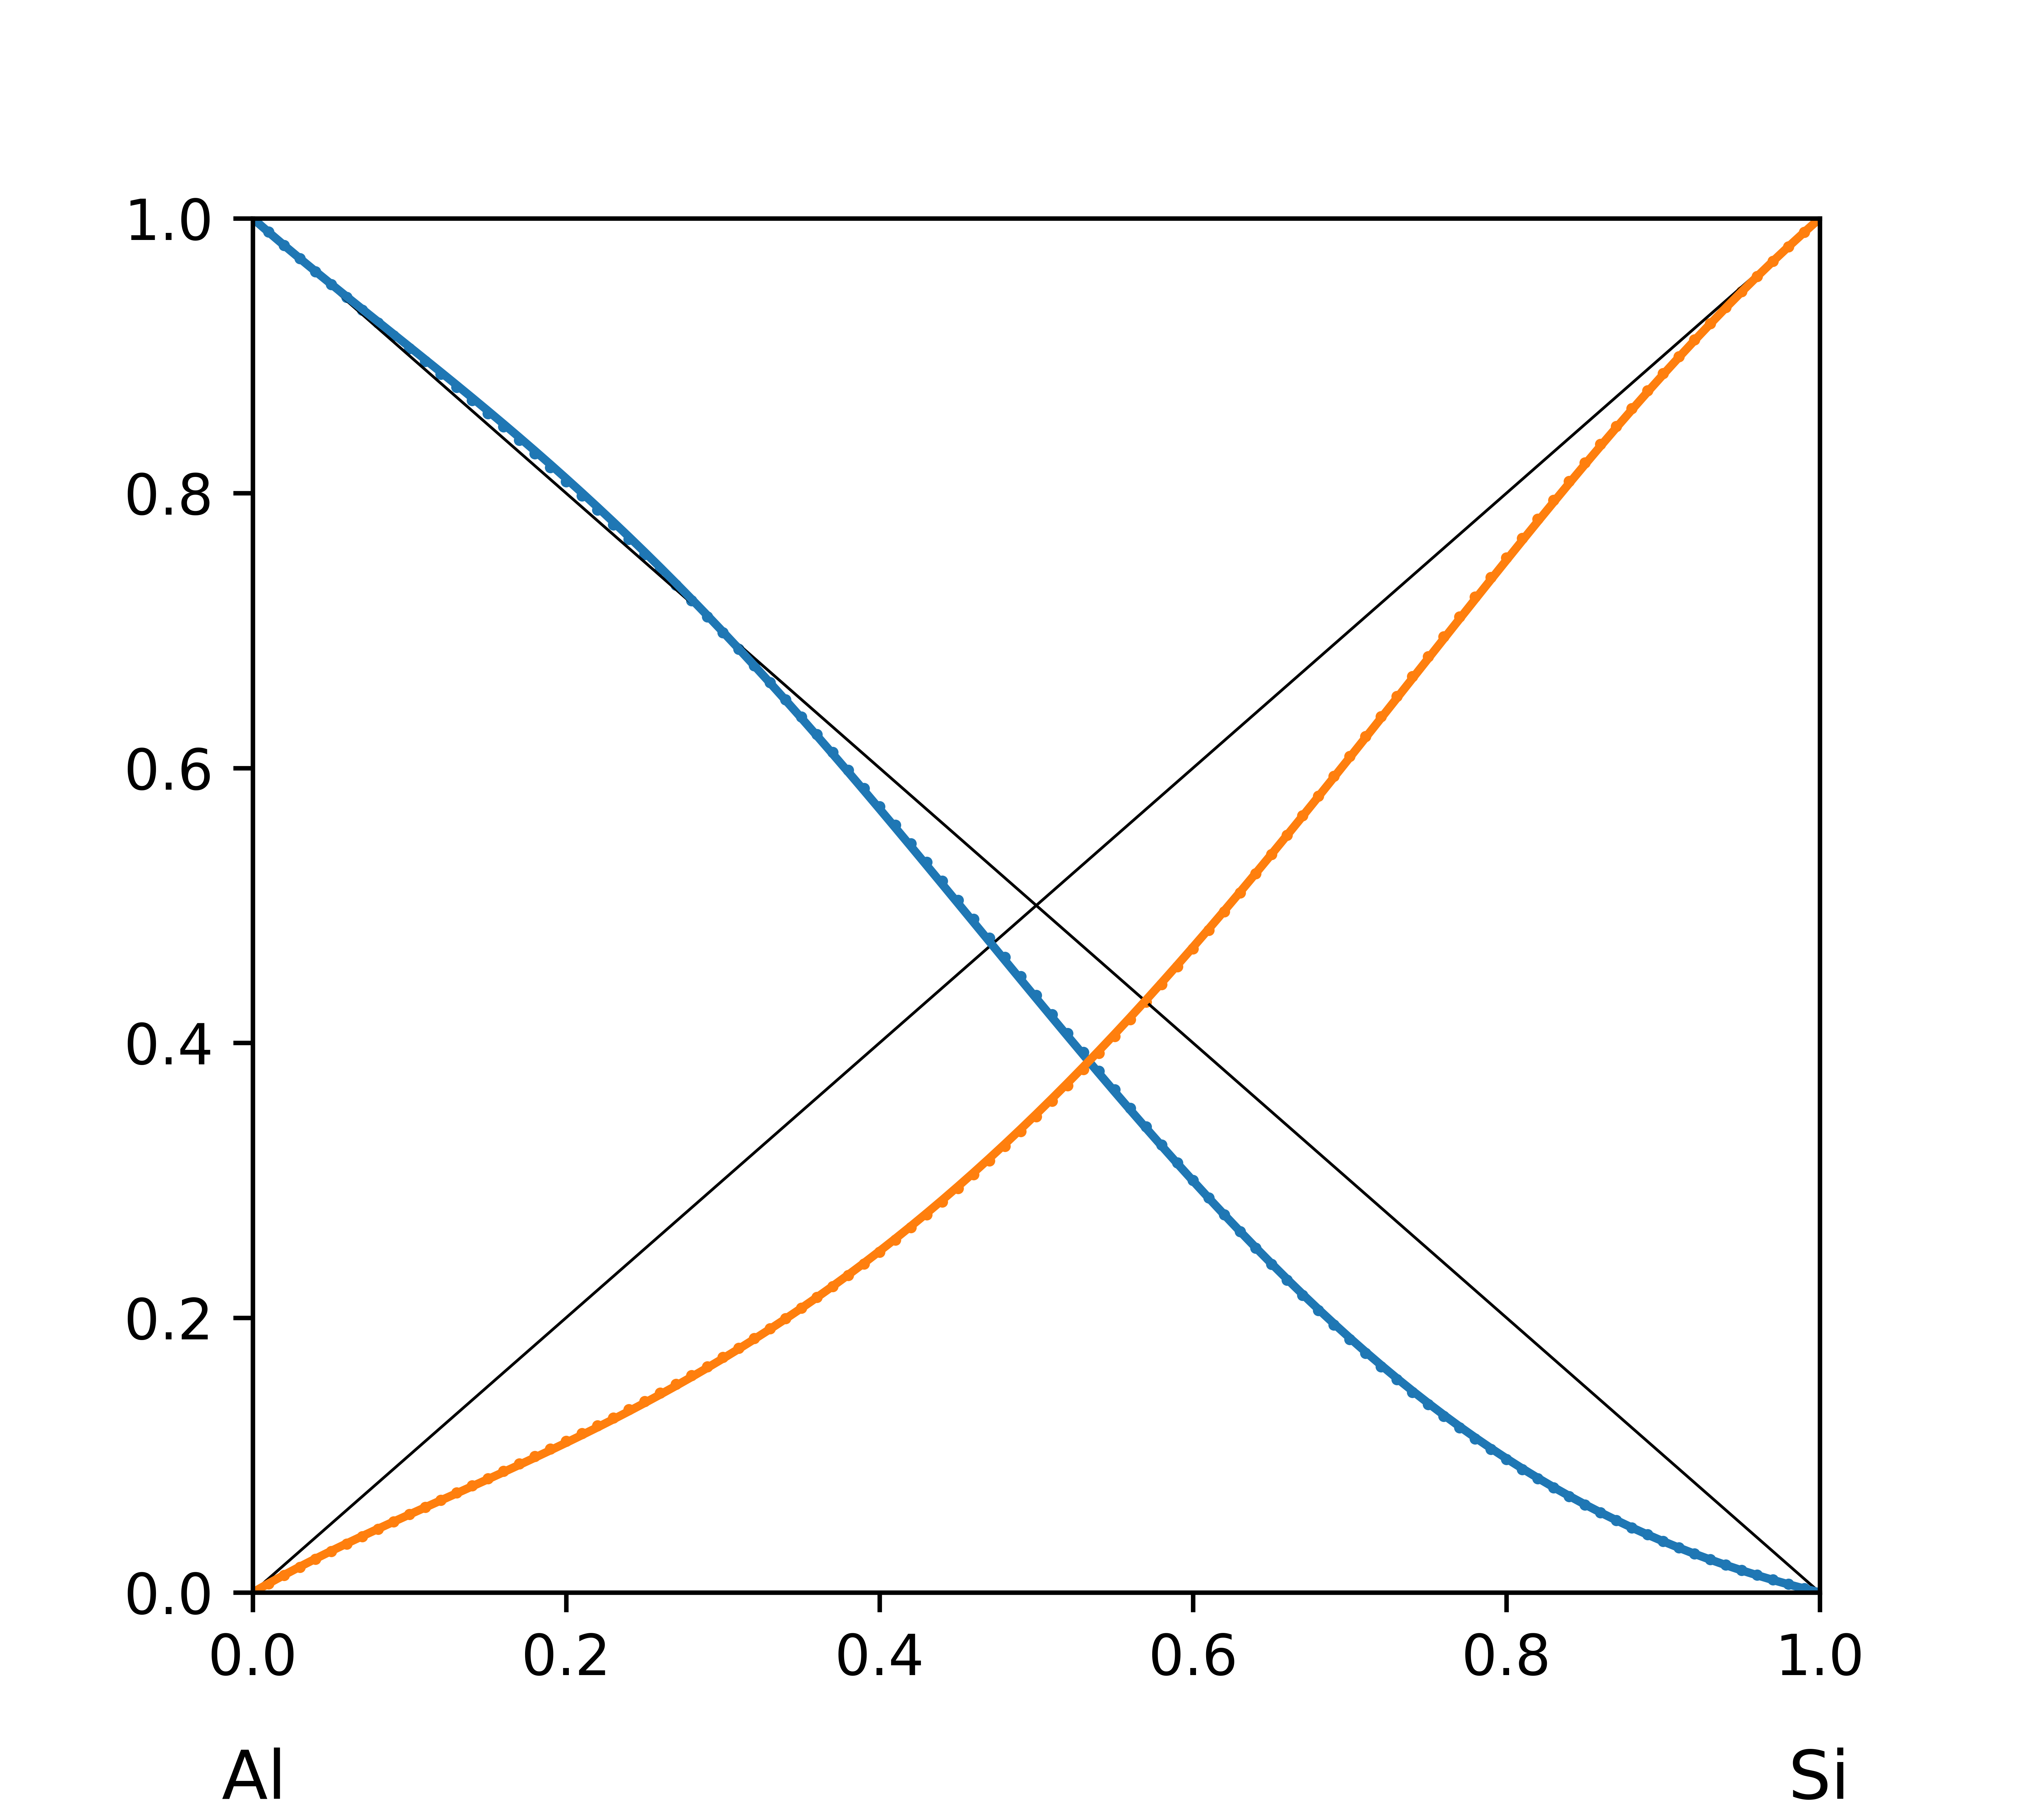
\includegraphics[width=1\linewidth]{Al-Si_Activity}
  \caption{Component Activities}
  \label{fig:sub1}
\end{subfigure}%
\begin{subfigure}{.5\textwidth}
  \centering
  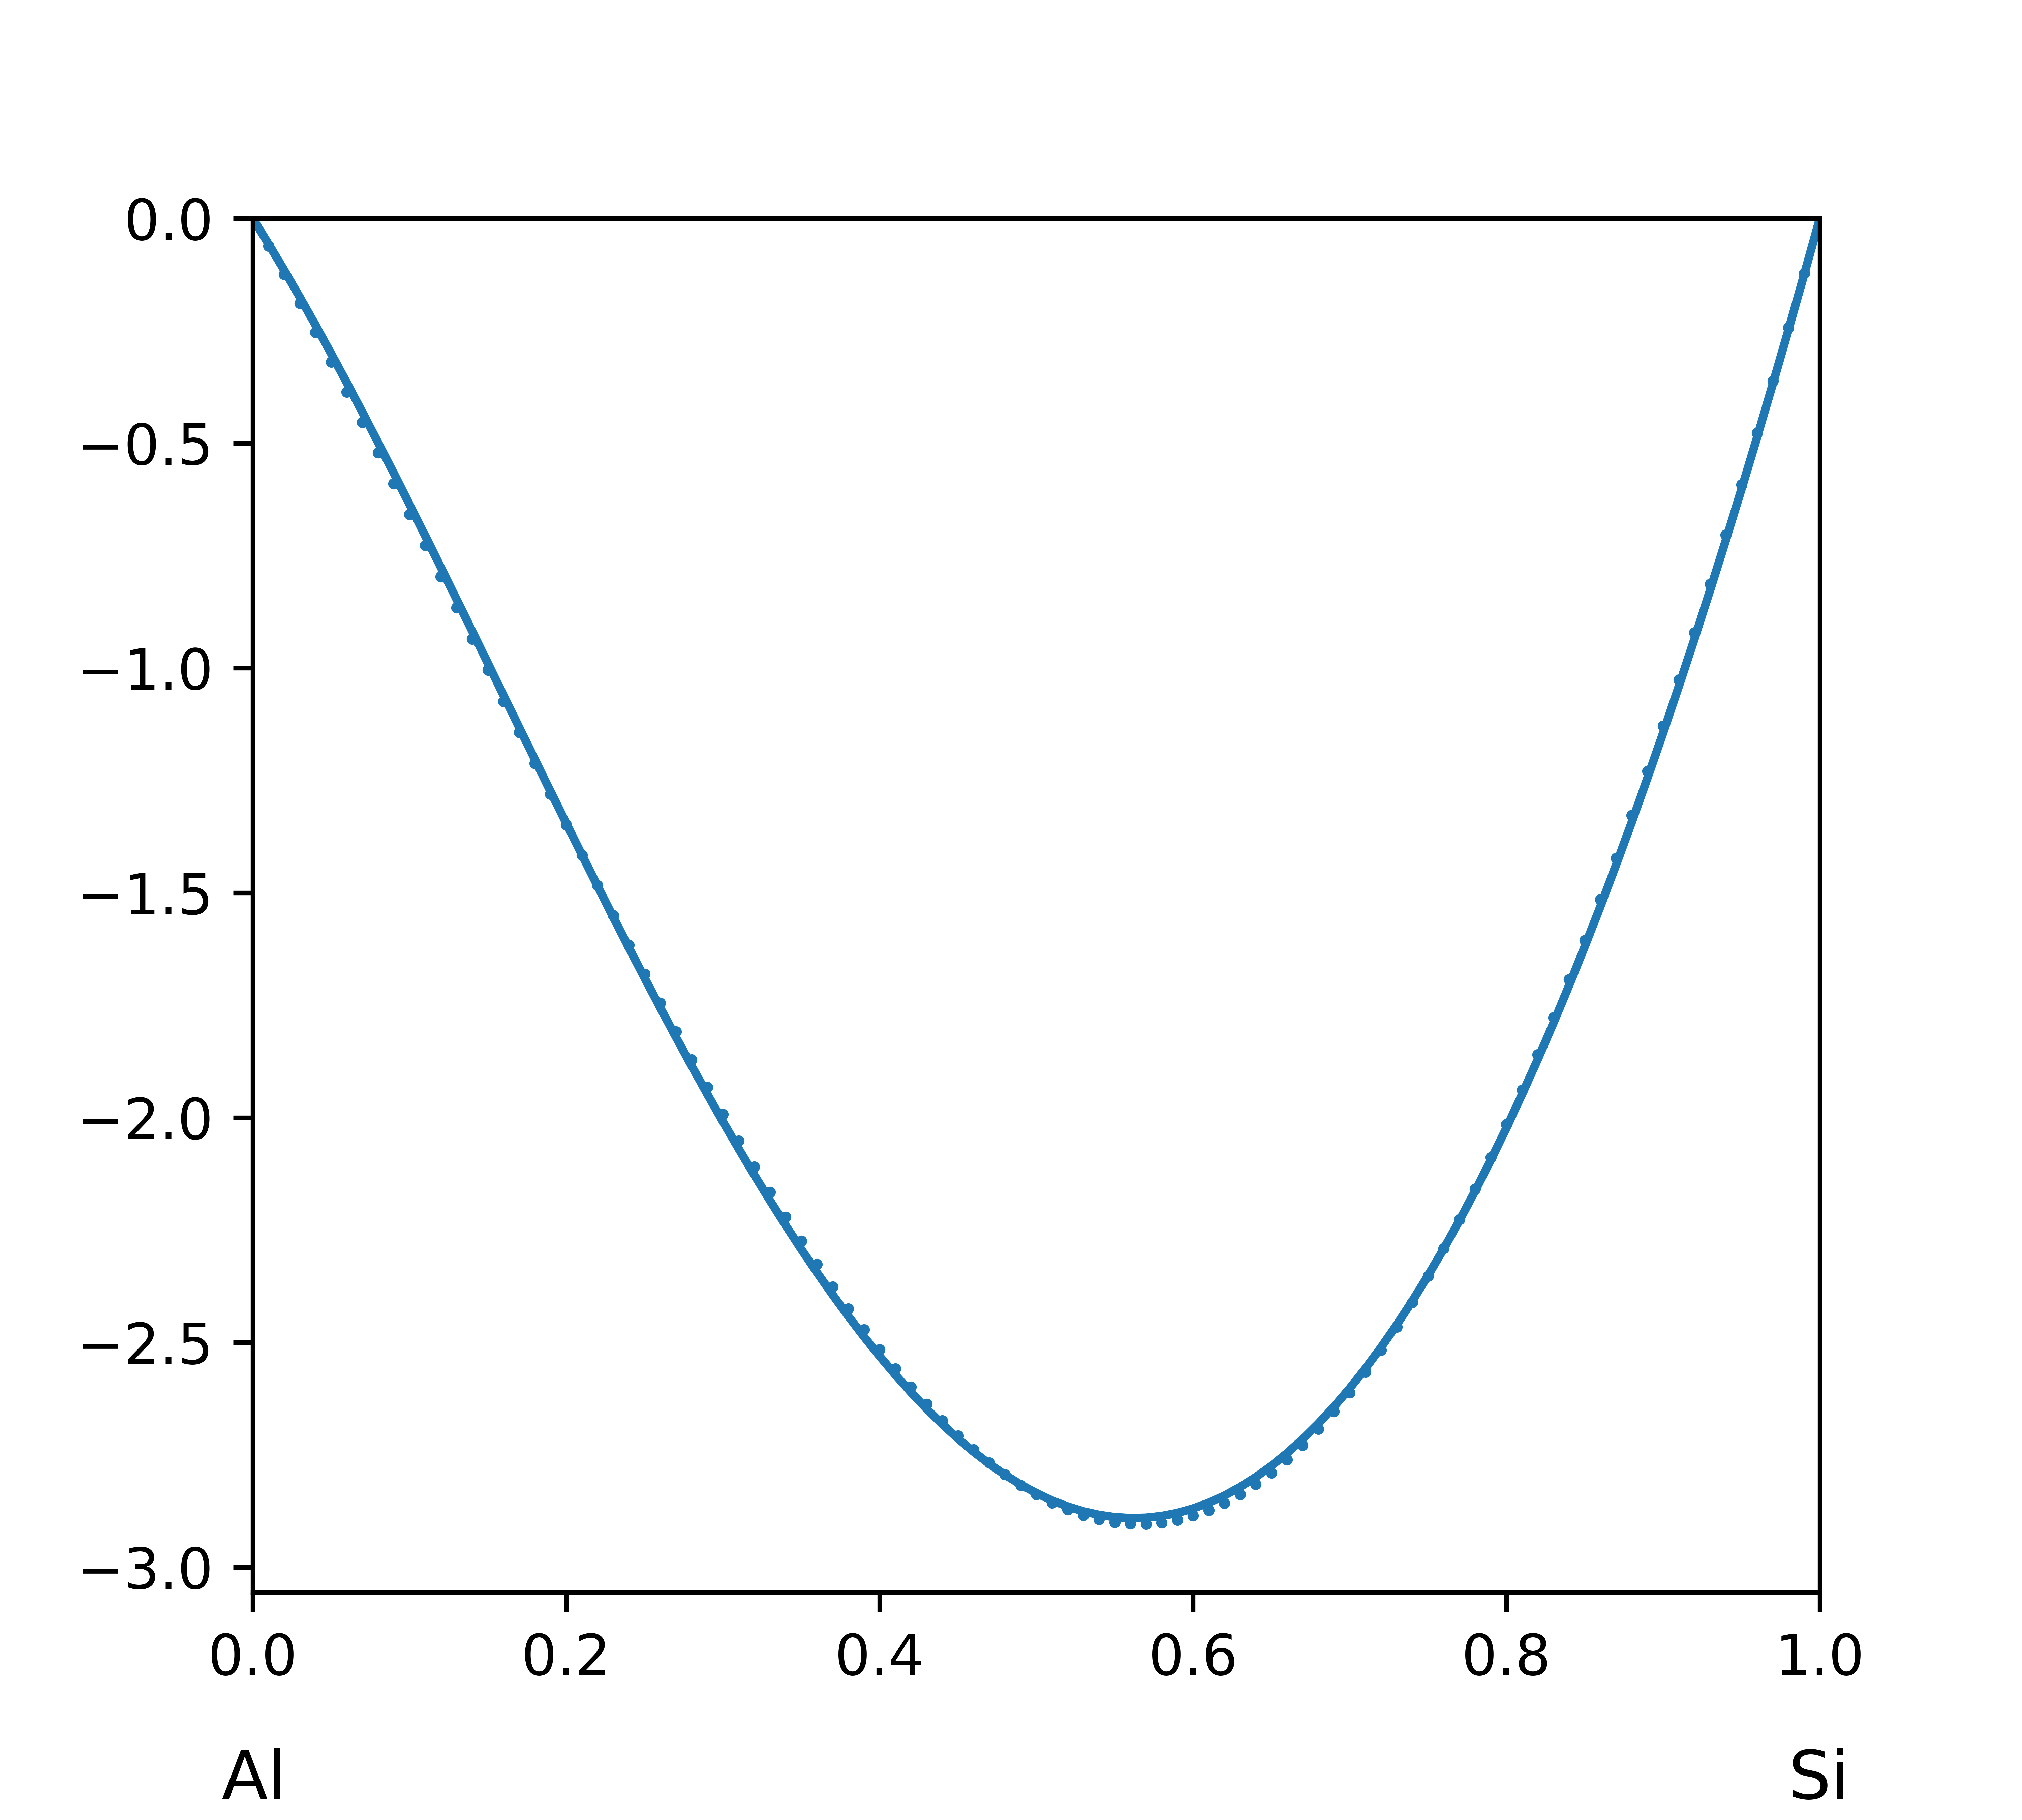
\includegraphics[width=1\linewidth]{Al-Si_Enthalpy}
  \caption{Enthalpy of Mixing (kJ/mol)}
  \label{fig:sub2}
\end{subfigure}
\caption{System Al-Si (T = 1575 K): solid lines -- \cite{Al-Si_Data}; dotted lines - TISR}
\label{fig:Al-Si} 
\end{figure}



\begin{figure}
\centering
\begin{subfigure}{.5\textwidth}
  \centering
  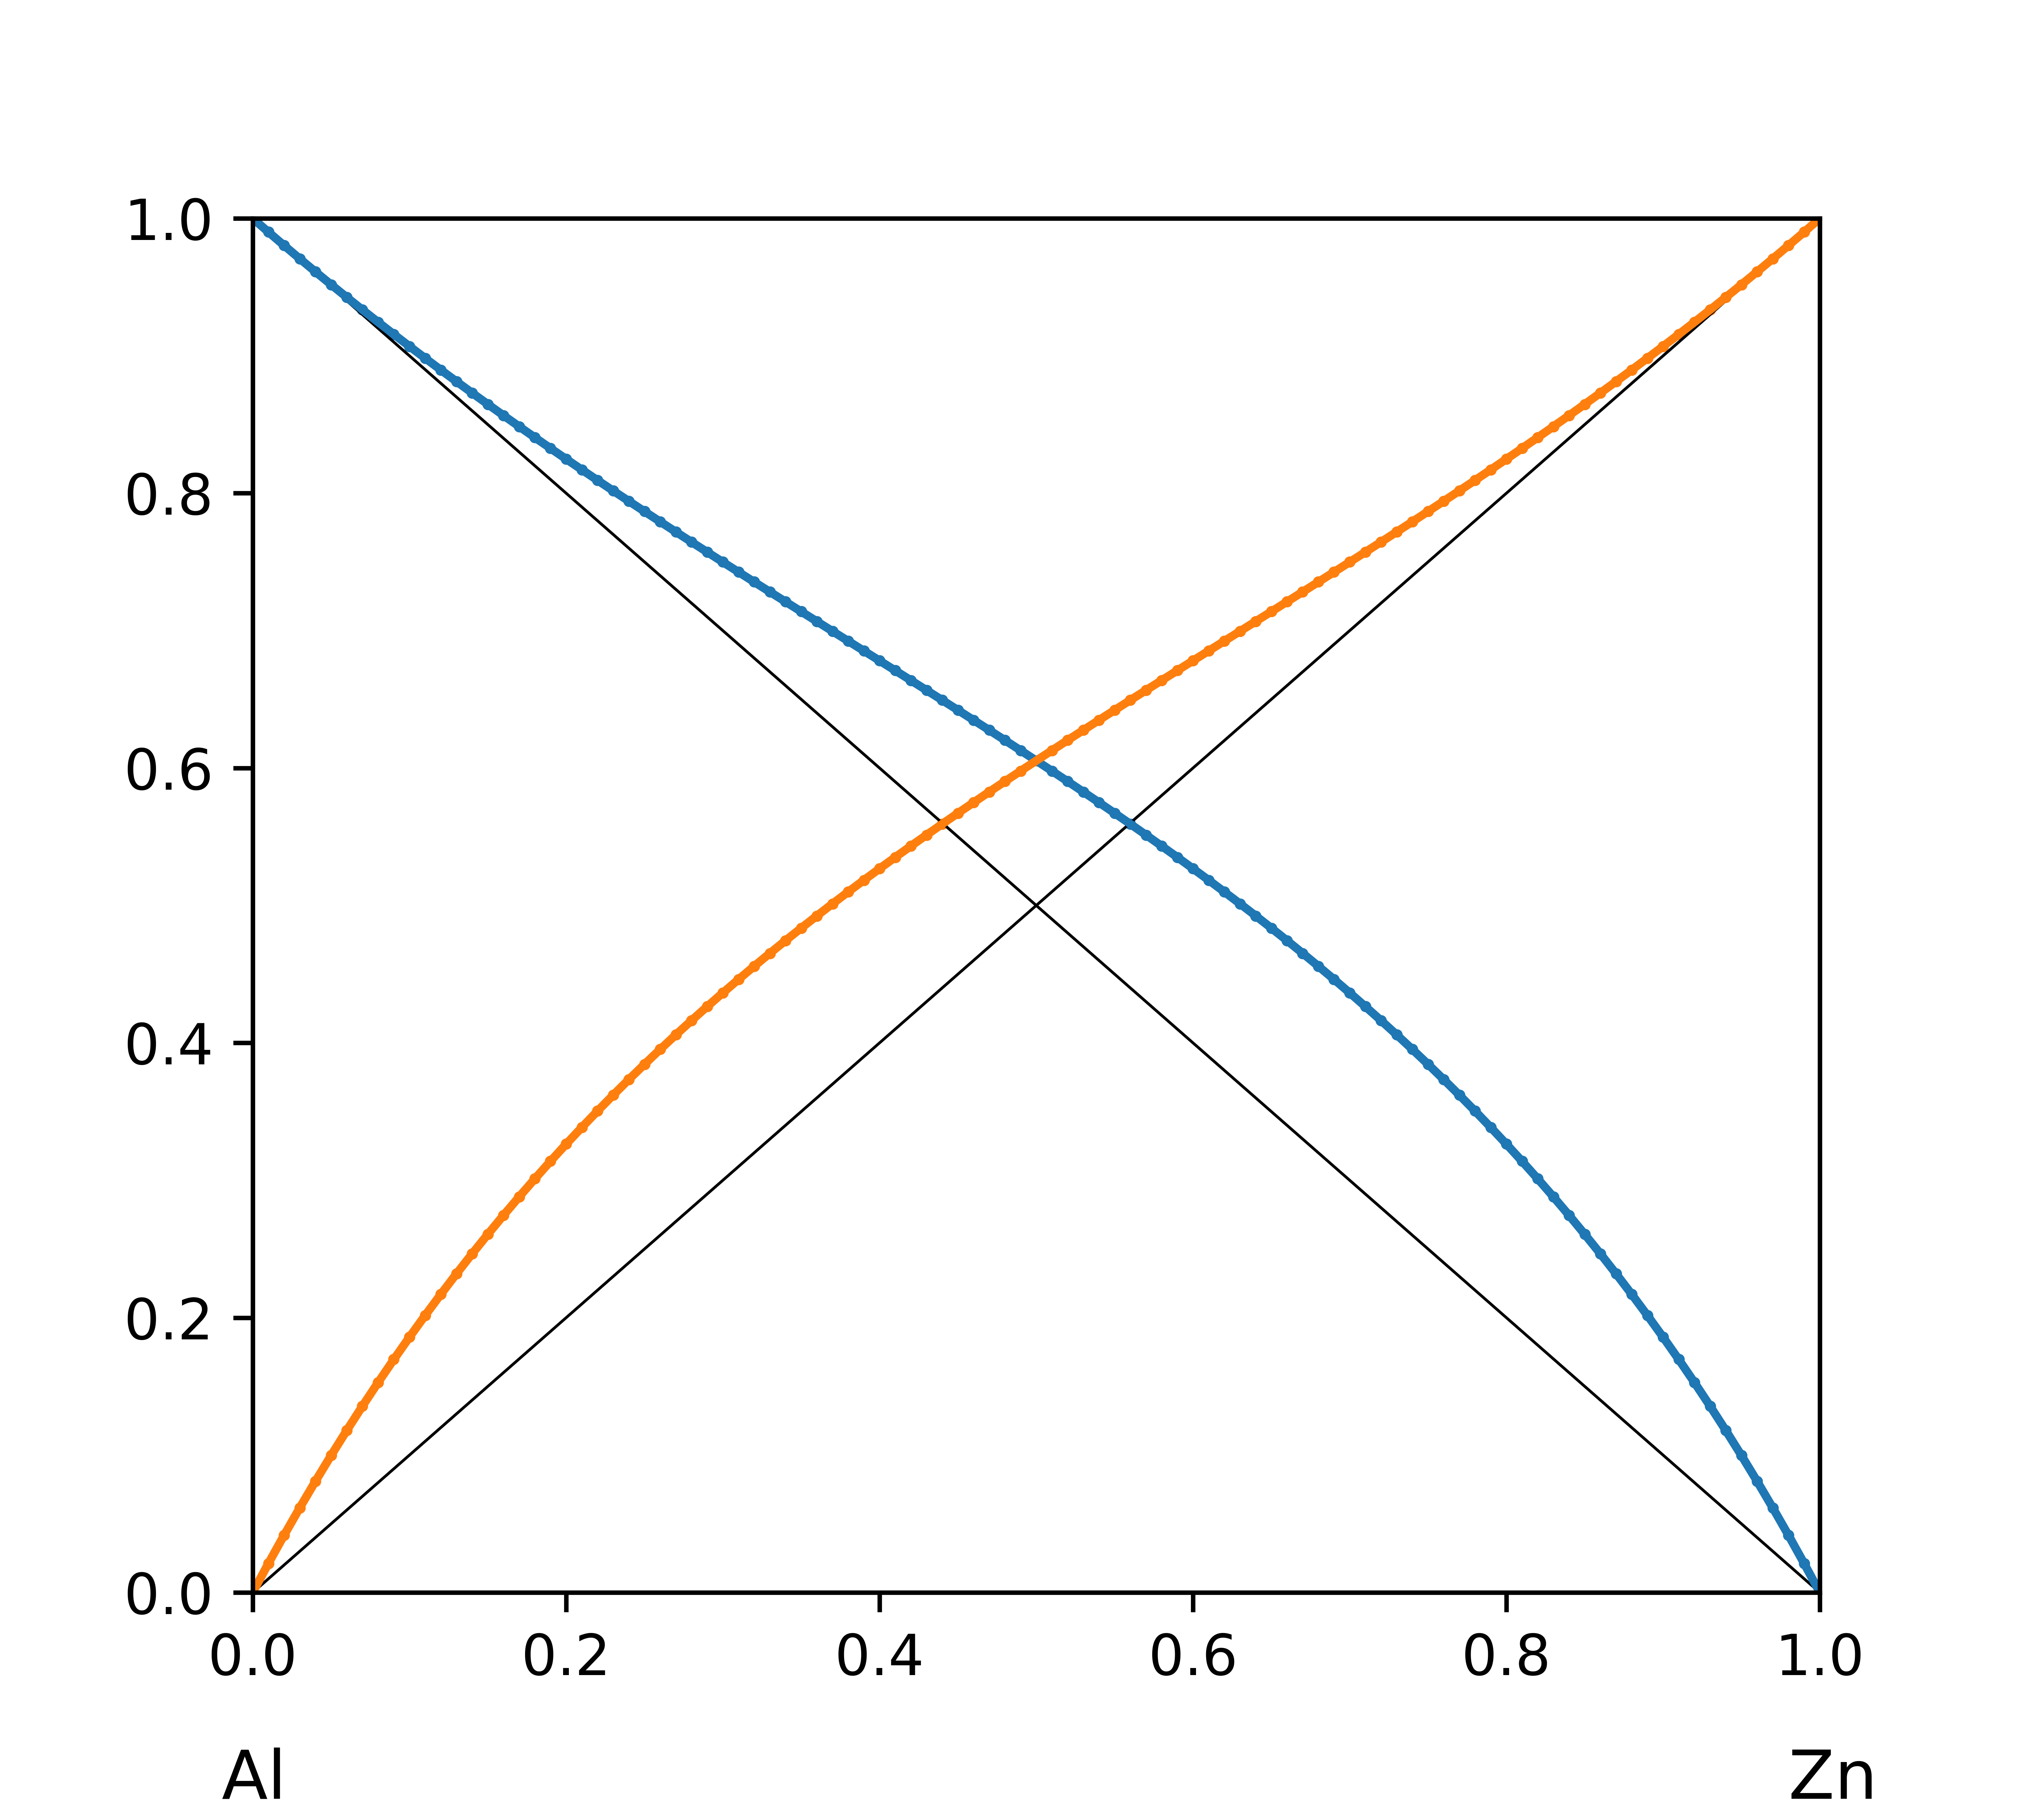
\includegraphics[width=1\linewidth]{Al-Zn_Activity}
  \caption{Component Activities}
  \label{fig:sub1}
\end{subfigure}%
\begin{subfigure}{.5\textwidth}
  \centering
  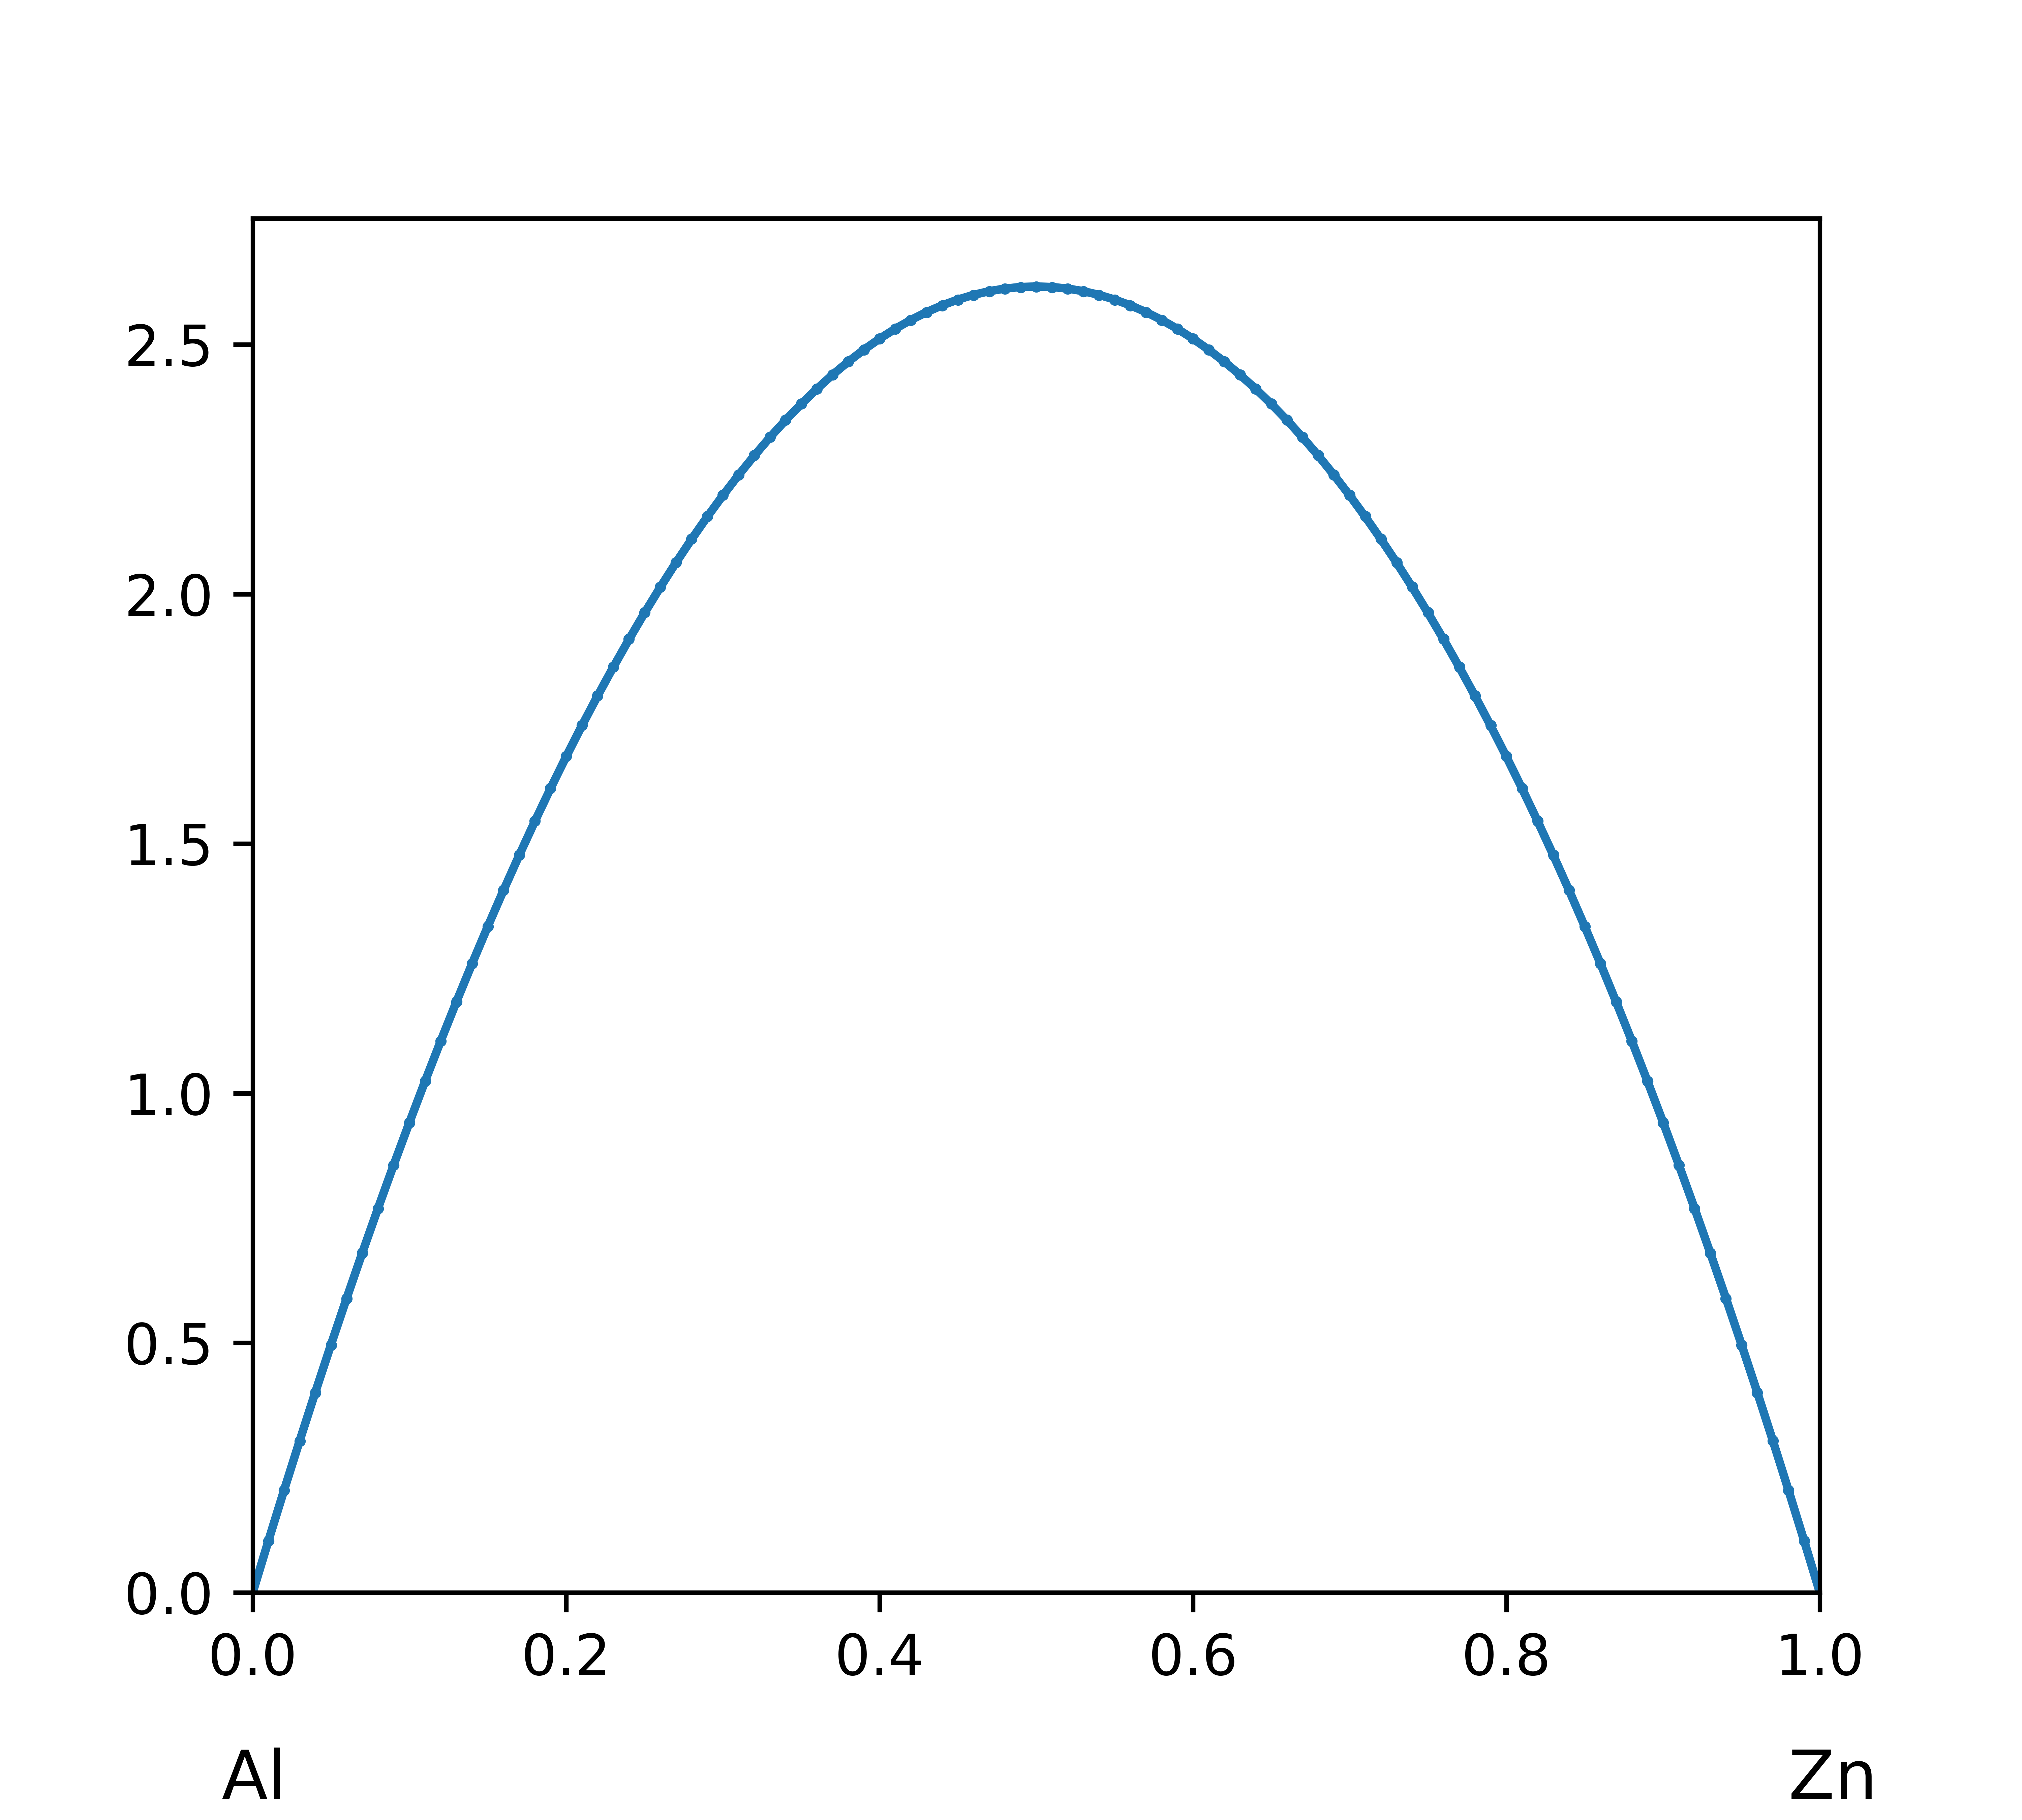
\includegraphics[width=1\linewidth]{Al-Zn_Enthalpy}
  \caption{Enthalpy of Mixing (kJ/mol)}
  \label{fig:sub2}
\end{subfigure}
\caption{System Al-Zn (T = 1073 K): solid lines -- \cite{Al-Zn_Data}; dotted lines - TISR}
\label{fig:Al-Zn}
\end{figure}

\begin{figure}
\centering
\begin{subfigure}{.5\textwidth}
  \centering
  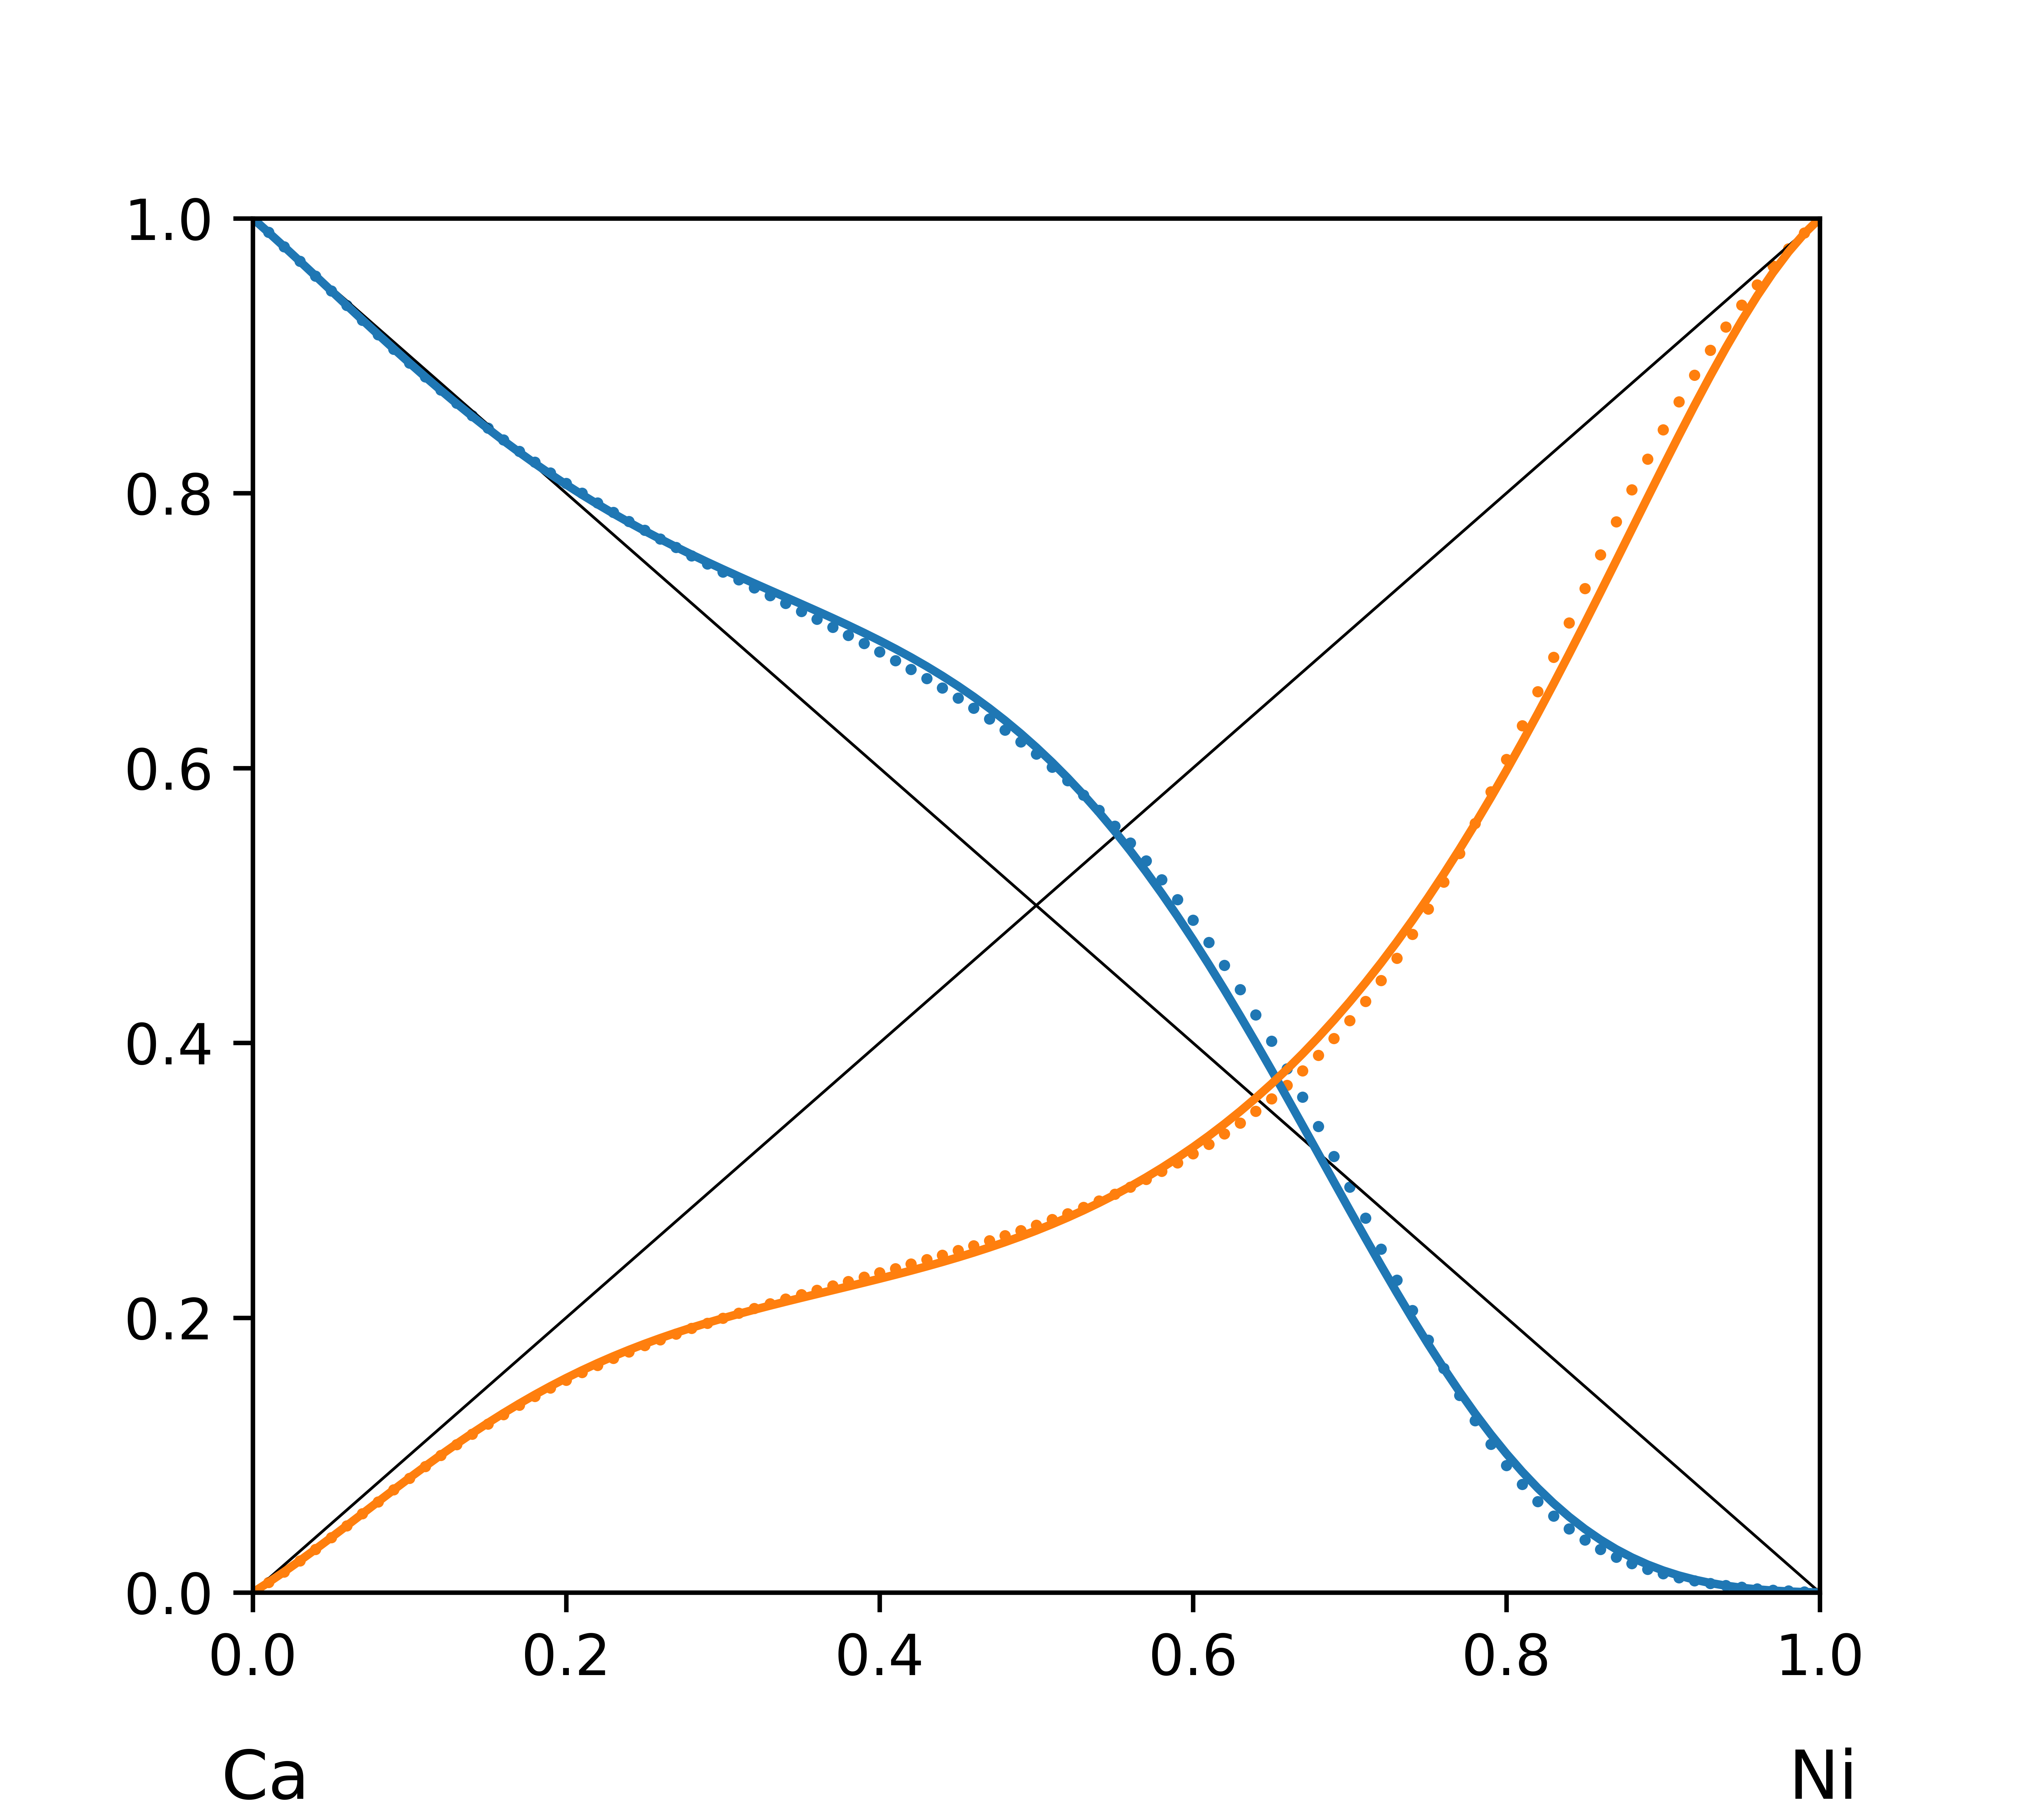
\includegraphics[width=1\linewidth]{Ca-Ni_Activity}
  \caption{Component Activities}
  \label{fig:sub1}
\end{subfigure}%
\begin{subfigure}{.5\textwidth}
  \centering
  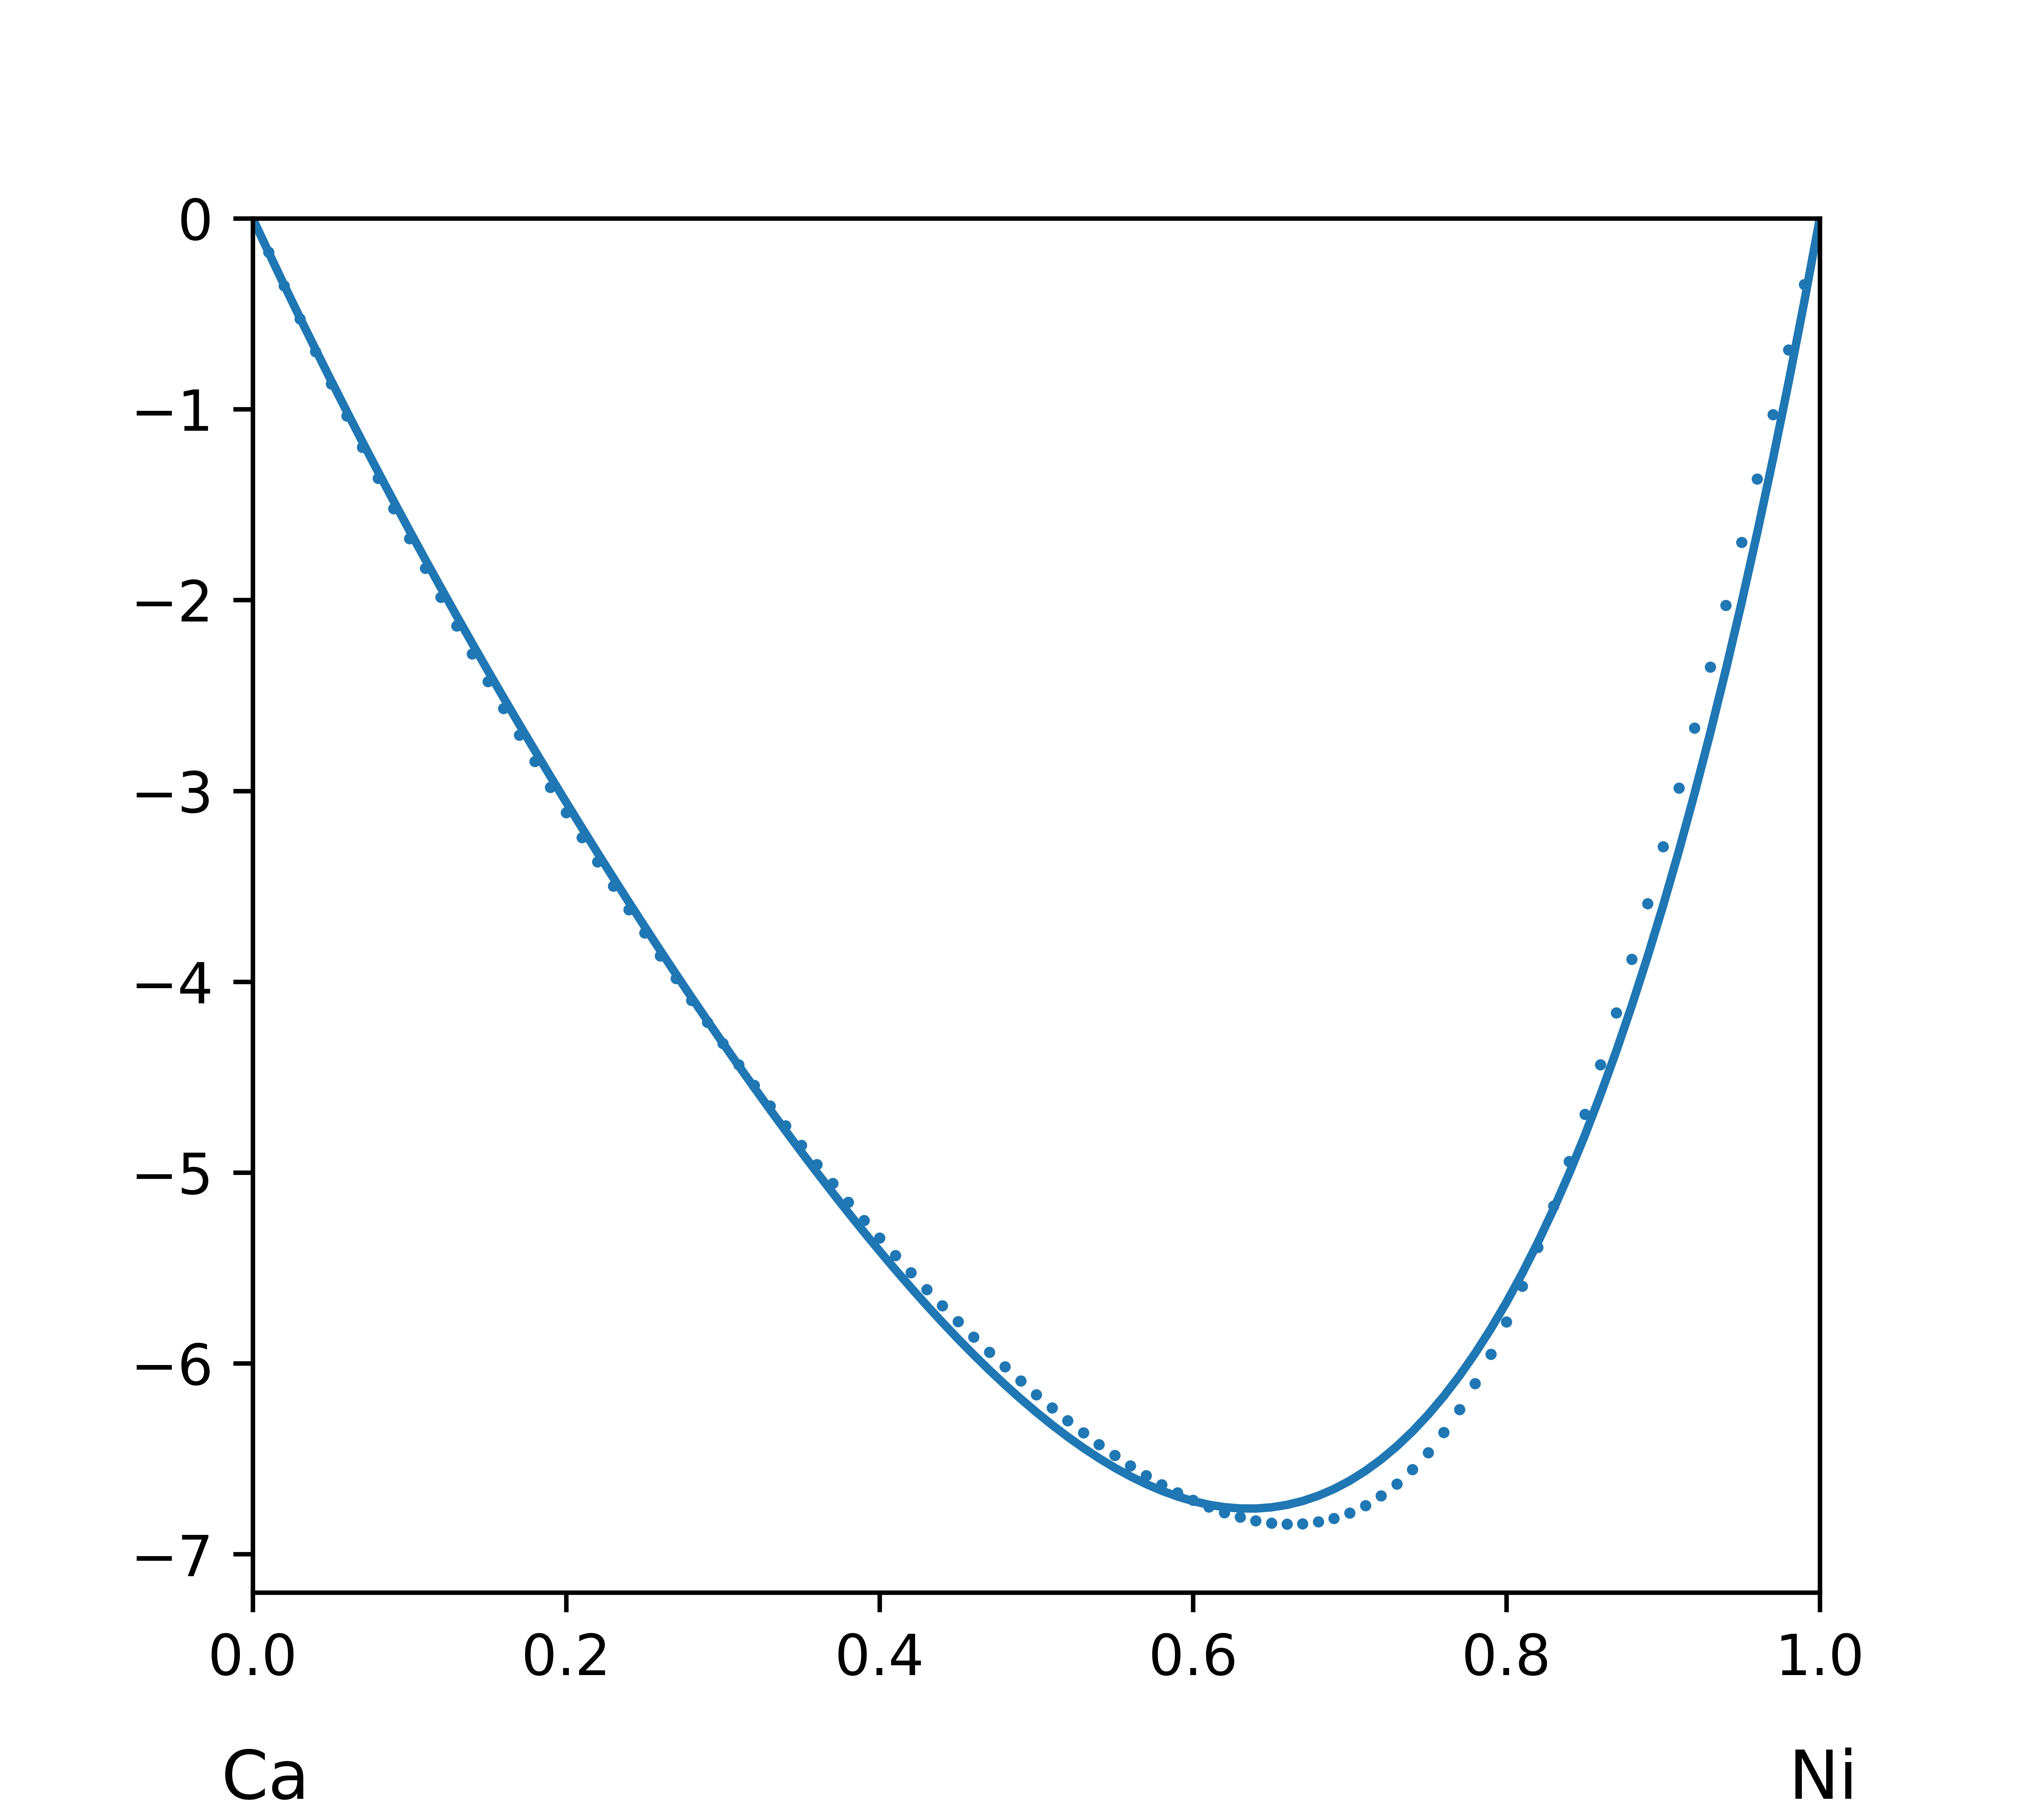
\includegraphics[width=1\linewidth]{Ca-Ni_Enthalpy}
  \caption{Enthalpy of Mixing (kJ/mol)}
  \label{fig:sub2}
\end{subfigure}
\caption{System Ca-Ni (T = 1120 K): solid lines -- \cite{Ca-Ni_Data}; dotted lines - TISR}
\label{fig:Ca-Ni}
\end{figure}


\begin{figure}
\centering
\begin{subfigure}{.5\textwidth}
  \centering
  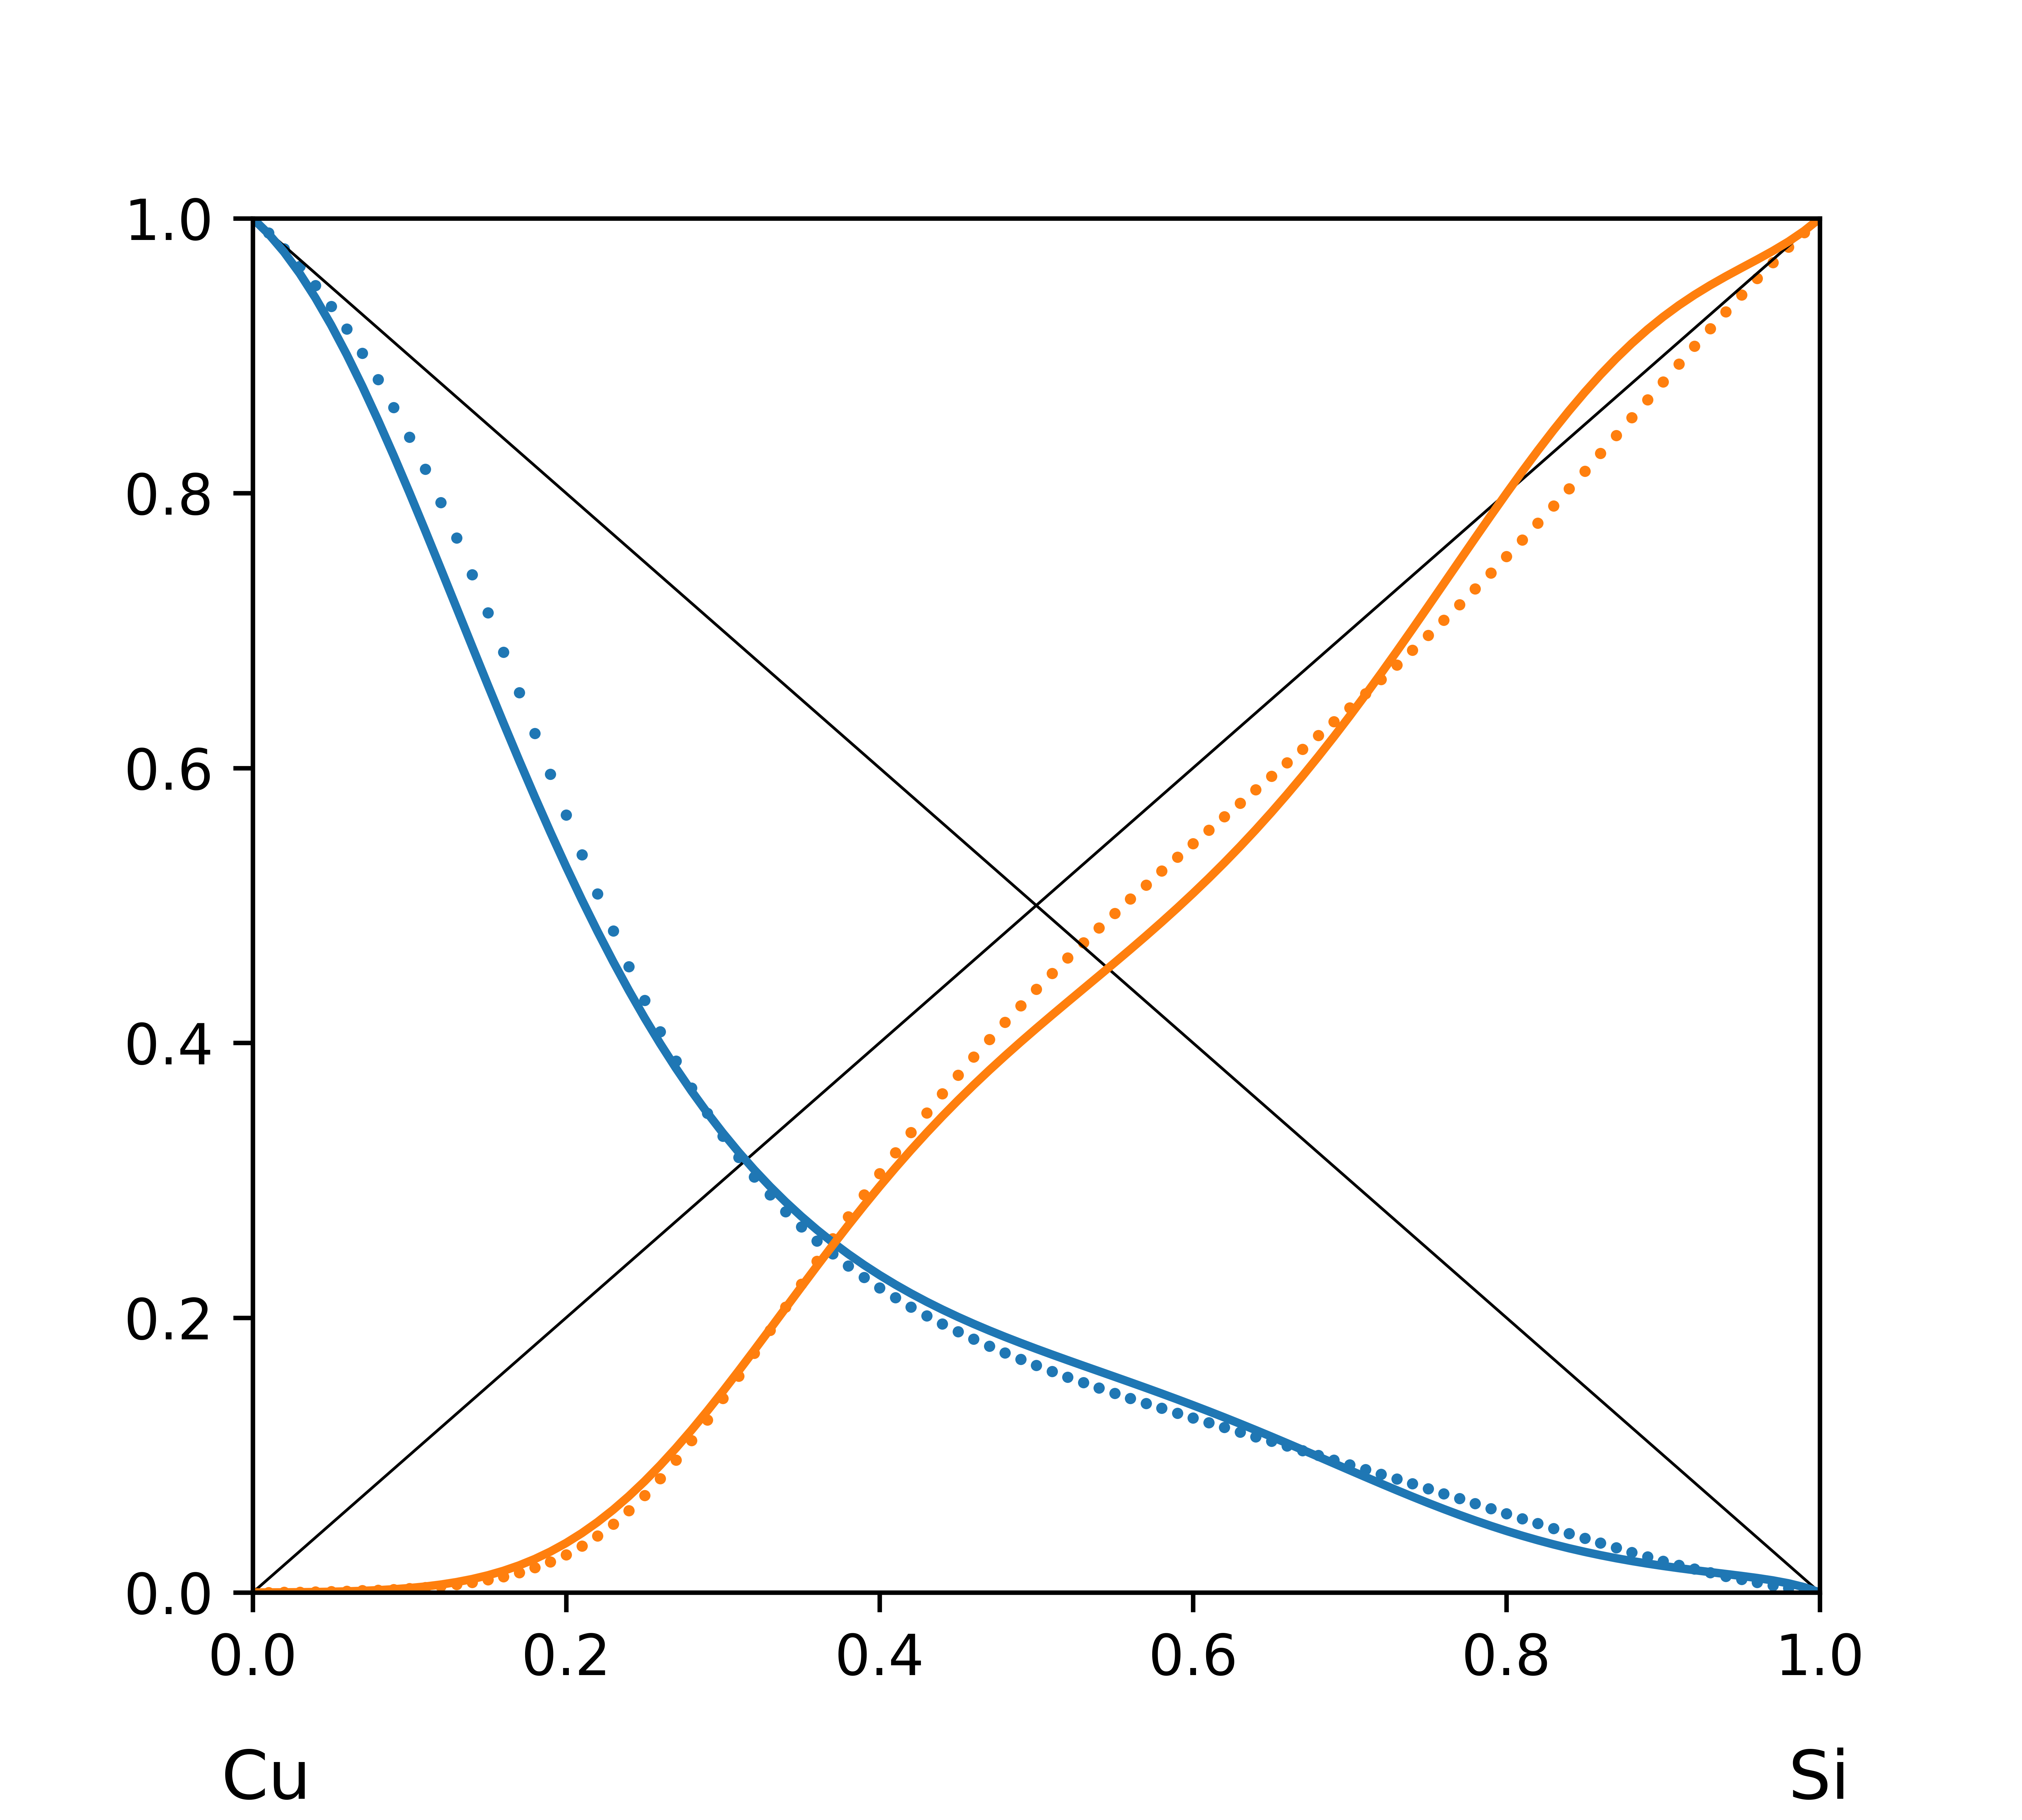
\includegraphics[width=1\linewidth]{Cu-Si2_Activity}
  \caption{Component Activities}
  \label{fig:sub1}
\end{subfigure}%
\begin{subfigure}{.5\textwidth}
  \centering
  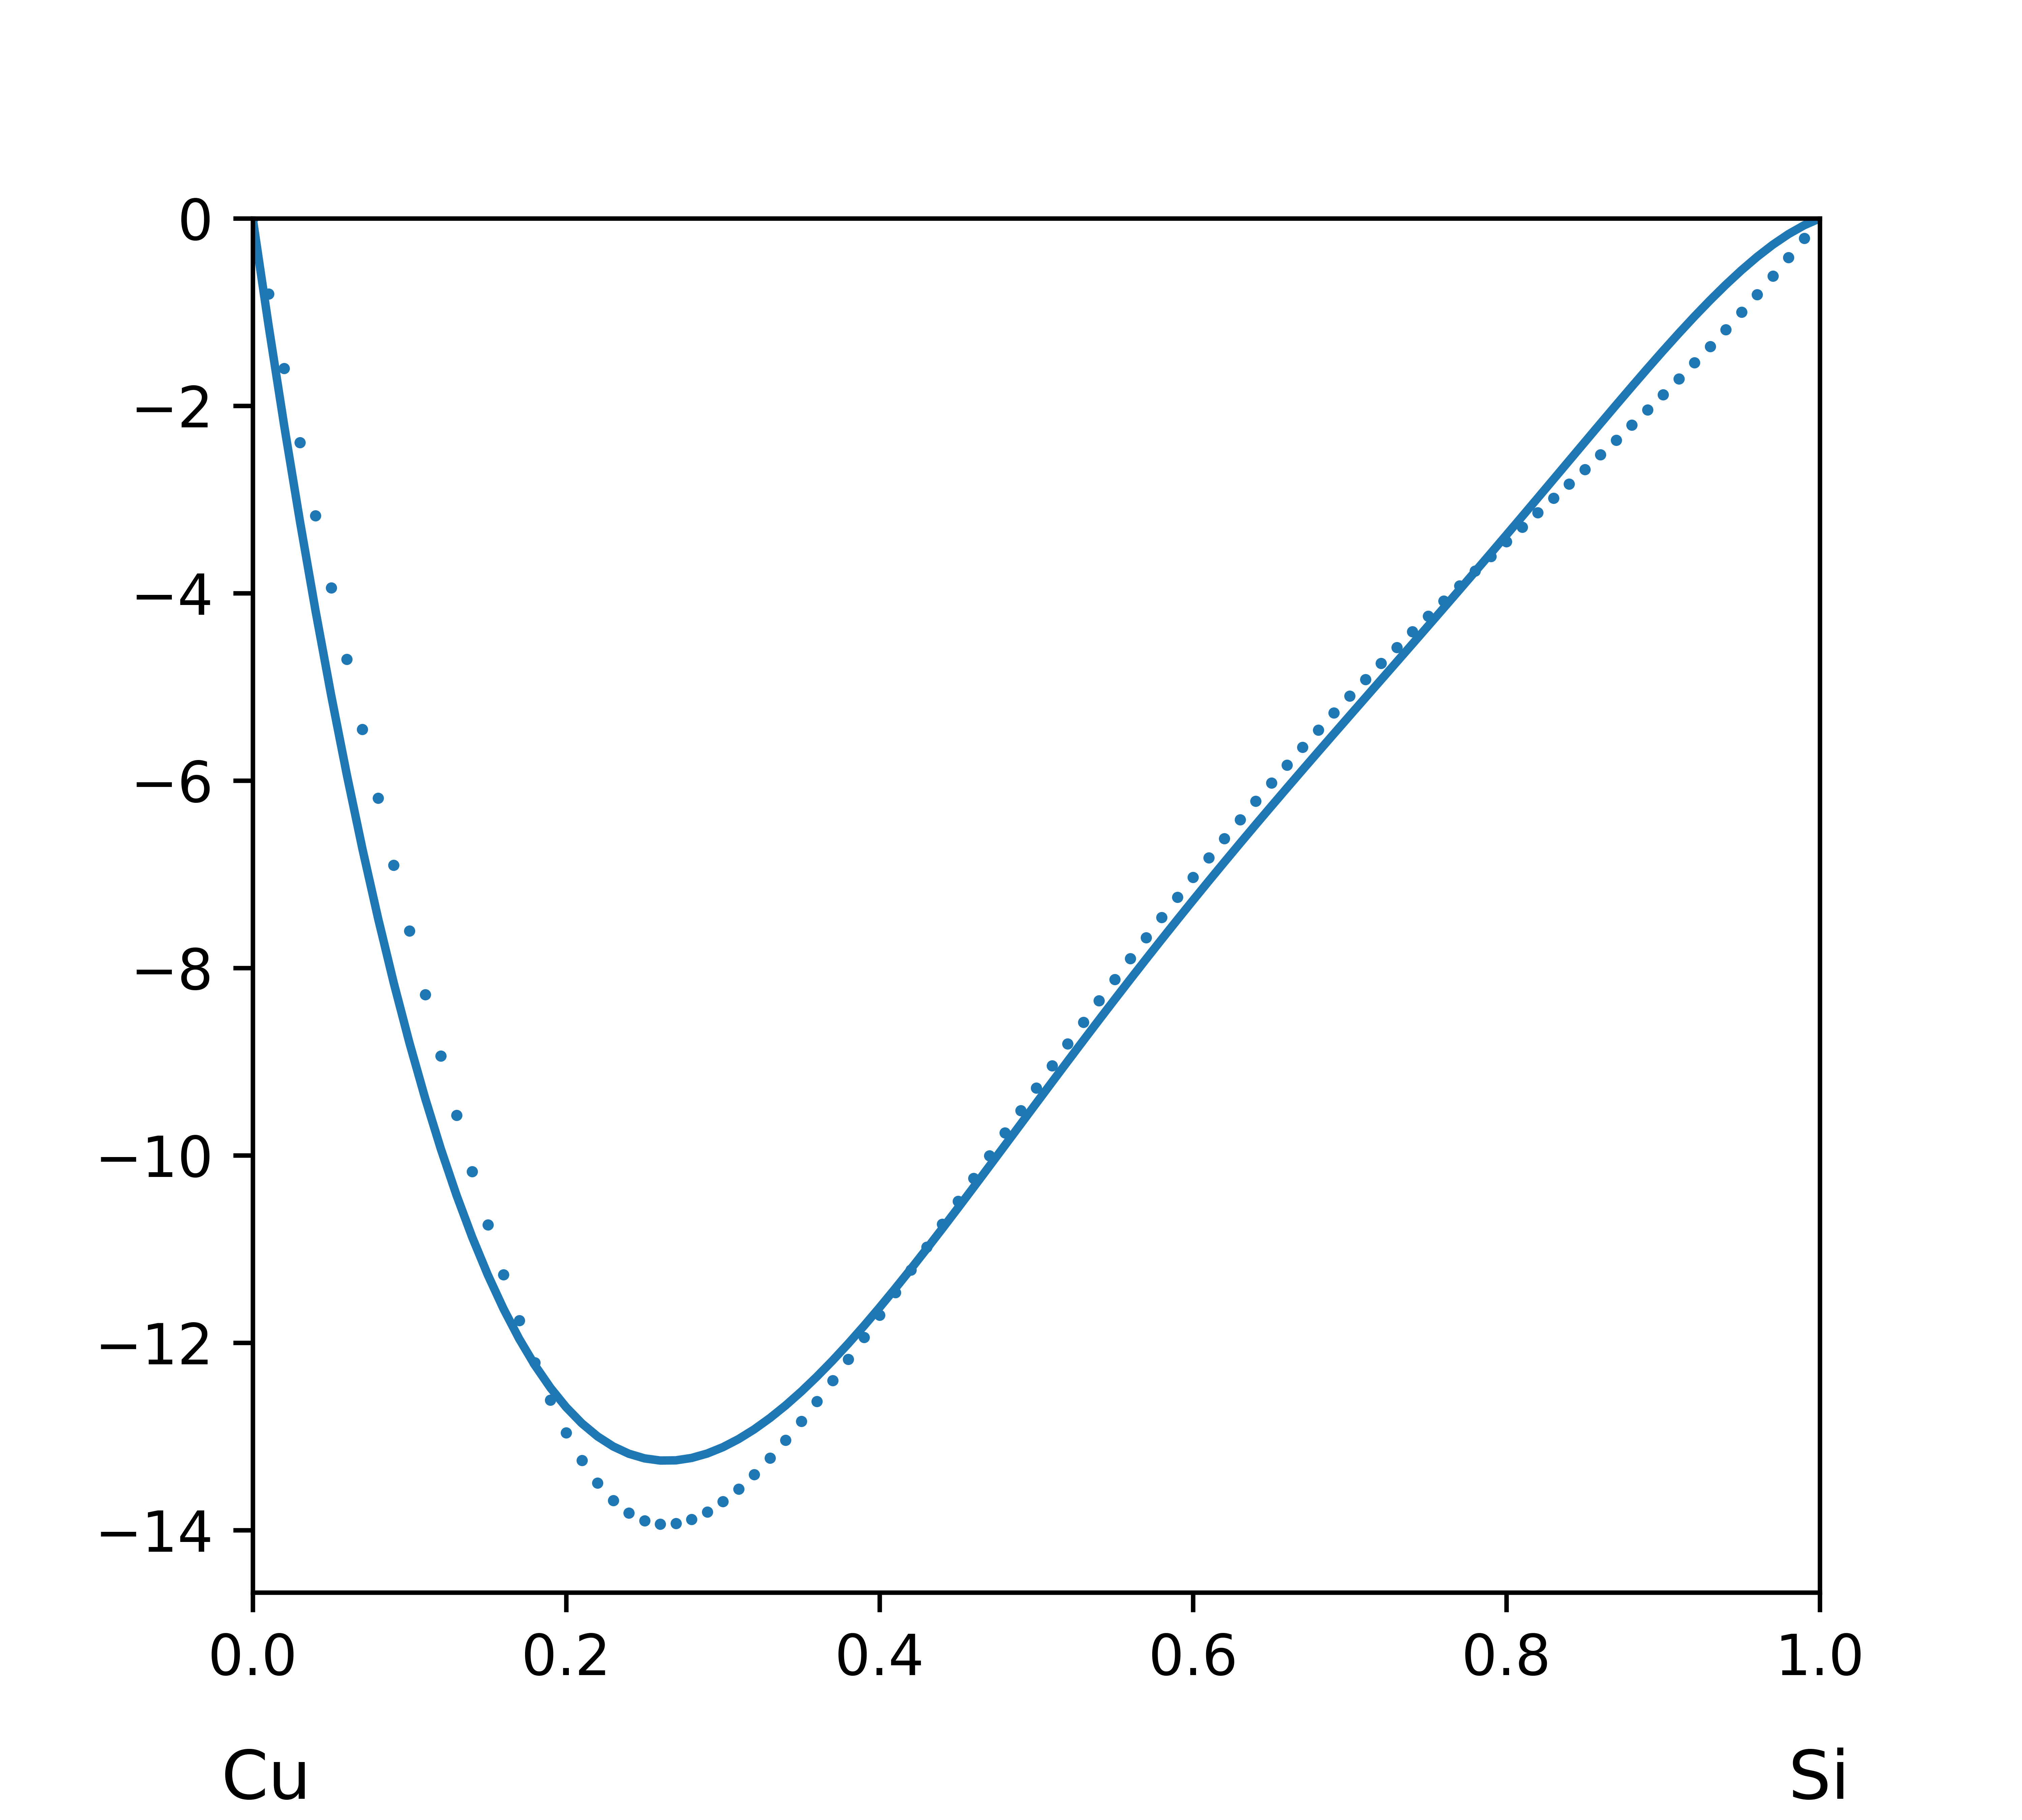
\includegraphics[width=1\linewidth]{Cu-Si2_Enthalpy}
  \caption{Enthalpy of Mixing (kJ/mol)}
  \label{fig:sub2}
\end{subfigure}
\caption{System Cu-Si (T = 1575 K): solid lines -- \cite{Cu-Si2_Data}; dotted lines - TISR} 
\label{fig:Cu-Si2}   
\end{figure}

\begin{figure}
\centering
\begin{subfigure}{.5\textwidth}
  \centering
  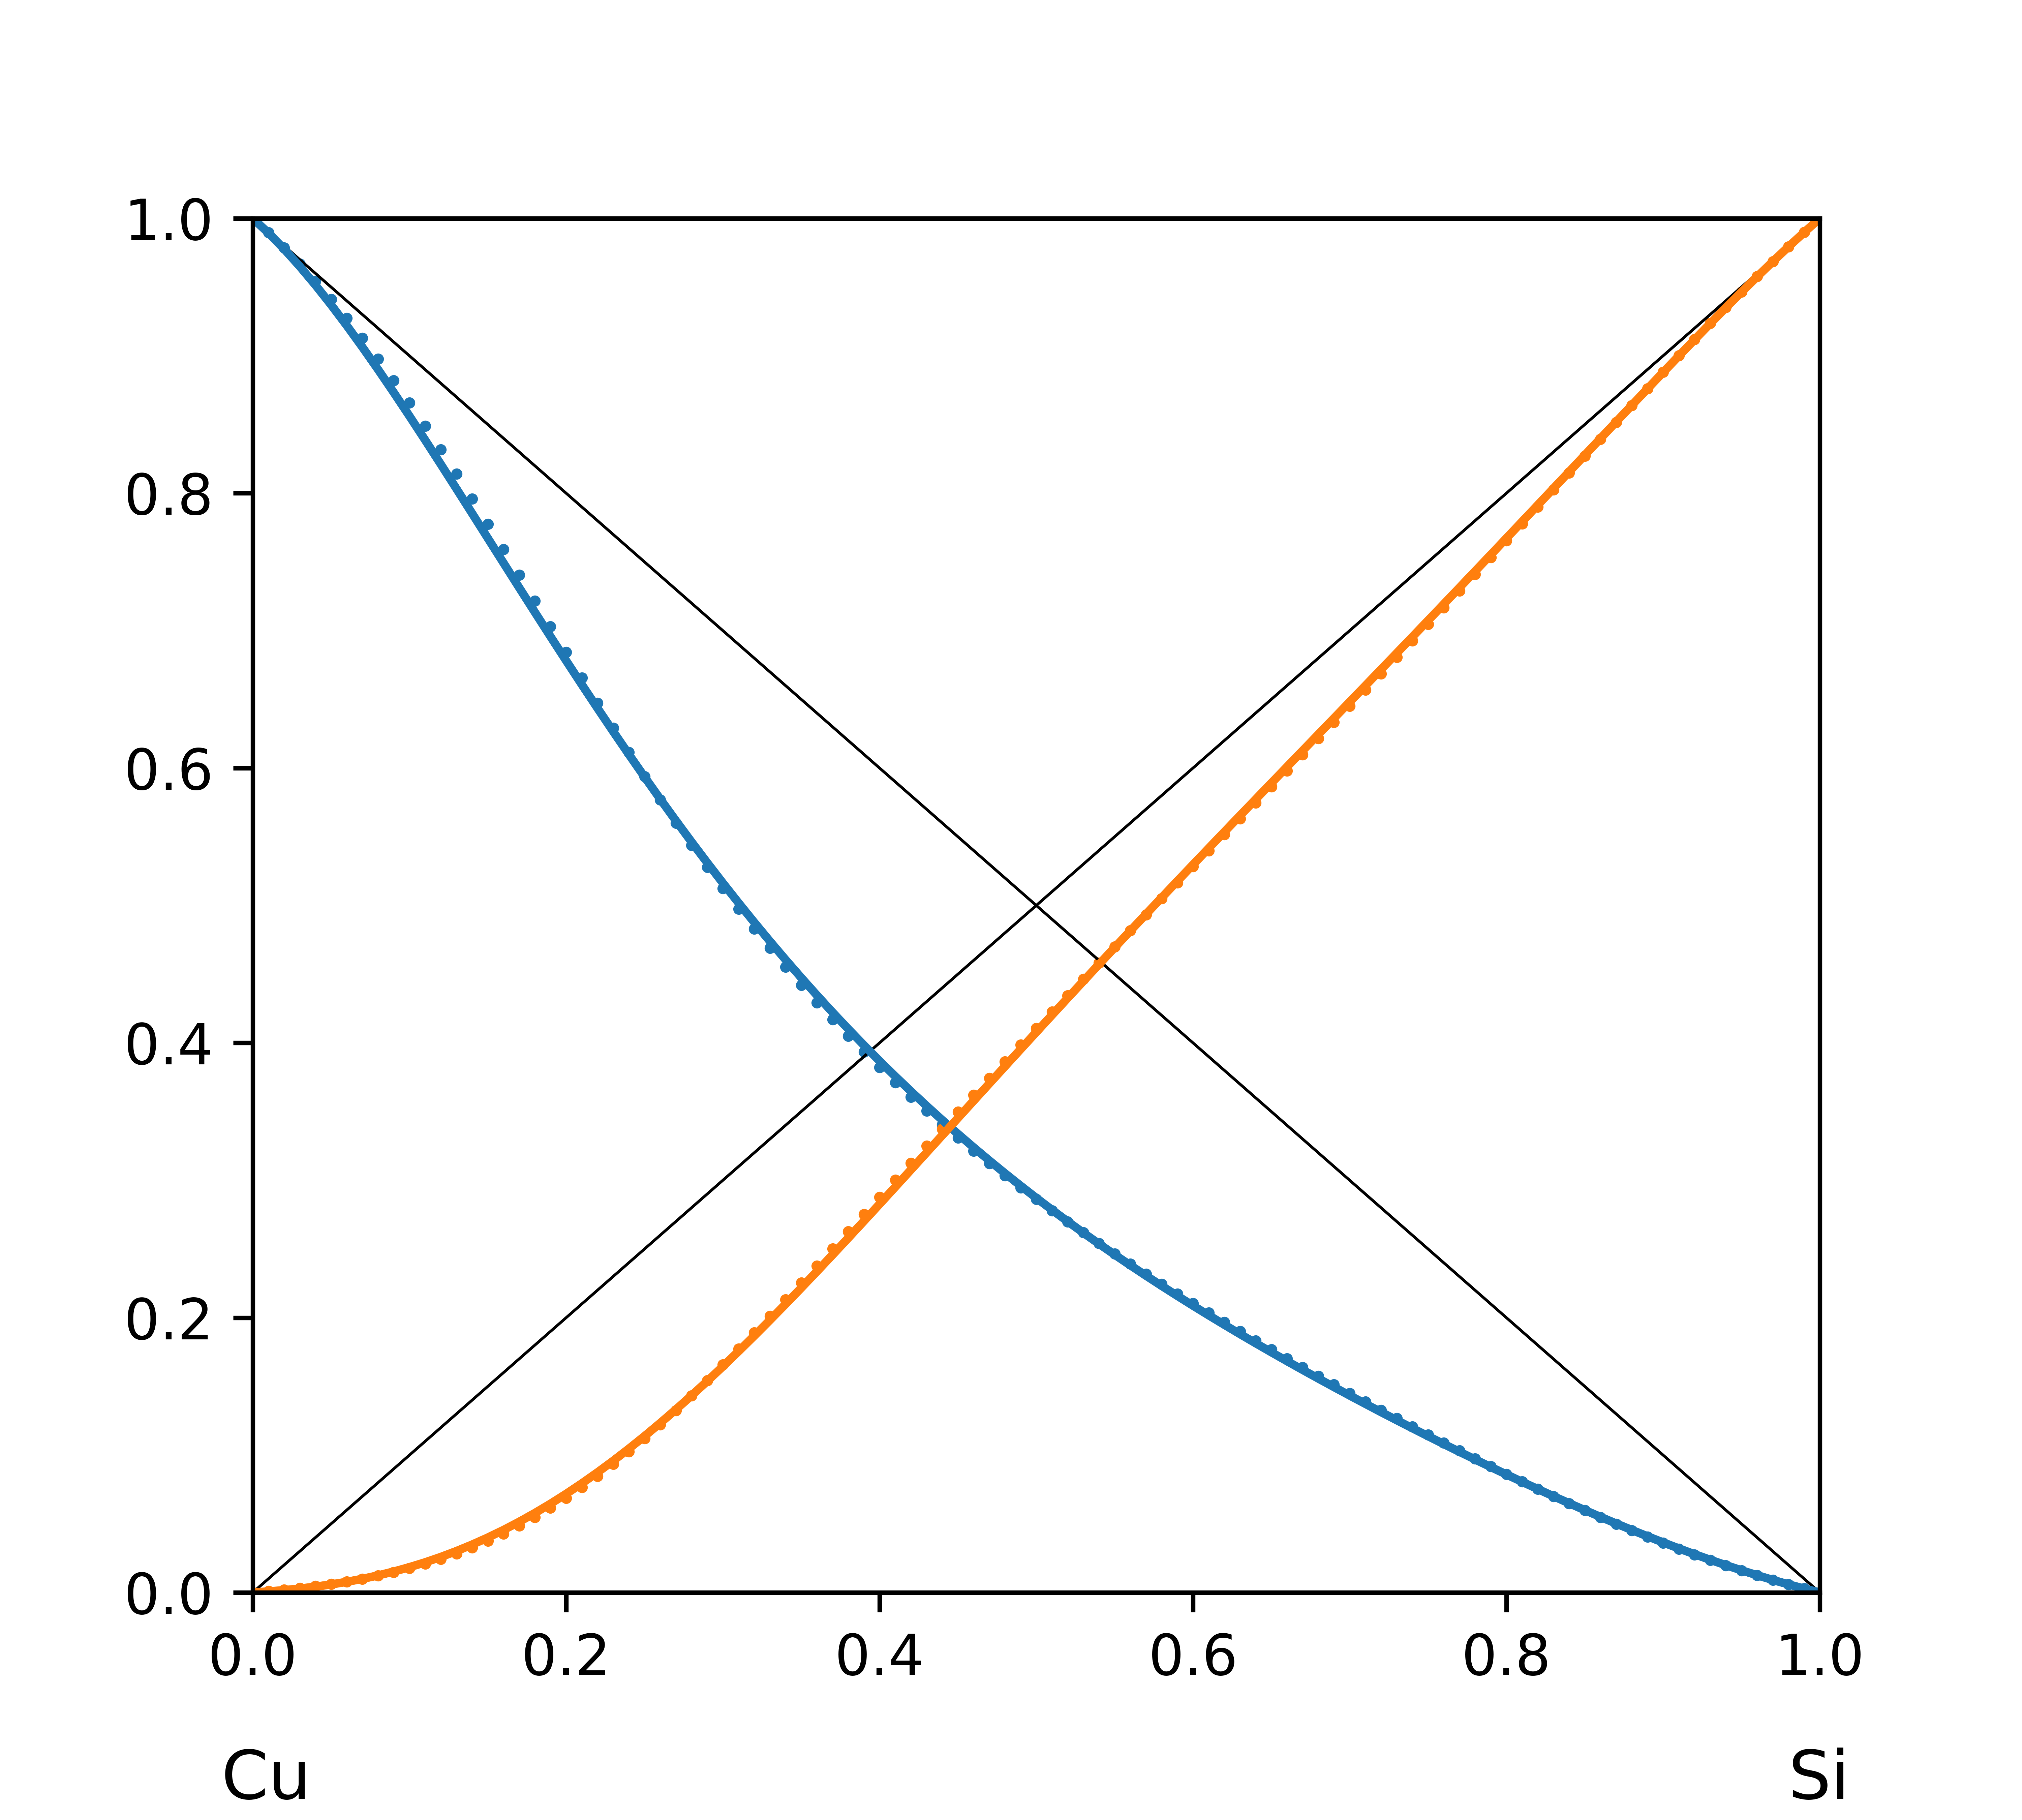
\includegraphics[width=1\linewidth]{Cu-Si_Activity}
  \caption{Component Activities}
  \label{fig:sub1}
\end{subfigure}%
\begin{subfigure}{.5\textwidth}
  \centering
  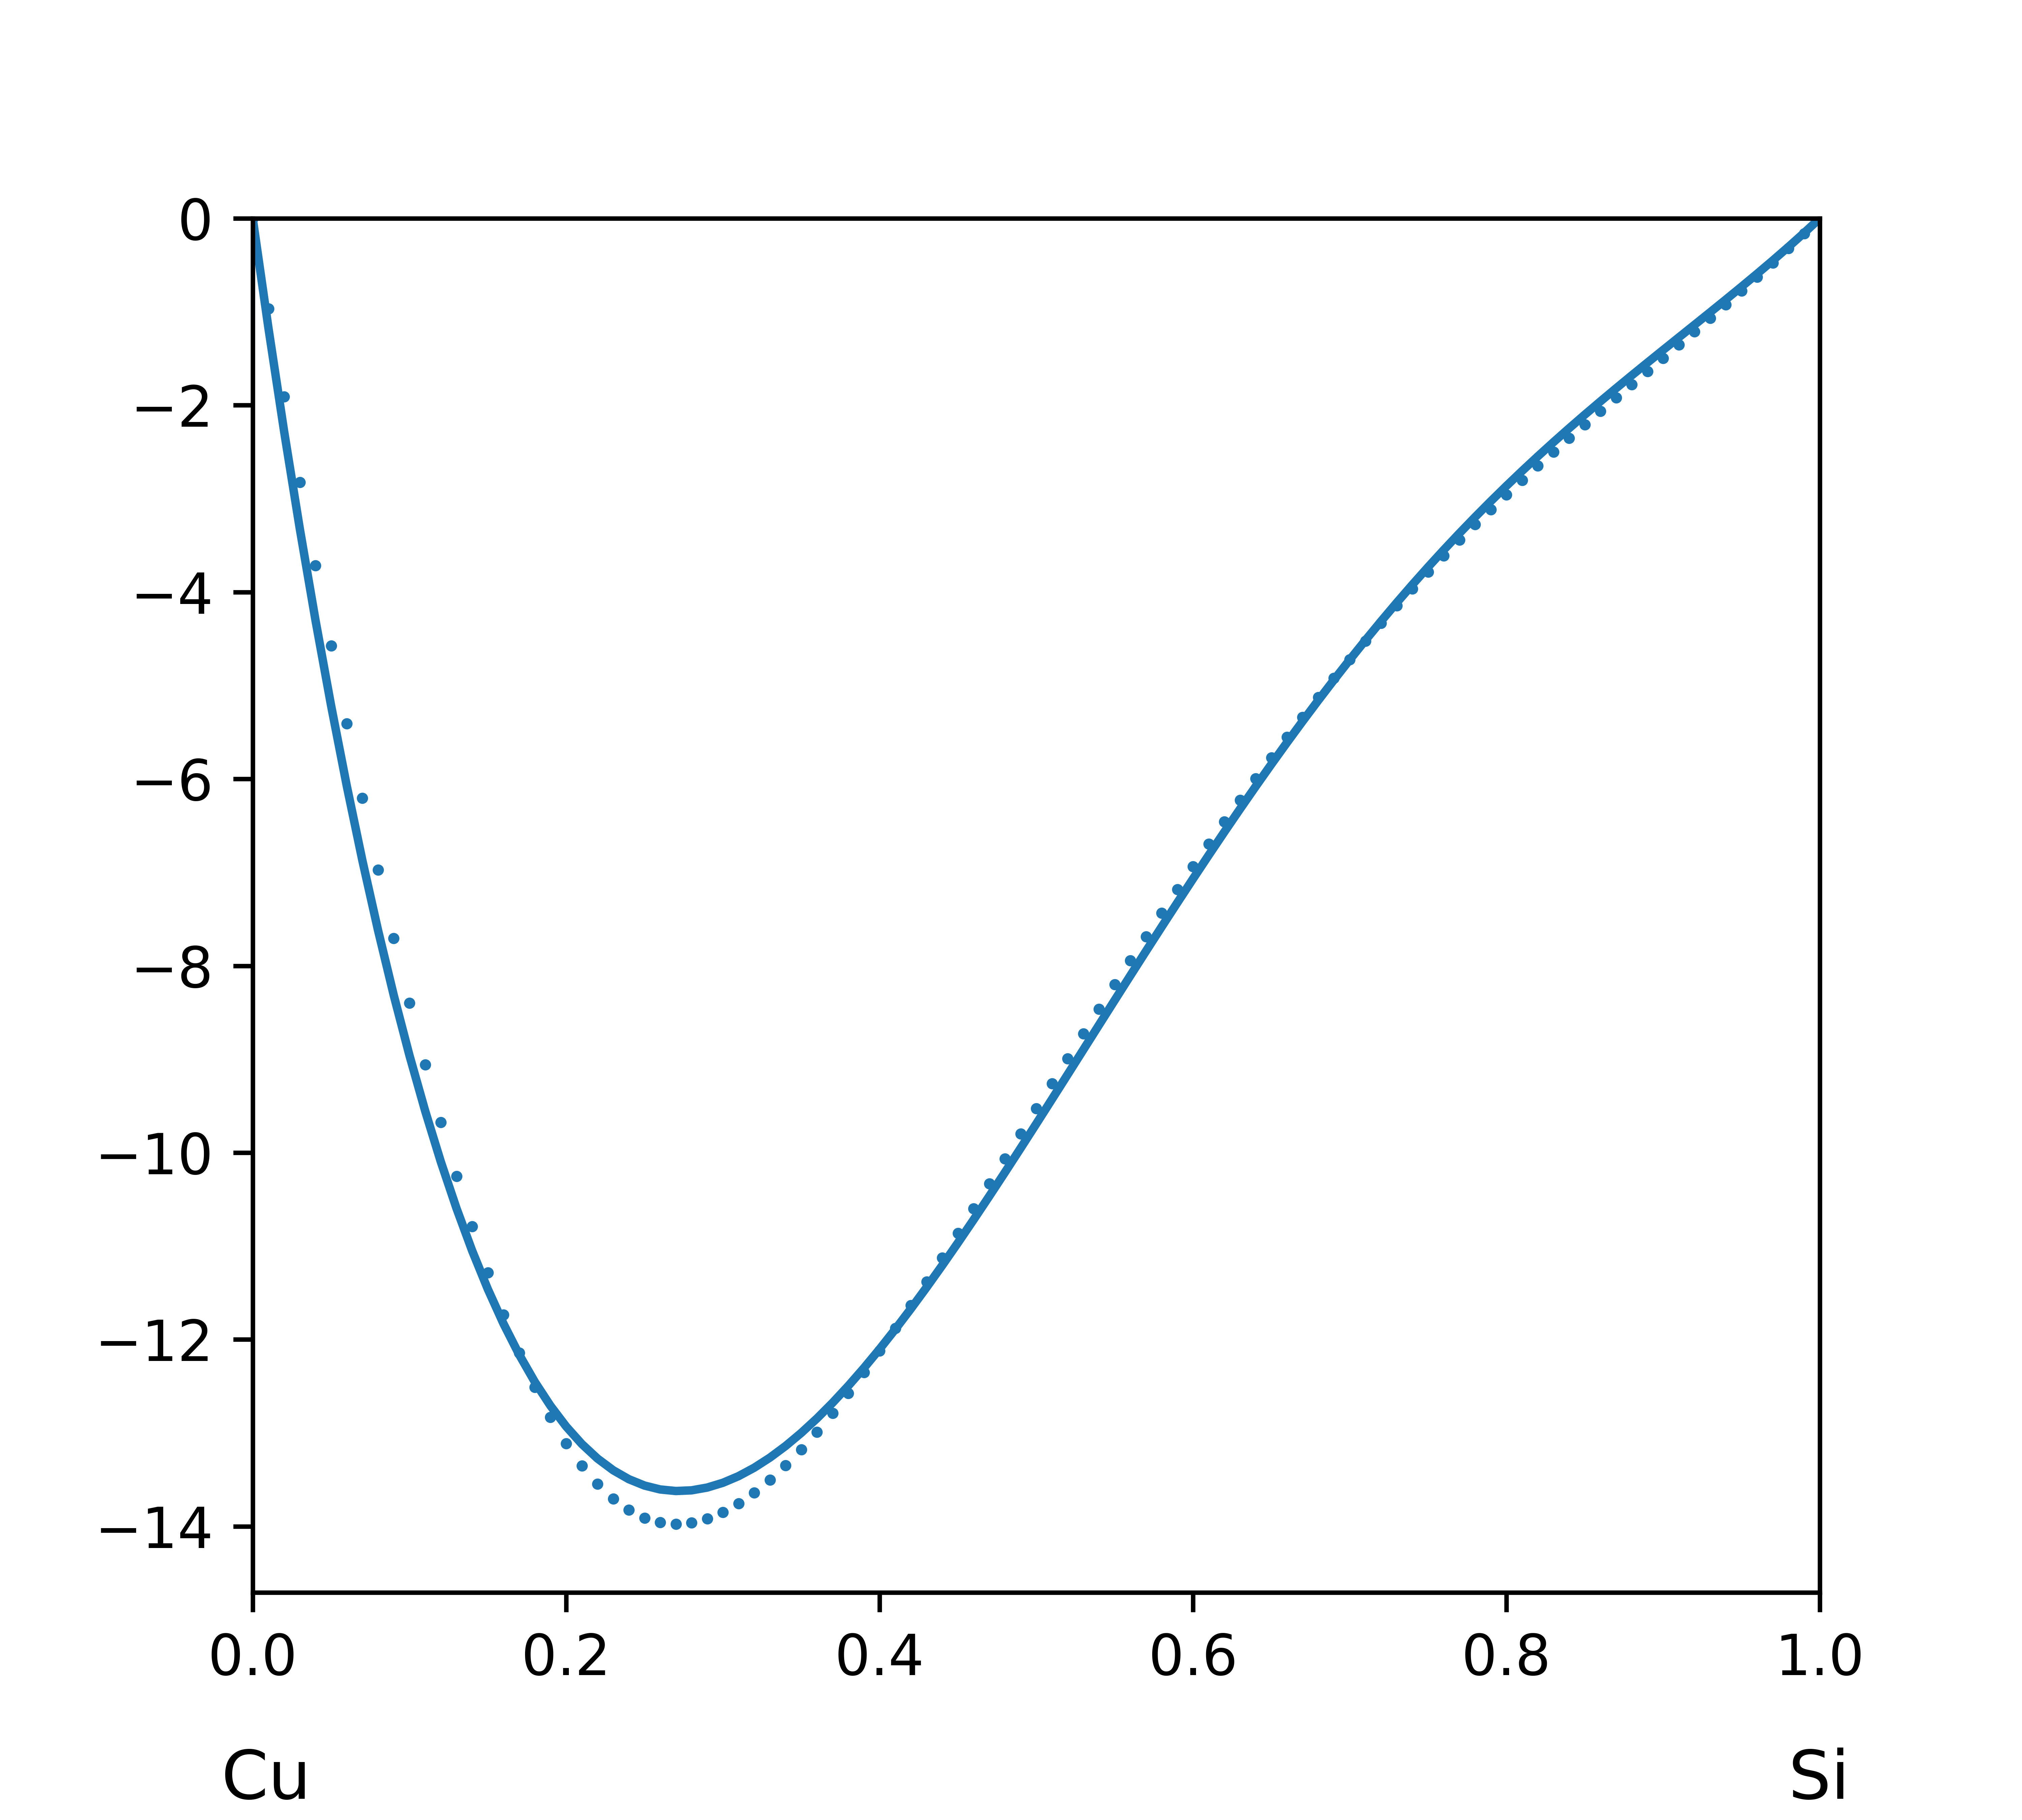
\includegraphics[width=1\linewidth]{Cu-Si_Enthalpy} 
  \caption{Enthalpy of Mixing (kJ/mol)}
  \label{fig:sub2}
\end{subfigure}
\caption{System Cu-Si (T = 1575 K): solid lines -- \cite{Al-Si_Data}; dotted lines - TISR}
\label{fig:Cu-Si} 
\end{figure}


\begin{figure}[h]
\centering
\begin{subfigure}{.5\textwidth}
  \centering
  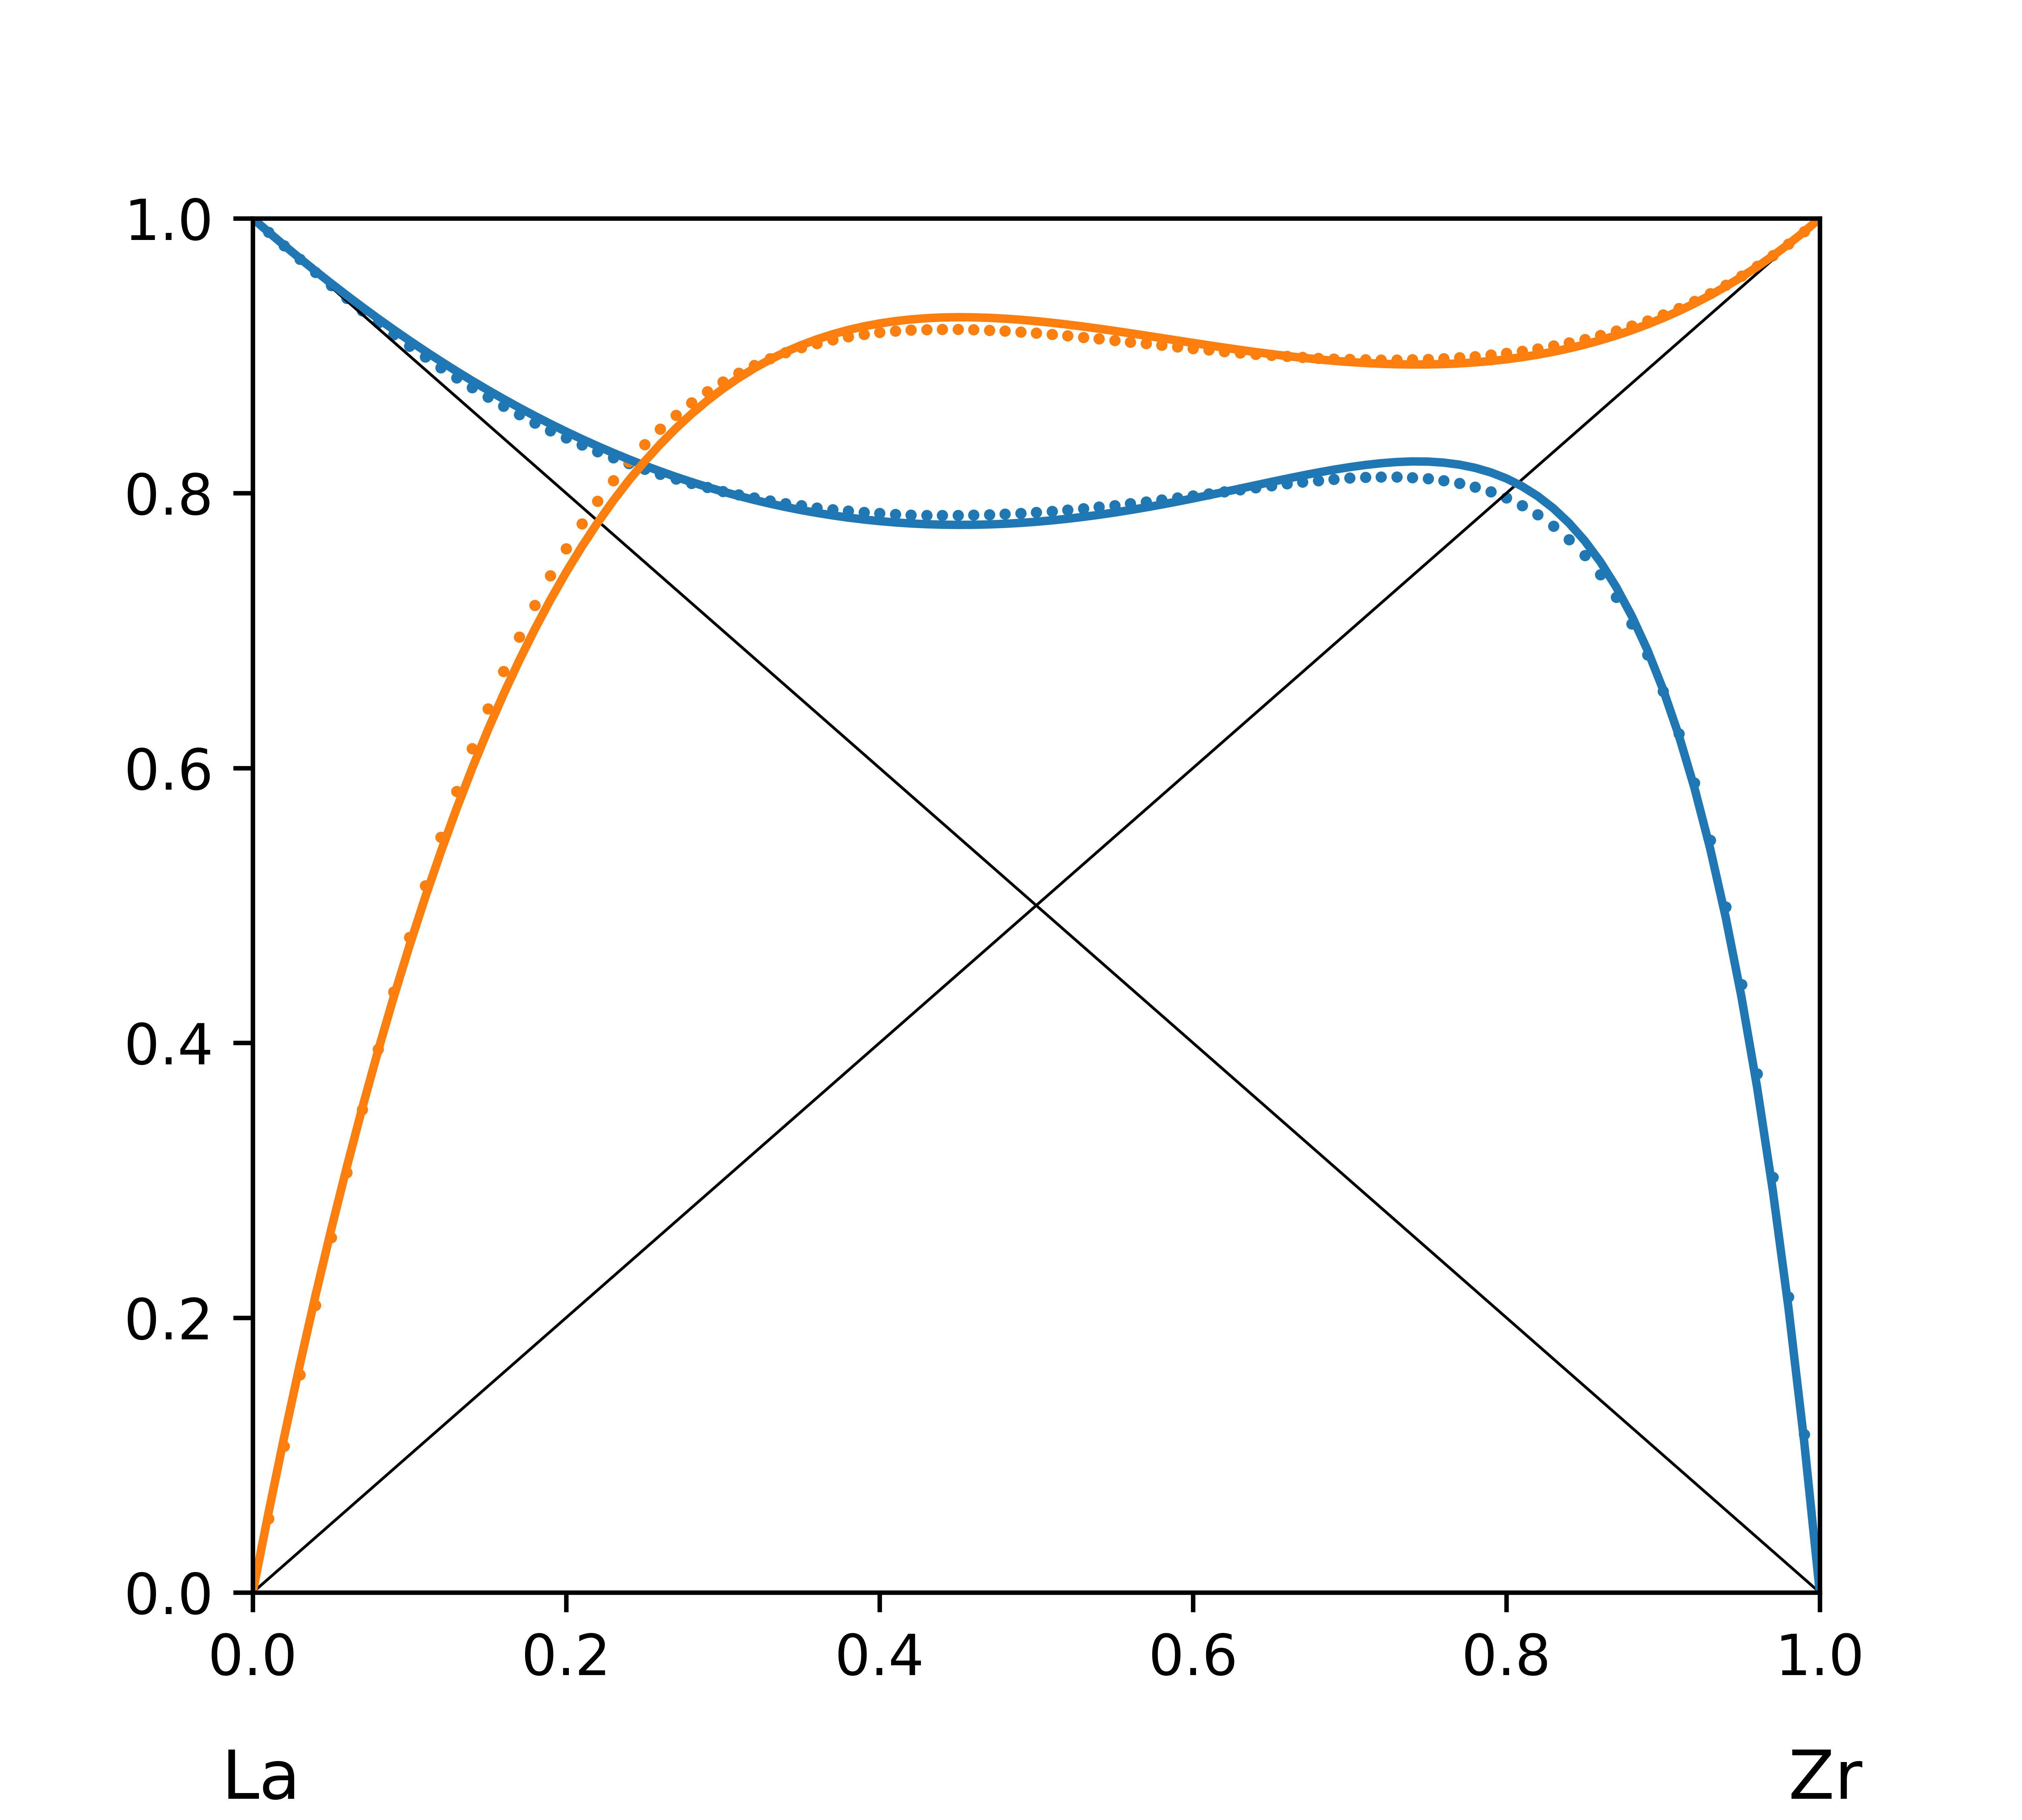
\includegraphics[width=1\linewidth]{La-Zr_Activity}
  \caption{Component Activities}
  \label{fig:sub1}
\end{subfigure}%
\begin{subfigure}{.5\textwidth}
  \centering
  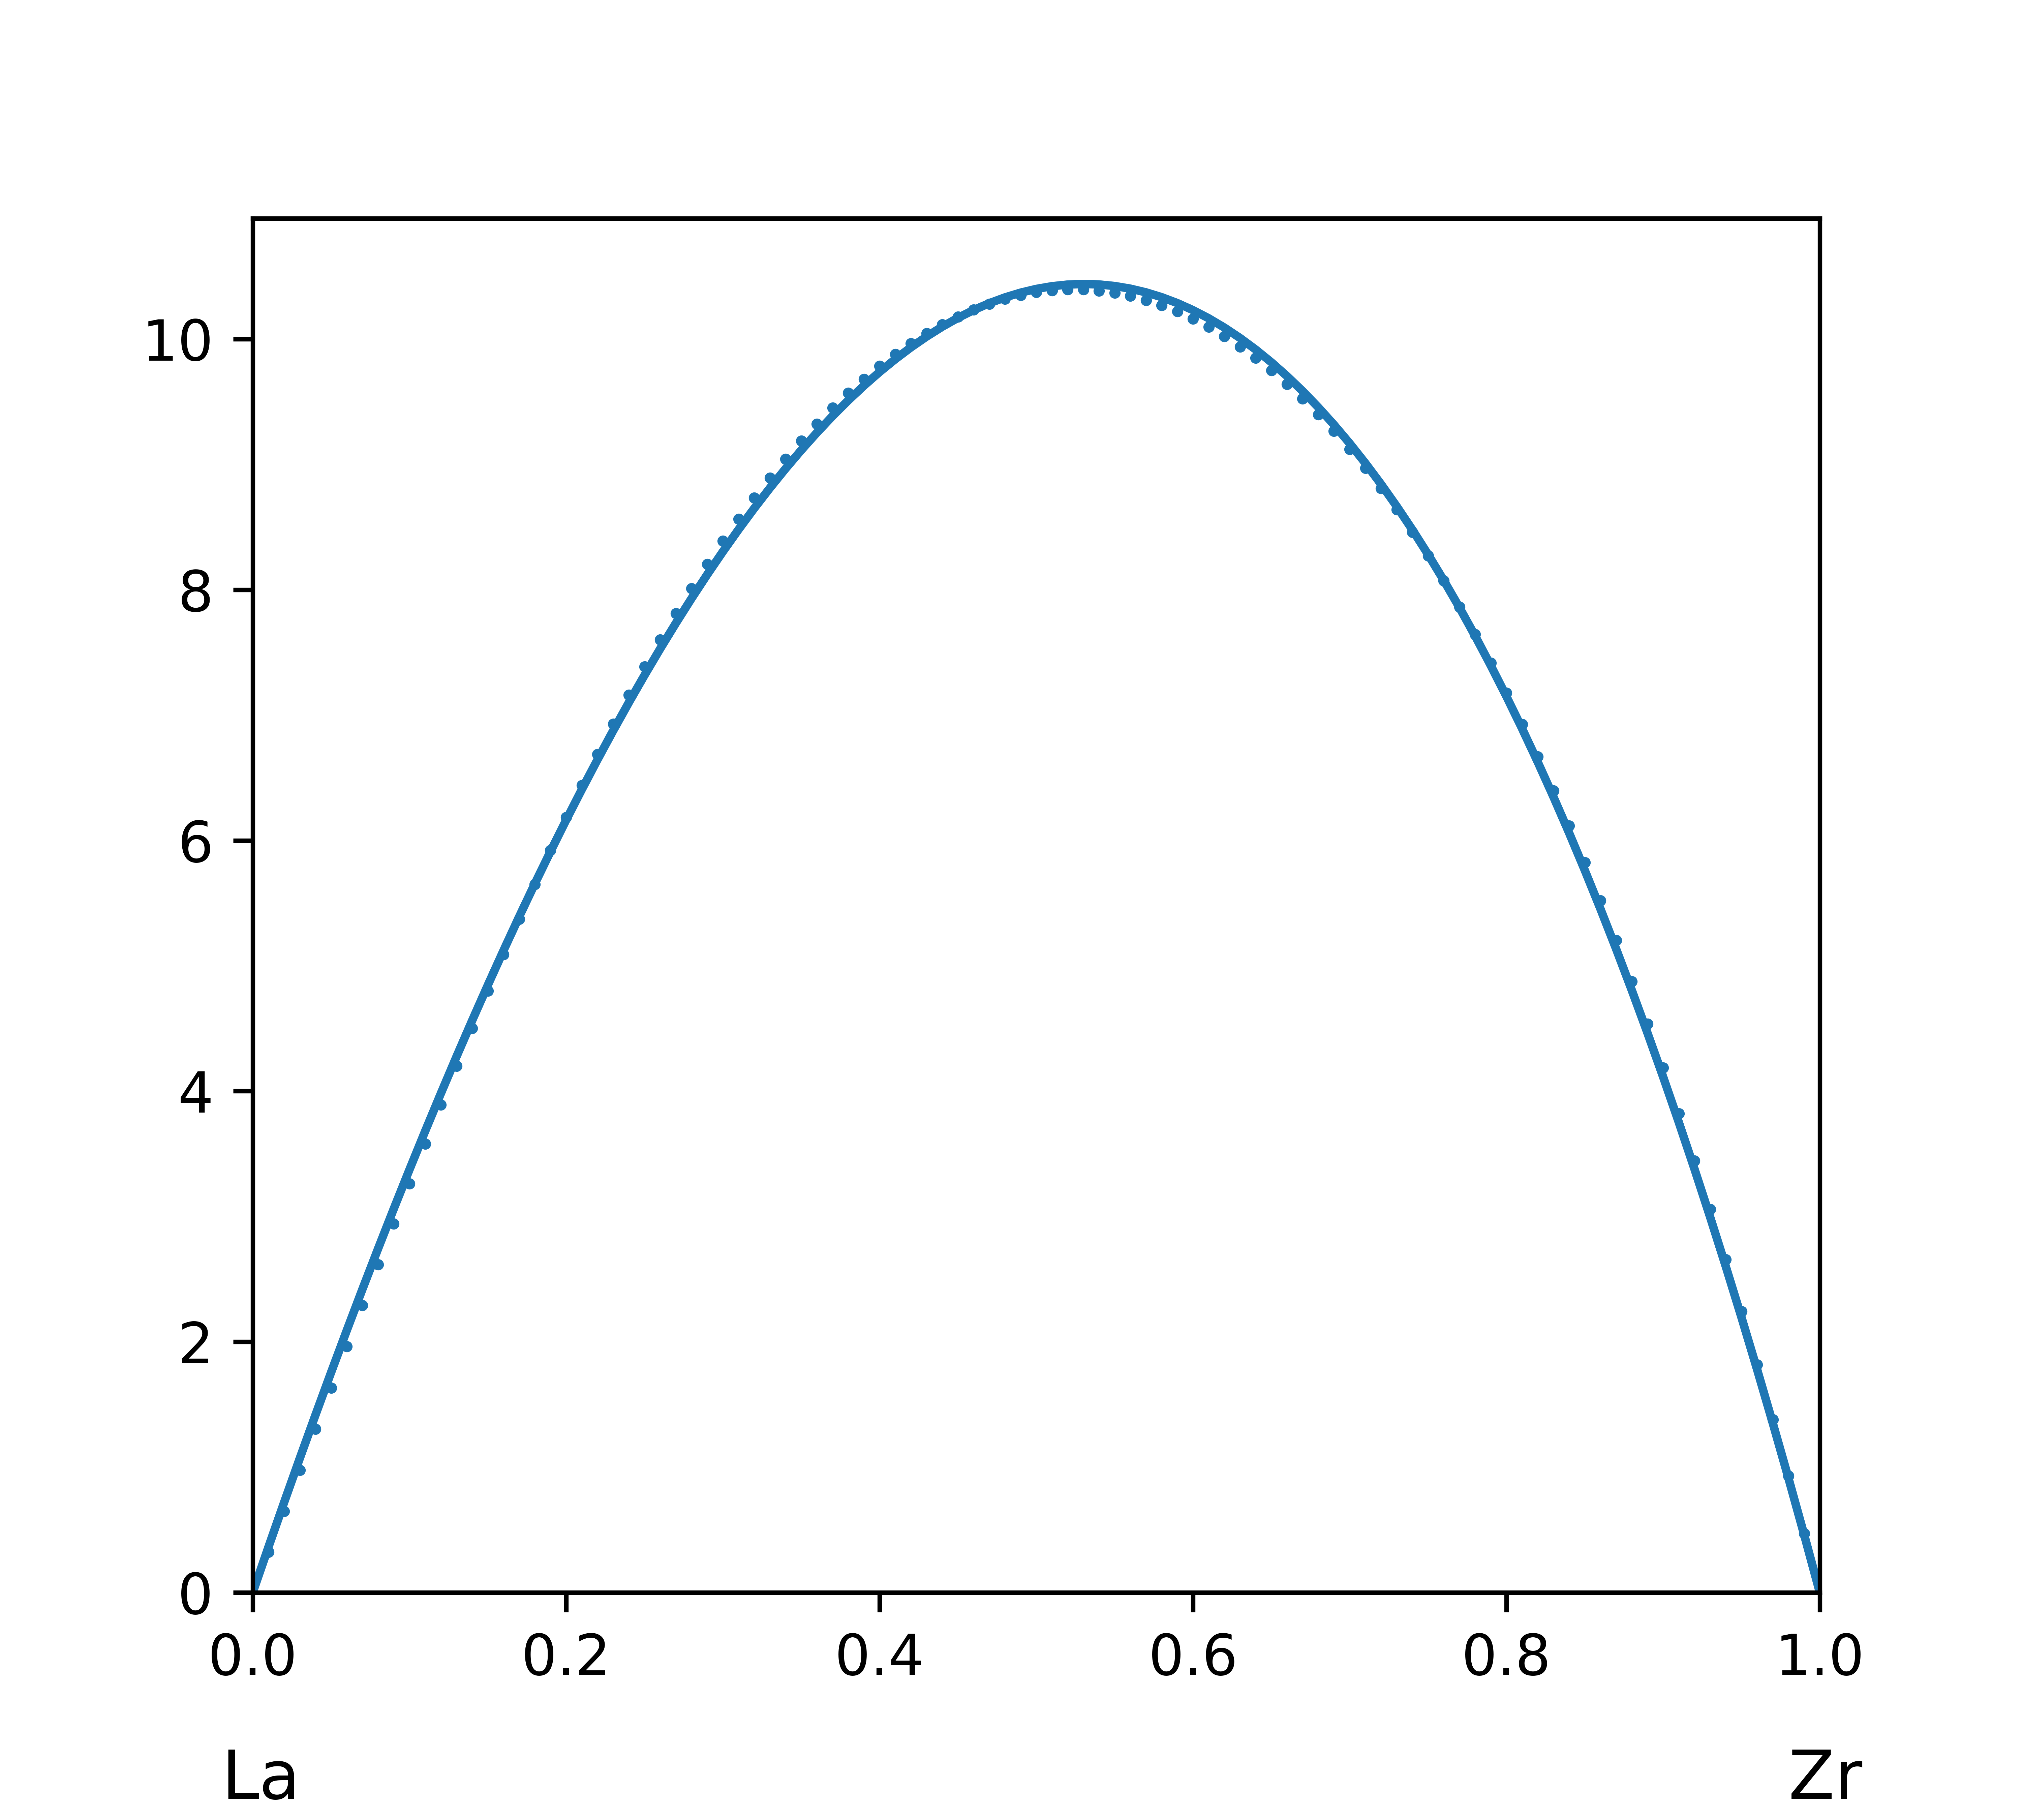
\includegraphics[width=1\linewidth]{La-Zr_Enthalpy}
  \caption{Enthalpy of Mixing (kJ/mol)}
  \label{fig:sub2}
\end{subfigure}
\caption{System La-Zr (T = 1800 K): solid lines -- \cite{La-Zr_Data}; dotted lines - TISR}
\label{fig:La-Zr}
\end{figure}





\end{document}

It is possible also -- as will be shown in the forth part of this article -- to change the definition of $\gamma$ parameter for the systems with positive deviations from ideality in the way that will  ensure reproduction of correct critical temperature of immiscibility and improvement of all other thermodynamic characteristics.

-----------------------------------

The definition of $\gamma$

In fact, the transition from the equation (\ref{config_1}) to the final equation (\ref{config_final}) (that is the actual definition of $\gamma$) is based on arbitrary assumption that  two cell ensembles  are completely autonomous and influence the combinatorial factor independently.

In fact, the transition from the equation (\ ref {config_1}) to the final equation (\ ref {config_final}), which defines $ \ gamma $, is based on the arbitrary assumption that the two ensembles of cells are fully autonomous and independently influence the combinatorial factor.